\documentclass[10pt,journal]{./IEEE_latex_class/IEEEtran}

% In order to reference go to http://truben.no/latex/bibtex/

% *** CITATION PACKAGES ***
\usepackage{cite}

% *** GRAPHICS RELATED PACKAGES ***
%
\ifCLASSINFOpdf
   \usepackage[pdftex]{graphicx}
  % declare the path(s) where your graphic files are
  \graphicspath{{./Figures/}}
  % and their extensions so you won't have to specify these with
  % every instance of \includegraphics
  \DeclareGraphicsExtensions{.pdf,.jpeg,.png}
\else
  % or other class option (dvipsone, dvipdf, if not using dvips). graphicx
  % will default to the driver specified in the system graphics.cfg if no
  % driver is specified.
  % \usepackage[dvips]{graphicx} 
  % declare the path(s) where your graphic files are 
  % \graphicspath{{../eps/}}   
  % and their extensions so you won't have to specify these with
  % every instance of \includegraphics
  % \DeclareGraphicsExtensions{.eps}
\fi


% *** MATH PACKAGES ***
\usepackage[cmex10]{amsmath}
\usepackage{amssymb}

% correct bad hyphenation here
\hyphenation{op-tical net-works semi-conduc-tor}

%  OTHER PACKAGES

\usepackage{float,amsfonts,multicol,fancyvrb,lastpage,ragged2e,url,color,lipsum,enumerate,todonotes,chemfig,fixltx2e, epstopdf, subcaption,centernot}
\usepackage[font=footnotesize,labelfont = sf, textfont=sf,labelfont=bf]{caption,subcaption}


\newcounter{MYtempeqncnt}





\begin{document}

%
% paper title
% can use linebreaks \\ within to get better formatting as desired
\title{Computational design of RNA-based oscillatory circuits}

\author{J.~Binysh
        \\ \IEEEmembership{* University of Warwick, Complexity Department}}

% The paper headers
\markboth{hi}%
{Parameter estimation of RNA-based oscillatory circuits}

% make the title area
\maketitle

% This defines the title + page out of # of pages at the heading of the pages
\thispagestyle{empty}

\newcommand{\MYheader}{\smash{\scriptsize

\hfil\parbox[t][\height][t]{\textwidth}{\centering {\normalsize
Place conference title here}}\hfil\hbox{}}}
\makeatletter

\if@twoside
  \def\ps@headings{%
      \let\@oddfoot\@empty\let\@evenfoot\@empty
      \def\@evenhead{\small\thepage\hfil\leftmark\strut\vadjust{\vskip .1ex\hrule}}%
      \def\@oddhead{\small\rightmark\hfil\thepage\strut\vadjust{\vskip .1ex\hrule}}%
      \let\@mkboth\markboth
    \def\chaptermark##1{%
      \markboth{\scshape%
        \ifnum \c@secnumdepth >\m@ne
            \@chapapp\ \thechapter. \ %
        \fi
        ##1}{}}%
    \def\sectionmark##1{%
      \markright{\scshape%
        \ifnum \c@secnumdepth >\z@
          \thesection. \ %
        \fi
        ##1}}}
\else
  \def\ps@headings{%
    \let\@oddfoot\@empty
    \def\@oddhead{{\slshape\rightmark}\hfil\thepage\ of\ \pageref{LastPage} \strut\vadjust{\vskip .1ex\hrule}}%
    \let\@mkboth\markboth
    \def\chaptermark##1{%
      \markright{\scshape%
        \ifnum \c@secnumdepth >\m@ne
            \@chapapp\ \thechapter. \ %
        \fi
        ##1}}}
\fi
\makeatother

\makeatother

% make changes take effect
\pagestyle{headings}
% adjust as needed
%\addtolength{\footskip}{0\baselineskip}
%\addtolength{\textheight}{-0.1\baselineskip}

\begin{abstract}
For the synthetic biologist looking to engineer regulation of genetic circuitry, RNA is an attractive tool, due to the ease of predicting its behaviour from physiochemical models. In this report, we introduce a system of ODE's to model a recently designed synthetic regulatory circuit, before attempting to estimate its unknown parameters using recent time series data. We provide estimates for a subset of parameters, but find many of them to be inestimable. We discuss why this is this case for our system, and suggest how this problem might be resolved.
\end{abstract}

\IEEEpeerreviewmaketitle


%%%
%%%
%%%
%%%
%%%
%NEW SECTION%
%%%
%%%
%%%
%%%


\section{Introduction}
\label{sec: Intro}
The process of gene expression can be summarised as follows: DNA is read, and a copy of it is made, in the form of an RNA molecule (this is called \textit{transcription}). This RNA molecule (known as messenger RNA, or mRNA) makes its way to a piece of cellular machinery called the Ribosome, which reads it, and makes a protein - which protein is made depends on the DNA sequence originally read (\textit{translation}).  

 The path from genetic transcription to protein expression is naturally regulated in many ways \cite{MolecularBiology}. This regulation allows the cell to control protein expression, and so cell behaviour, in response to various environmental cues. The natural cell machinery which performs it takes the form of genetic circuits - networks of interacting gene expression regulators. This genetic circuitry offers rich possibilities for modification, and an important goal within synthetic biology is to understand and manipulate it.

As well as acting as the intermediate between DNA and protein, RNA molecules play direct and important roles in regulating gene expression \cite{Isaacs2006}. For the synthetic biologist looking to engineer regulation of genetic circuitry, RNA offers an attractive alternative to more traditional methods, which typically involve using proteins to regulate DNA transcription. In comparison to proteins, it is relatively straightforward to predict the structure and function of an RNA from its sequence using physiochemical models. Recently, this has been exploited to computationally design synthetic sRNA's - small RNA's which do not code for a protein, but rather have some direct regulatory function -  with regulatory behaviour that can be predicted \cite{Rodrigo2013}\cite{Rodrigo2012}.

This report will focus on one such sRNA system, introduced in \cite{Rodrigo2012}. It will extend existing understanding of it beyond the qualitative by first proposing a quantitative model of its behaviour in the form of a set of ODE's, and then fitting this ODE model to available time series data to estimate its unknown parameters.

The report is structured as follows. In the remainder of this section we review the regulatory system we will consider, and discuss recent single cell fluorescence experiments performed on it. In section \ref{ODEModel} we introduce a set of ODE's to model the system. In section \ref{Parameter Estimation} we attempt to estimate its unknown parameters by fitting the model to time series data. Finally, in section \ref{Conclusions and Further work}, we conclude, and suggest directions for further work.


%NEW SUBSECTION%


\subsection{The sRNA regulatory system}
\label{The sRNA regulatory system}
In bacteria, one mechanism by which gene expression is naturally regulated is as follows \cite{Soper2010}: In order for a bacterial mRNA to be translated into a protein, the Ribosome must initially bind to the mRNA (Fig. \ref{RBS}). This occurs at the Ribosome Binding Site (RBS) \cite{Shine1974}, a specific nucleotide sequence found on the mRNA. 

\begin{figure*}[t!]
\centering
\includegraphics[trim = 30 600 30 0,page=4,clip = true]{pnas1203831109.pdf}
\caption{A logical AND gate formed from a self repressed mRNA, and an sRNA which uncovers its RBS. In this system, transcription of the sRNA (transRNA) and mRNA (5'-UTR,GFP) are controlled by two promoter regions, $P_{\mathrm{LtetO-1}}$ and $P_\mathrm{LlacO-1}$. These are disabled by the presence of two chemical repressors, TetR and LacI, found naturally in the strain of \textit{E. coli} discussed. These chemical repressors are themselves disabled by two chemicals, aTC and IPTG. In the notation of the diagram, a barred line indicates repression, and an arrowed line indicates production. We see a `double negative' in aTc repressing TetR, which itself represses transcription of the sRNA (likewise for IPTG and the mRNA). Thus the presence of the sRNA and mRNA are controlled by the presence of aTc and IPTG, which can be experimentally introduced to the cell.  Image reproduced from \cite{Rodrigo2012}.}
\label{ANDGate}
\end{figure*}

\begin{figure}[H]
\centering
\includegraphics[trim = 100 170 100 400,page=10,clip = true,scale = 0.6]{Appendix.pdf}
\caption{A mechanism by which sRNA can regulate gene expression. Initially, the 5' UTR of the mRNA is folded over the RBS, forming a loop and blocking Ribosome binding. The sRNA binds to this loop in the mRNA, causing a conformational change which uncovers the RBS, and allows translation to occur. Image reproduced from \cite{Rodrigo2012}.}
\label{RBS}
\end{figure}

In an mRNA there is an untranslated region of nucleotides at the 5' end of the molecule (the UTR), upstream of the RBS \footnote{Both DNA and RNA are directional - the backbone of the molecule is not symmetric. This gives the molecule two distinct ends, denoted 5' and 3'. Translation can only occur in the 5' to 3' direction, hence the meaning of `upstream'}. Translation may be self repressed by this `tail' folding over and binding across the RBS, forming a  loop in the mRNA and preventing the Ribosome from binding (Fig. \ref{RBS}). This self repression may be released with an sRNA which binds to this looped tail - the new conformation of the sRNA:mRNA complex uncovers the RBS, allowing the Ribosome to bind. In summary, the presence of the sRNA positively regulates gene expresssion.


\cite{Rodrigo2012} proposed a computational methodology to design general genetic circuits based on RNA interactions, and as a case study of the methodology chose to design a synthetic sRNA- mRNA pair capable of acting in the manner described above. The algorithm assumed an interaction scheme between the RNA's as shown in Fig. \ref{reactionscheme}. The sRNA and mRNA, originally in their own individually folded states, would initially interact via a small 
`toehold' sequence of unpaired nucleotides to form an unstable transition state. This intermediate complex would then rapidly form a final, stable complex with the desired conformation. By finding sRNA and mRNA sequences which optimised the energy landscape shown in Fig. \ref{reactionscheme}, \cite{Rodrigo2012} suggested several sRNA-mRNA pairs which would work in tandem to form a stable hybrid with the RBS free. 

\begin{figure}[h]
\centering
\includegraphics[trim = 60 630 300 30,page=2,clip = true]{pnas1203831109.pdf}
\caption{A proposed reaction scheme between the synthetic sRNA-mRNA pairs designed in \cite{Rodrigo2012}. The reaction co-ordinate is defined as the number of paired nucleotides, and the vertical axis denotes free energy. The RNA's initially interact via a small 
`toehold' sequence, forming an unstable transition state, which then stabilises to give the final compound. Image reproduced from \cite{Rodrigo2012}}
\label{reactionscheme}
\end{figure}

The authors then experimentally validated their methodology by testing the suggested sRNA-mRNA pairs in \textit{E. coli}.  Further, by placing the \textit{in vivo}  concentrations of the sRNA and mRNA under the control of tuneable promoter regions \footnote{A promoter region in a DNA sequence is a sequence of nucleotides, found upstream of where transcription of a gene begins, which can influence the transcription rate of the gene.}, they constructed a logical AND gate from one of the proposed pairs (Fig. \ref{ANDGate}). 

In this system, transcription of the designed sRNA and mRNA are placed under the control of promoter regions, $P_{\mathrm{LtetO-1}}$ and $P_\mathrm{LlacO-1}$ \cite{Lutz1997}. These are in turn controlled by two transcriptional repressors, TetR and LacI, which are naturally present in the strain of \textit{E. coli} considered. These repressors disable the promoter regions, and so by default transcription of both RNA's is turned off, and no protein is produced. 
These repressors can themselves be disabled by the presence of two chemicals, aTc and IPTG, which can be introduced externally into the cell (Fig. \ref{ANDGate}).  So transcription of the two RNA's is indirectly controlled by the presence of two chemicals - if neither is present, sRNA and mRNA transcription is repressed, and no protein is produced. If only one is present, the AND gate remains off, either because there is no mRNA to be translated into protein, or because the mRNA is self repressed. But when both are present, the conformational change discussed above occurs, and protein is produced.

Although a qualitative understanding of this system exists \cite{Rodrigo2012}, it is of interest to attempt a quantitative understanding of the genetic circuit involved. Such an understanding would allow, for example, tailoring of the system in reponse to design requirements, by altering the values of the important parameters of the model. By changing which sRNA-mRNA pair is used in the system, it would also allow exploration of the relationship between the thermodynamic properties of each device, and the model's rate constants.
 
\subsection{Single Cell Fluorescence Data}

mRNA concentrations in the system shown in Fig. \ref{ANDGate} can be indirectly observed by designing the mRNA to code for GFP \footnote{ The methodology of \cite{Rodrigo2012} only optimises the 5' UTR of the mRNA, so the actual protein being coded for is unimportant.}. Recent experiments have used timelapse microscopy to observe the fluoresence of bacteria which contain the above sRNA-mRNA pair, as they are periodically forced with a varying aTc or IPTG concentration \cite{Jaramillo}. 

The experimental setup is as follows (Figs. \ref{ExperimentalSetup_overview},  \ref{ExperimentalSetup_chambers}): A single layer of the bacteria are grown in rows of chambers. A medium constantly flows through these chambers, allowing normal feeding of the bacteria, and the introduction of aTc or IPTG. The chambers are monitored with software which traces the position of each cell over time, allowing time series of individual cell fluorescences to be recorded.

\begin{figure}
    \centering
		\includegraphics[trim = 280 0 0  85 ,page=17 ,clip = true, scale=0.4]{WCPM_Warwick-talk45-220115.pdf}
        \caption{An overview of the experimental setup which allows single cell fluorescences to be recorded over time. Shown are the bacterial growth chambers (labelled `Microfabricated Microchemstat device'), the microscope imaging them, and the software constructing fluorescence time series. Image reproduced from \cite{Jaramillo}. }
            \label{ExperimentalSetup_overview}
\end{figure}
\begin{figure}
    \centering
	\includegraphics[trim = 0 0 0  90 ,page=18 ,clip = true, scale=0.35]{WCPM_Warwick-talk45-220115.pdf}
        \caption{A diagram of the bacterial growth chambers shown in Fig. \ref{ExperimentalSetup_overview}. The schematic shows the chambers themselves, and the medium inlet where aTc and IPTG are let in. Shown also are photographs of a row of chambers, and an individual chamber with bacteria growing in it. Image reproduced from \cite{Jaramillo}.}
    \label{ExperimentalSetup_chambers}
\end{figure}

The data we will consider consists of two sets of individual cell time series, labelled \textit{13\_9} and \textit{14\_7}. They correspond to different experimental runs of the above apparatus, for which IPTG concentration was held constant, at a value assumed large enough to saturate the cell's response, and aTc concentrations were varied periodically. Appendix \ref{Initial  Experimental Data} shows the full datasets, with their forcing functions. Note that \textit{13\_9} contains two different forcing periods.



%%%
%%%
%%%
%%%
%%%
%NEW SECTION%
%%%
%%%
%%%
%%%

\section{ODE Model}
\label{ODEModel}

In \eqref{eq:s} - \eqref{eq:z}, we present a modified version an existing model which describes the system, consisting of a set of ODE's with mass action kinetics \cite{UriAlon}.  Its state is given by the vector $(s,m,s:m,c,p,g,z)$, with all other variables representing model parameters. Tables \ref{StateVariables} and \ref{ModelParameters} give complete descriptions of the parameters and state variables.
\todo[inline]{give the original model and discuss modifications in appendix.}
 
\begin{align}
\frac{ds}{dt} &= \frac{N\alpha_{T}}{f_{T}} y(t)-(\mu + \delta_{s})s -k_{\mathrm{on}}sm +k_{\mathrm{off}}s:m \label{eq:s}\\
\frac{dm}{dt} &=  \frac{N\alpha_{L}}{f_{L}}x(t)-(\mu + \delta_{m})m -k_{\mathrm{on}}sm +k_{\mathrm{off}}s:m  \label{eq:m}\\
\frac{ds:m}{dt} & = k_{\mathrm{on}}sm  - (k_{\mathrm{off}}+ k_{\mathrm{hyb}})s:m  -(\mu + \delta_{sm} )s:m \label{eq:sm}\\
\frac{dc}{dt} & = k_{\mathrm{hyb}}s:m  -(\mu + \delta_{c})c  \label{eq:c} \\
\frac{dp}{dt} & = \beta m +f_{s}\beta c -(\gamma + \mu + \delta_{g})p - \frac{v_{z}p}{K_{z}+p+g}  \label{eq:p} \\
\frac{dg}{dt} & = \gamma p - (\mu + \delta_{g})g - \frac{v_{z}g}{K_{z}+p+g} \label{eq:g} \\
z &= z_{0} +\frac{g}{\Theta} \label{eq:z}
\end{align}

Based on the reaction mechanism in Fig. \ref{reactionscheme}, the hybridization of the sRNA and mRNA first into an unstable complex, then a stable one, is modelled in \eqref{eq:s} - \eqref{eq:c}. The initial binding is modelled as a reversible reaction with forward and backward rates $k_\mathrm{on}$ and $k_\mathrm{off}$:
  
\begin{align*}
\mathrm{
sRNA \chemsign+ mRNA\chemrel[$k_\mathrm{on}$][$k_\mathrm{off}$]{<>} sRNA:mRNA\textsubscript{unstable}
},
\end{align*}
after which the stabilization is modelled as an irreversible reaction with rate $k_\mathrm{hyb}$:

\begin{align*}
\mathrm{
sRNA:mRNA\textsubscript{unstable} \chemrel[$k_\mathrm{hyb}$]{->} sRNA:mRNA\textsubscript{stable} 
}.
\end{align*}

 In addition, these complexes are given degradation rates, $\delta_{s}$, $\delta_{m}$, $\delta_{sm}$, $\delta_{c}$, and dilutions of chemical concentrations due to cell growth are modelled with a dilution rate $\mu$. 
 
 Control of the system by aTc is modelled by $y(t)$ in \eqref{eq:s}. This function models the response of the sRNA transcription rate to a time varying aTc concentration - it is normalised to lie between $1$ and $f_{T}$, and is typically sigmoid in response to aTc concentration \cite{Rodrigo2012}. $\alpha_{T}$ is the maximal transcription rate of the $P_{\mathrm{LtetO-1}}$ promoter, and $N$ is the copy number, which models the fact that when engineering the system, many copies of the $P_{\mathrm{LtetO-1}}$ promoter may be placed in the bacterial DNA. Thus the transcription rate varies as a sigmoid bounded by $N\frac{1}{f_{T}}$ and $N\frac{\alpha_{T}}{f}$. Identical considerations hold for $x(t)$ in \eqref{eq:m}, and IPTG concentration.


We explicitly model translation as a simple one step process in \eqref{eq:p} - \eqref{eq:z}. There is a small rate of translation of the self repressed mRNA \cite{Rodrigo2012}, which is modelled at rate $\beta$, and a larger one for translation of the stable complex, $\beta f_s$. Here $f_s$ represents the fractional change in translation rate between the repressed mRNA and the unrepressed complex:


\begin{align*}
\mathrm{
sRNA:mRNA\textsubscript{Stable} \chemrel[$\beta f_{s}$]{->} GFP\textsubscript{Immature}
},
\end{align*}
\begin{align*}
\mathrm{
mRNA \chemrel[$\beta$ ]{->} GFP\textsubscript{Immature}
}.
\end{align*}

Initially, the translated GFP is in an immature state, and will not fluoresce. To account for this, we include a maturation rate, $\gamma$:

\begin{align*}
\mathrm{
GFP\textsubscript{Immature}  \chemrel[$\gamma$]{->} GFP\textsubscript{Mature}
}.
\end{align*}

Degradation of the immature and mature GFP is modelled in two ways. Firstly a generic degradation rate $\delta_{g}$ is included, assumed identical for the mature and immature species, along with the dilution rate $\mu$ shared by all species. Secondly, in the experimental setup we can arrange for GFP molecules to be produced with a \textit{degradation tag} attached to them \cite{Hersch2004}. This tag is sought out by a protein, ClpX, which will then degrade the molecule the tag is  attached to. This degradation process is modelled by the final terms in \eqref{eq:p} and \eqref{eq:g}. Finally, \eqref{eq:z} simply represents calibration of mature GFP levels to experimentally observed fluorescence, assuming a linear response.

\begin{table}[h]
\renewcommand{\arraystretch}{1.3}
\caption{State Variables}
\label{StateVariables}
\centering
\begin{tabular}{| l | l | l|}
\hline \textbf{State variable} & Units &  \textbf{Definition}  \\
\hline\hline $s$  & nM & sRNA concentration \\
\hline $m$ & nM & mRNA concentration  \\
\hline $s:m$ &  nM & Unstable sRNA:mRNA complex concentration  \\
\hline $c$ &  nM & Stable sRNA:mRNA complex concentration  \\
\hline $p$ & nM & Immature GFP concentration  \\
\hline $g$ &  nm & Mature GFP concentration  \\
\hline $z$ & AFU & Observed fluorescence  \\
\hline $y(t)$ & & Unitless aTc forcing function  \\
\hline $x(t)$ &  & Unitless IPTG forcing function  \\
\hline
\end{tabular}
\end{table}

\begin{table}[h]
\renewcommand{\arraystretch}{1.3}
\caption{Model Parameters (those to be estimated shown in bold)}
\label{ModelParameters}
\centering
\begin{tabular}{| l | l | p{0.6\linewidth} |}
\hline \textbf{Parameter} &  \textbf{Units} & \textbf{Definition}  \\
\hline \hline N & & Number of copies of promoter existing on plasmid DNA  \\
\hline $z_{0}$ &  Arbitrary (AU) & Baseline experimental fluorescence  \\
\hline $\alpha_{L}$ & nM/min & Maximal transcription rate of $P_\mathrm{LlacO-1}$ promoter\\
\hline $\alpha_{T}$  &  nM/min  & Maximal transcription rate of $P_{\mathrm{LtetO-1}}$ promoter \\
\hline $f_{L}$ &  & Unitless ratio between repressed and unrepressed $P_\mathrm{LlacO-1}$ transcription rate   \\ 
\hline $f_{T}$ &  & Unitless ratio between repressed and unrepressed $P_{\mathrm{LtetO-1}}$ transcription rate  \\
\hline $\delta_{g}$  & /min  & GFP degradation rate  \\
\hline $\gamma$ &  /min & GFP maturation rate  \\
\hline $v_{z}$ & nM/min & Degradation constant of clpx  \\
\hline $K_{z}$   &   nM/min & Dissociation constant of clpx  \\
\hline $\boldsymbol{\Theta}$  &   nM/AFU & Ratio between GFP concentration and observed fluoresence  \\
\hline $\boldsymbol{\mu}$ &  /min & Dilution rate  \\
\hline $\boldsymbol{\delta_{m}}$ &  /min & mRNA degredation rate  \\
\hline $\boldsymbol{\delta_{s}}$ &  /min & sRNA degredation rate  \\
\hline $\delta_{sm}$ &  /min & Unstable sRNA:mRNA degradation rate  \\
\hline $\delta_{c}$ &  /min & Stable sRNA:mRNA degradation rate  \\
\hline $\boldsymbol{k_{on}}$ &   /min & sRNA:mRNA binding rate \\
\hline $\boldsymbol{k_{off}}$ &  /min & sRNA:mRNA unbinding rate \\
\hline $\boldsymbol{k_{hyb}}$ &  /min & sRNA:mRNA hybridization rate \\
\hline $\boldsymbol{\beta}$ &   /min & Baseline translation rate of repressed mRNA \\
\hline $\boldsymbol{f_{s}}$ & & Ratio of repressed mRNA to unrepressed complex translation rate. \\
\hline
\end{tabular}
\end{table}




%%%
%%%
%%%
%%%
%%%
%NEW SECTION%
%%%
%%%
%%%
%%%



\section{Parameter Estimation}
\label{Parameter Estimation}

Our next goal is to estimate the unknown parameters of this model, given the available fluorescence time series data, by fitting the predicted time series from the model to the data. Typically, this is done by minimising the least squares error between model prediction and the experimental data \cite{Brewer2008,Algorithms2003, Hu2015}. Suppose we have some ODE model of our system

\begin{align}
\frac{\mathrm{d}\mathbf{y}}{\mathrm{d}t} = \mathbf{f}(\mathbf{y},\boldsymbol{\theta},t),
\end{align}
where $\mathbf{y}$ is our state vector, $\boldsymbol{\theta}$ is a vector of model parameters, and $t$ is time. The model may be integrated numerically, giving a prediction $\mathbf{y}(t,\boldsymbol{\theta})$. The least squares error between the model prediction and an experimental time series is defined as
\begin{align}
J(\boldsymbol{\theta}) = \sum_{i =1}^{n} (\mathbf{y}_{\mathrm{exp}}(t_{i}) - \mathbf{y}(t_{i},\boldsymbol{\theta}))^2,
\end{align}
where the experimental time series, $\mathbf{y}_{\mathrm{exp}}(t_{i})$ is recorded at timepoints $t_{i}$, $i = 1 \hdots n$. This error function defines a landscape in $\boldsymbol{\theta}$ space, and we seek to minimise it by varying $\boldsymbol{\theta}$. In our case, we do not have experimental data on the full state vector, but only one component of it - the observed fluorescence, $z(t)$. In addition, rather than a single experimental run, we have many, corresponding to a time series from each cell. We incorporate this by fitting to the experimental mean of the data, and only minimising over the observed component. Our minimisation problem is thus
\todo[inline]{explain why not fit each curve individually.}
\begin{align}
\min_{\boldsymbol{\theta}} \sum_{i =1}^{n} (z_{\mathrm{exp, mean}}(t_{i}) - z(t_{i},\boldsymbol{\theta}))^2.
\label{eq:min}
\end{align}
The next step is performing the minimisation. In general, the landscape defined by the error function may be rugged and contain many local minima, which a local optimisation algorithm will may get stuck in \footnote{this is true even if ODE model is linear in its parameters, as is almost the case for us - though the ODE model is linear, the resulting solutions are in general not. A counterexample is the harmonic oscillator.}. To try and surmount this problem, \cite{Algorithms2003} suggests the use of a global optimisation algorithm, and in particular recommends several Evolutionary Algorithms, of which we choose one, the CMA-ES \cite{Hansen2006,Hansen2011}. \footnote{CMA-ES stands for covariance matrix evolutionary strategy. This algorithm generates a population of test points according to a multivariate gaussian distribution. It then ranks the points based on their fitness function scores, and  considers some number of the highest ranked points as a sample from a new multivariate gaussian. Using this sample, it then estimates a new mean and covariance matrix for this gaussian and the process is iterated.}
\todo[inline]{why use CMA-ES? Some refs}

In order to reduce the dimensionality of our search space, we can perform a literature search for existing values of some of our parameters, simplify our model to remove others, and place bounds on those that remain. Appendix \ref{Parameter literature review} contains a list of parameter values found in the literature, where available, and their reference, as well as initial bounds placed on parameters not found in the literature. To further reduce the search space, we simplify the model by assuming that $\delta_m$, $\delta_{sm}$ and $\delta_c$ all take similar values, and set them equal. After this is done, we are left with a 9 dimensional search space, bounded by a hypercube (parameters to be estimated are shown in bold in table \ref{ModelParameters}).

 
\begin{figure*}
    \begin{subfigure}[h]{0.49\textwidth}
    \centering
        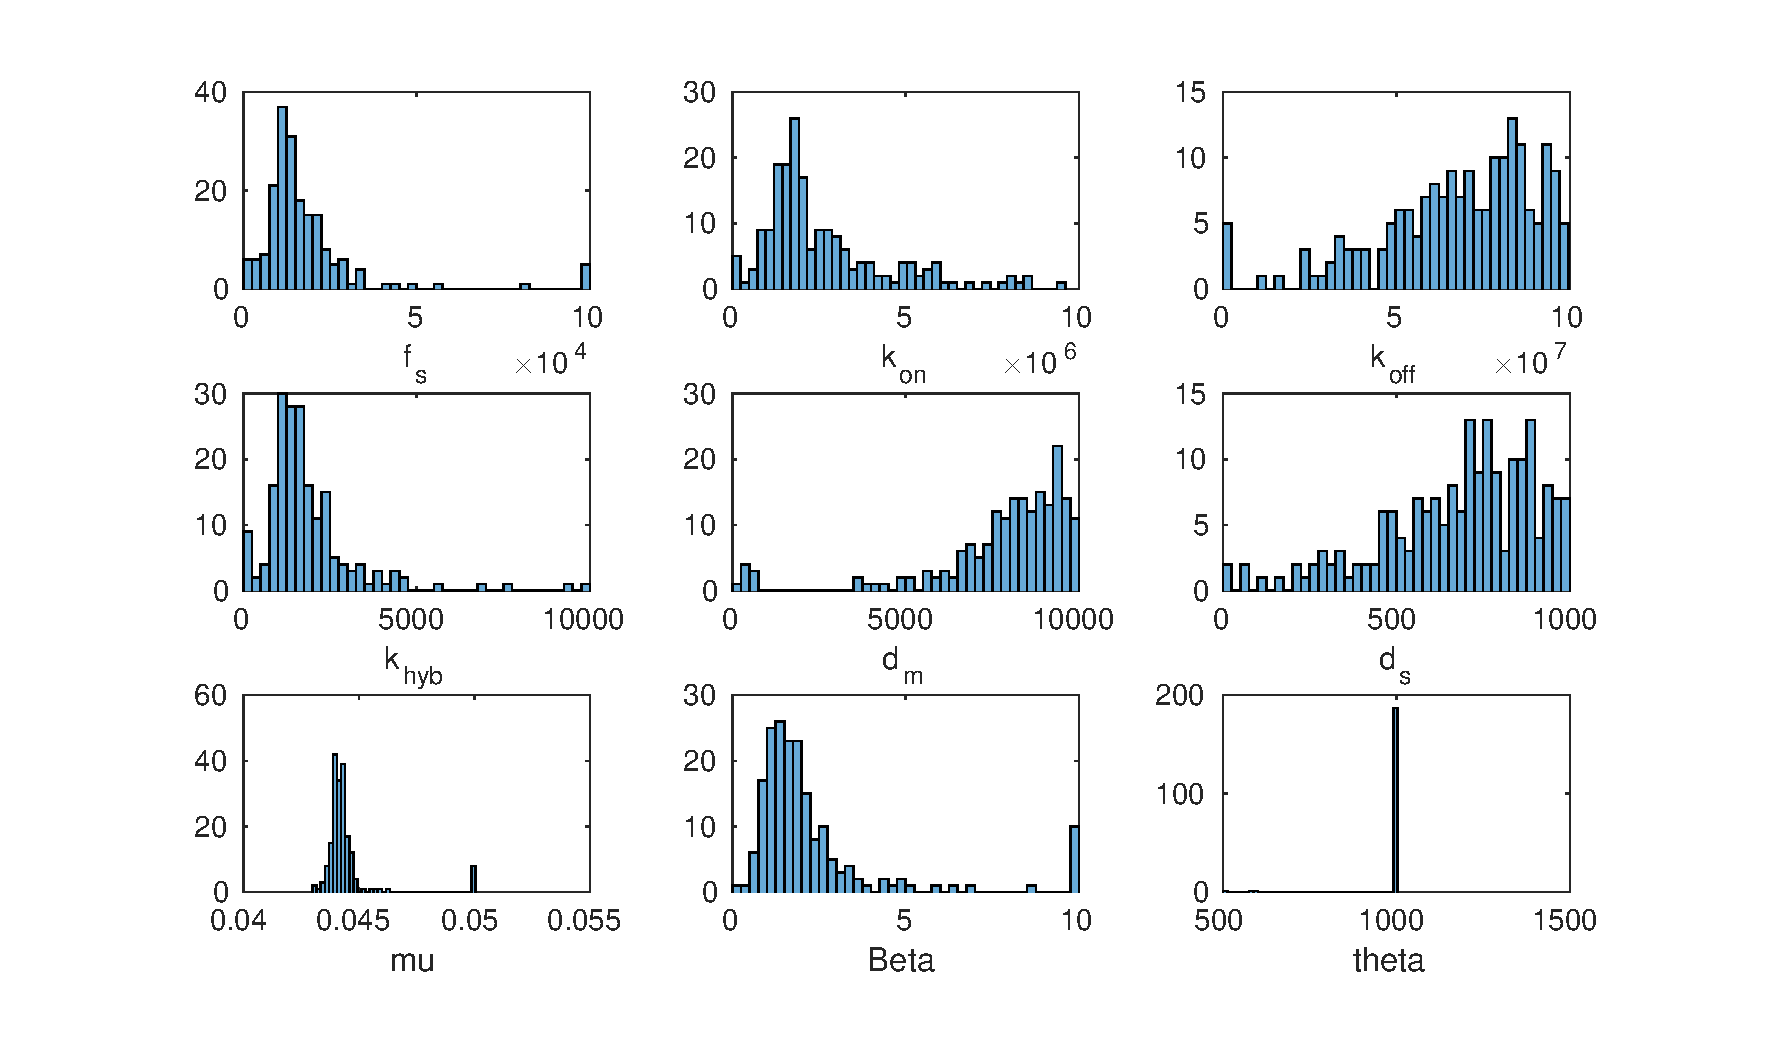
\includegraphics[scale = 0.24, clip = true, trim = 140 0 125 0]{13_9_hist}
        \caption{Histogram of estimated parameter values, found from 200 runs of the CMA-ES algorithm. Fitted to the \textit{13\_9} dataset.}
        \label{InitialResults_13_9_hist}
    \end{subfigure}
    \begin{subfigure}[c]{0.49\textwidth}
    \centering
        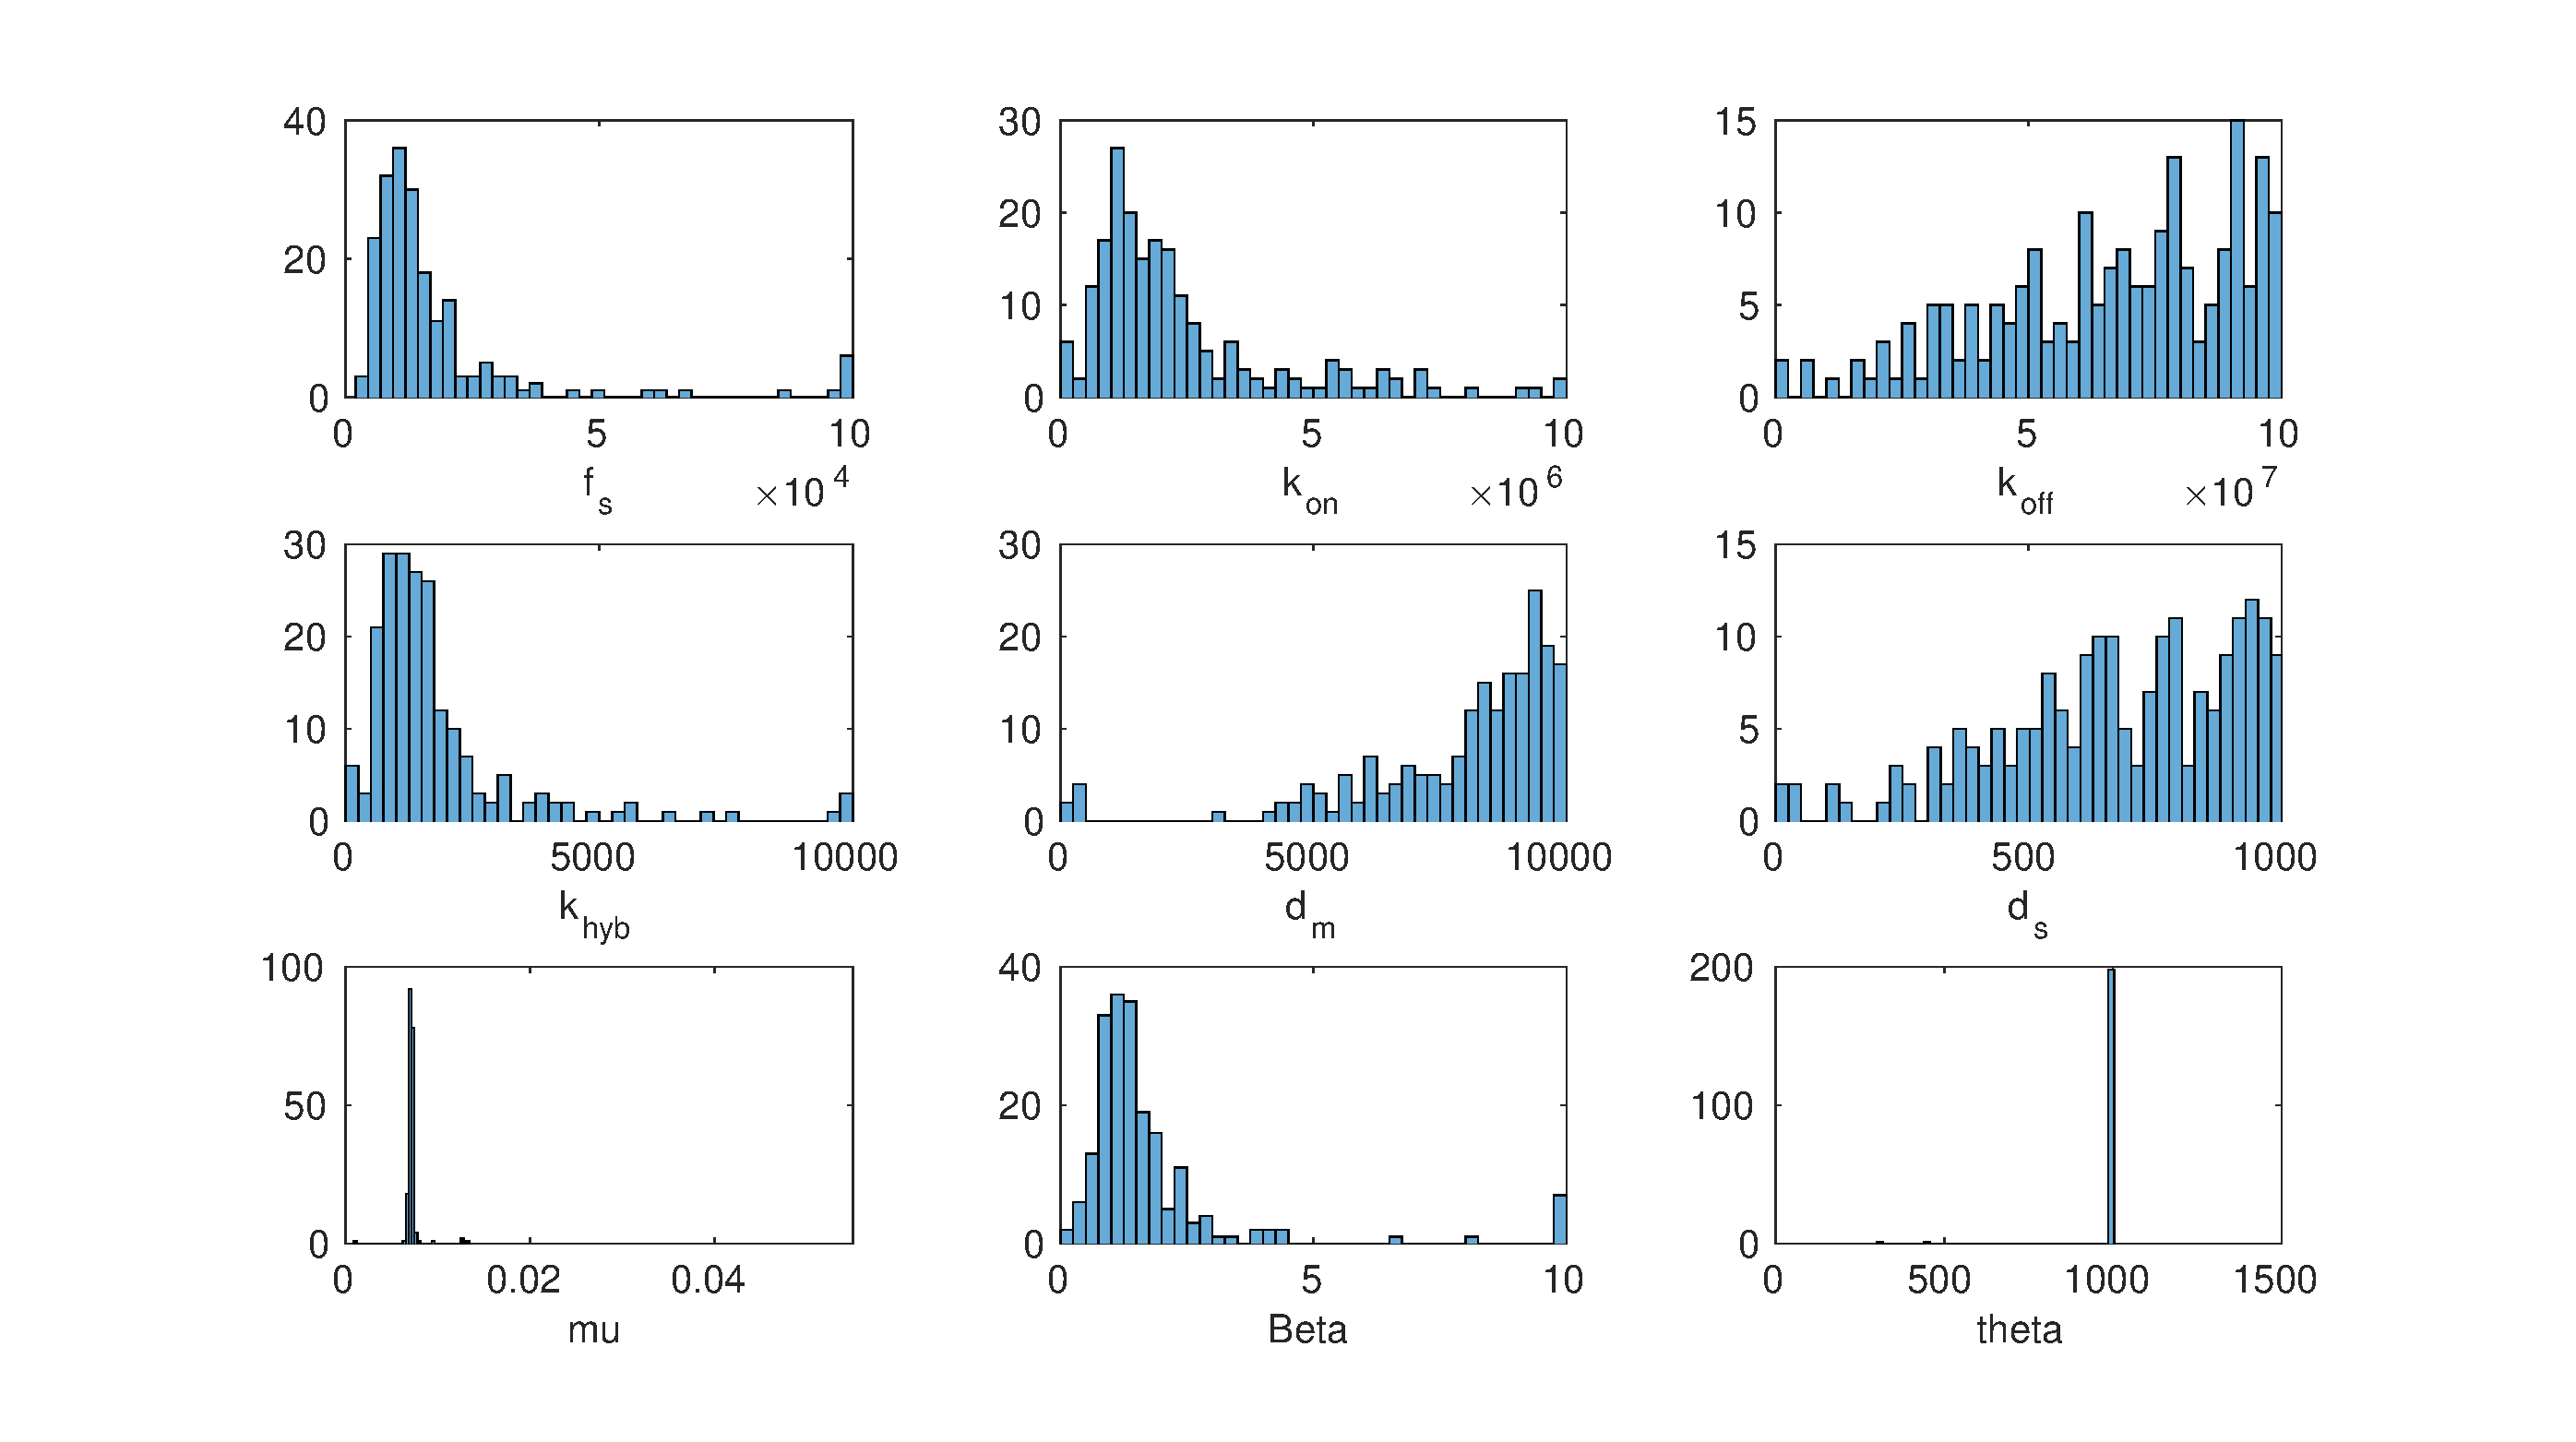
\includegraphics[scale = 0.24,clip = true, trim = 140 0 125 0]{14_7_hist}
        \caption{Histogram of estimated parameter values, found from 200 runs of the CMA-ES algorithm. Fitted to the \textit{14\_7} dataset. }
        \label{InitialResults_14_7_hist}
    \end{subfigure}

        \begin{subfigure}[c]{0.49\textwidth}
        \centering
    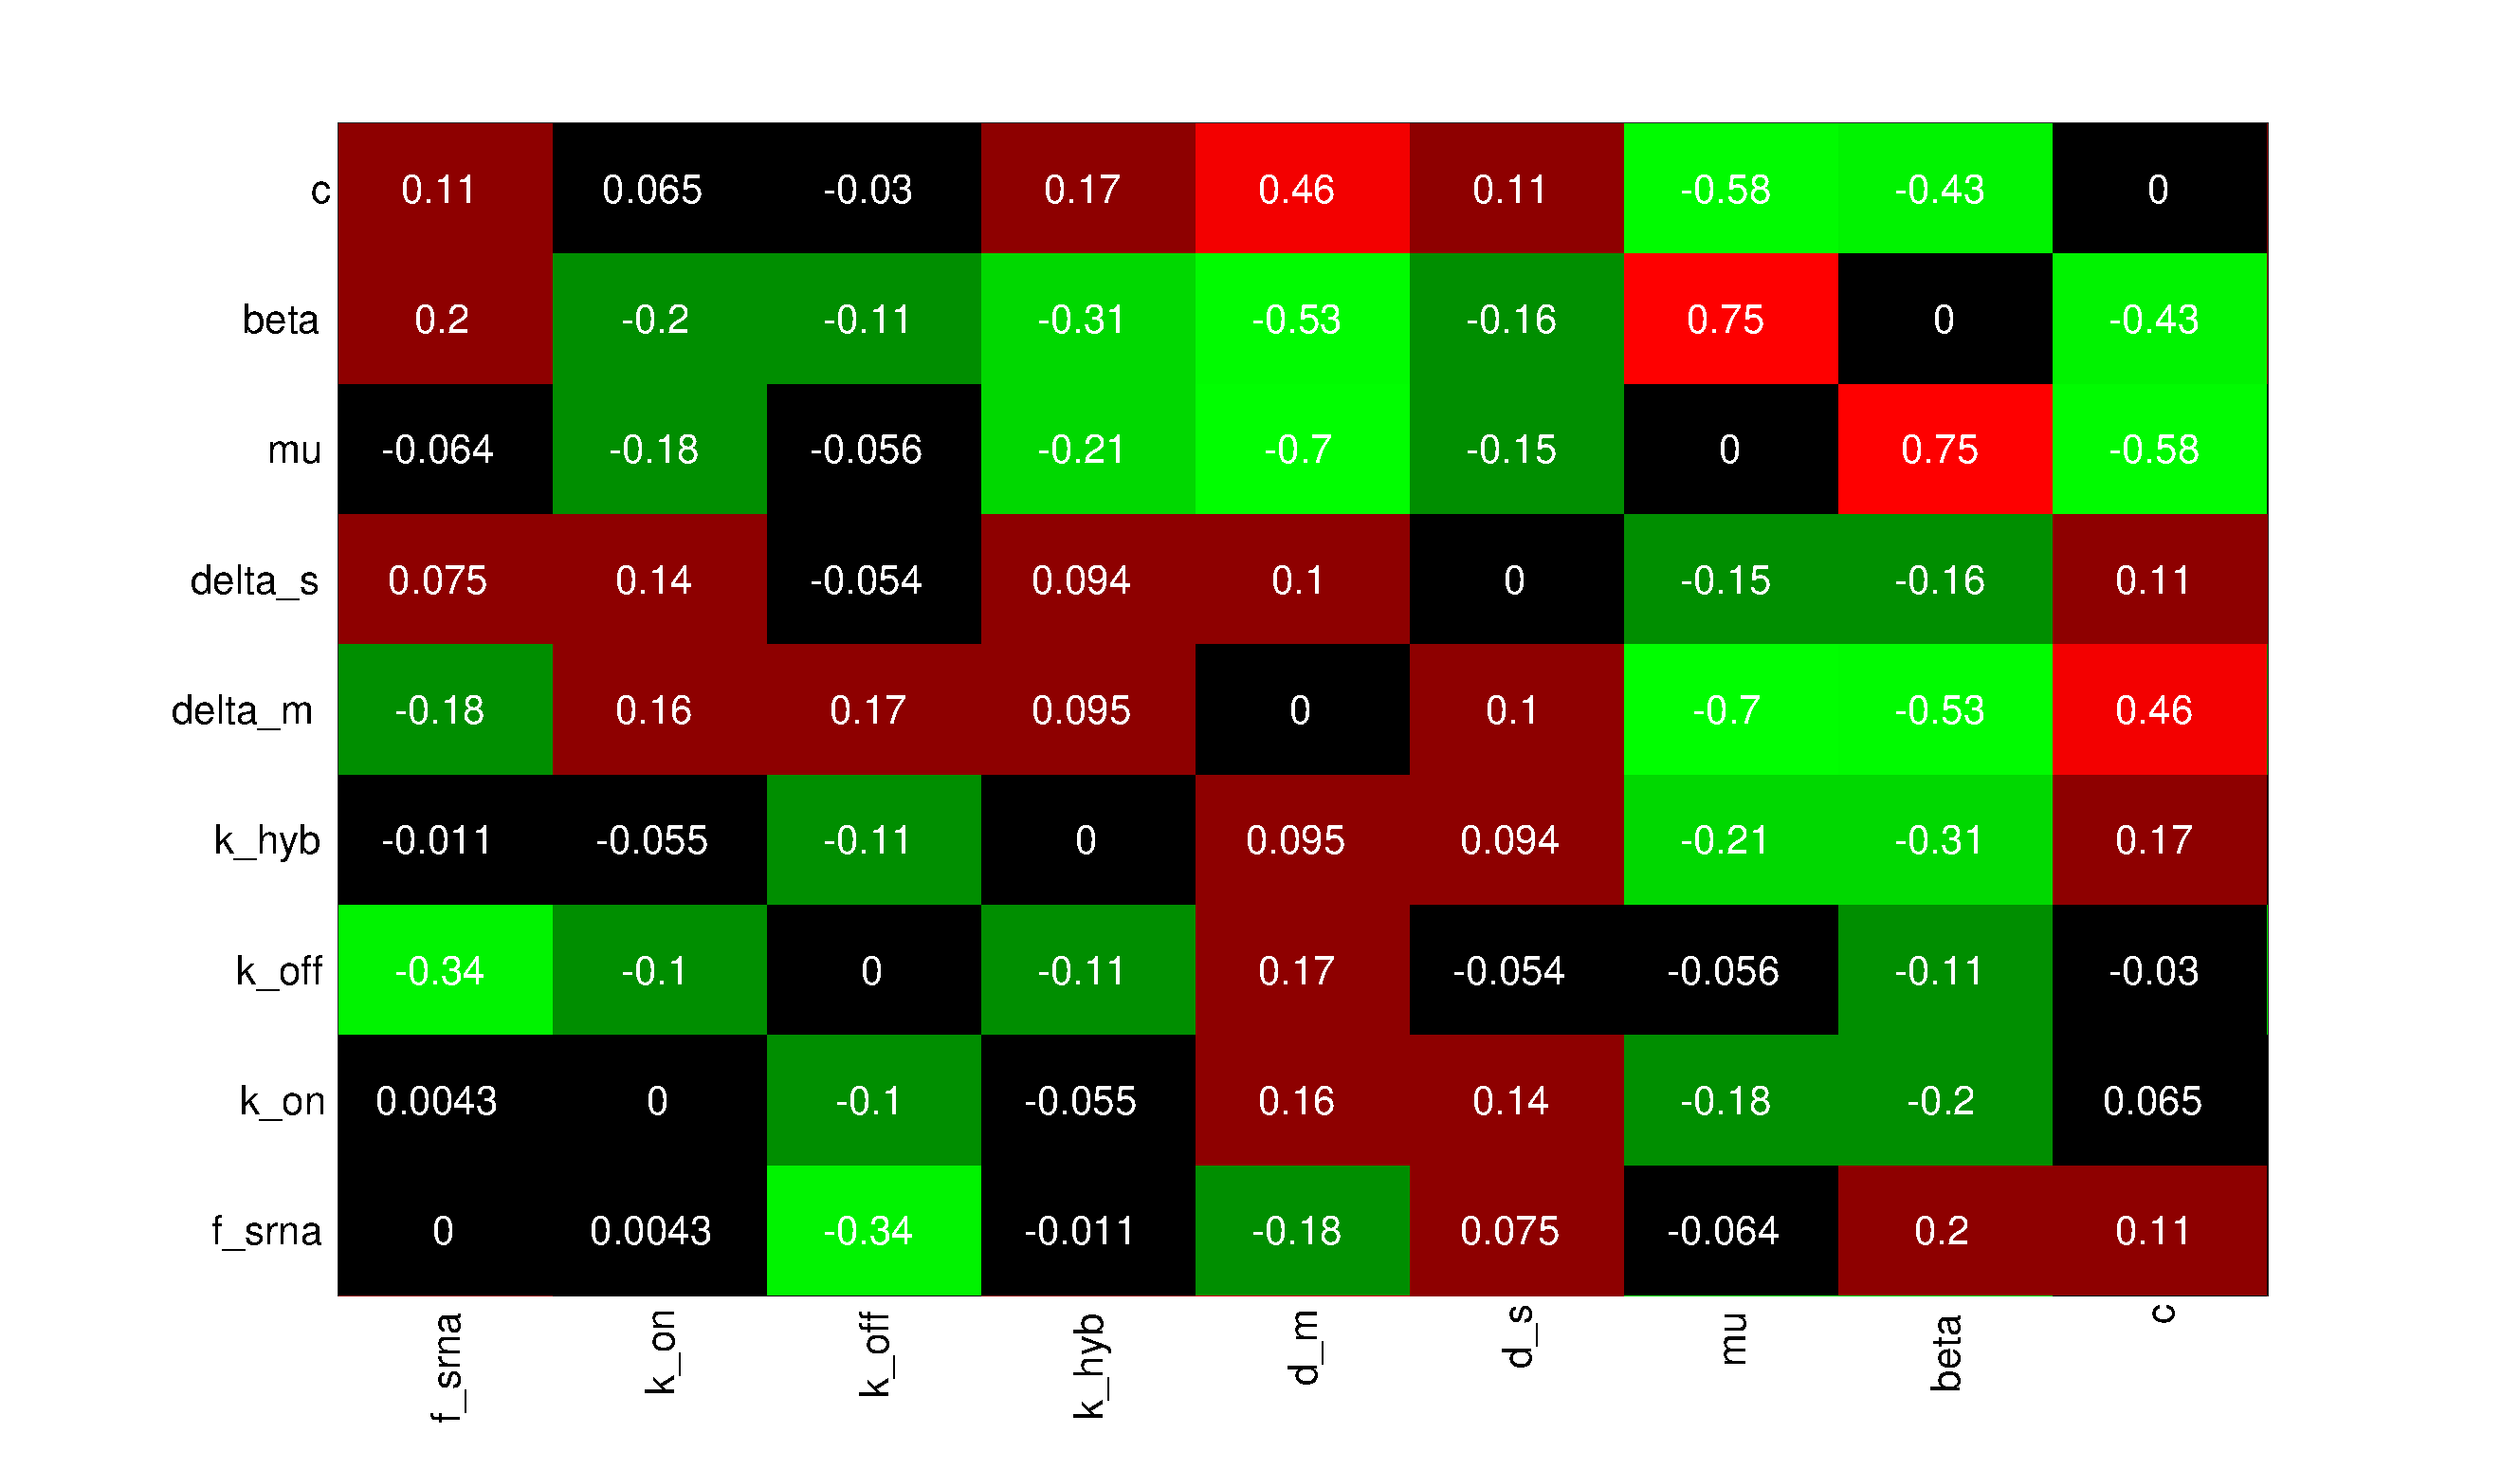
\includegraphics[scale = 0.24, clip = true, trim = 120 0 70 0]{13_9_heatmap.eps}
        \caption{Correlation matrix of estimated parameter sets, from the  \textit{13\_9} dataset. }
        \label{InitialResults_13_9_correlation}
    \end{subfigure}
    \begin{subfigure}[c]{0.49\textwidth}
    \centering
        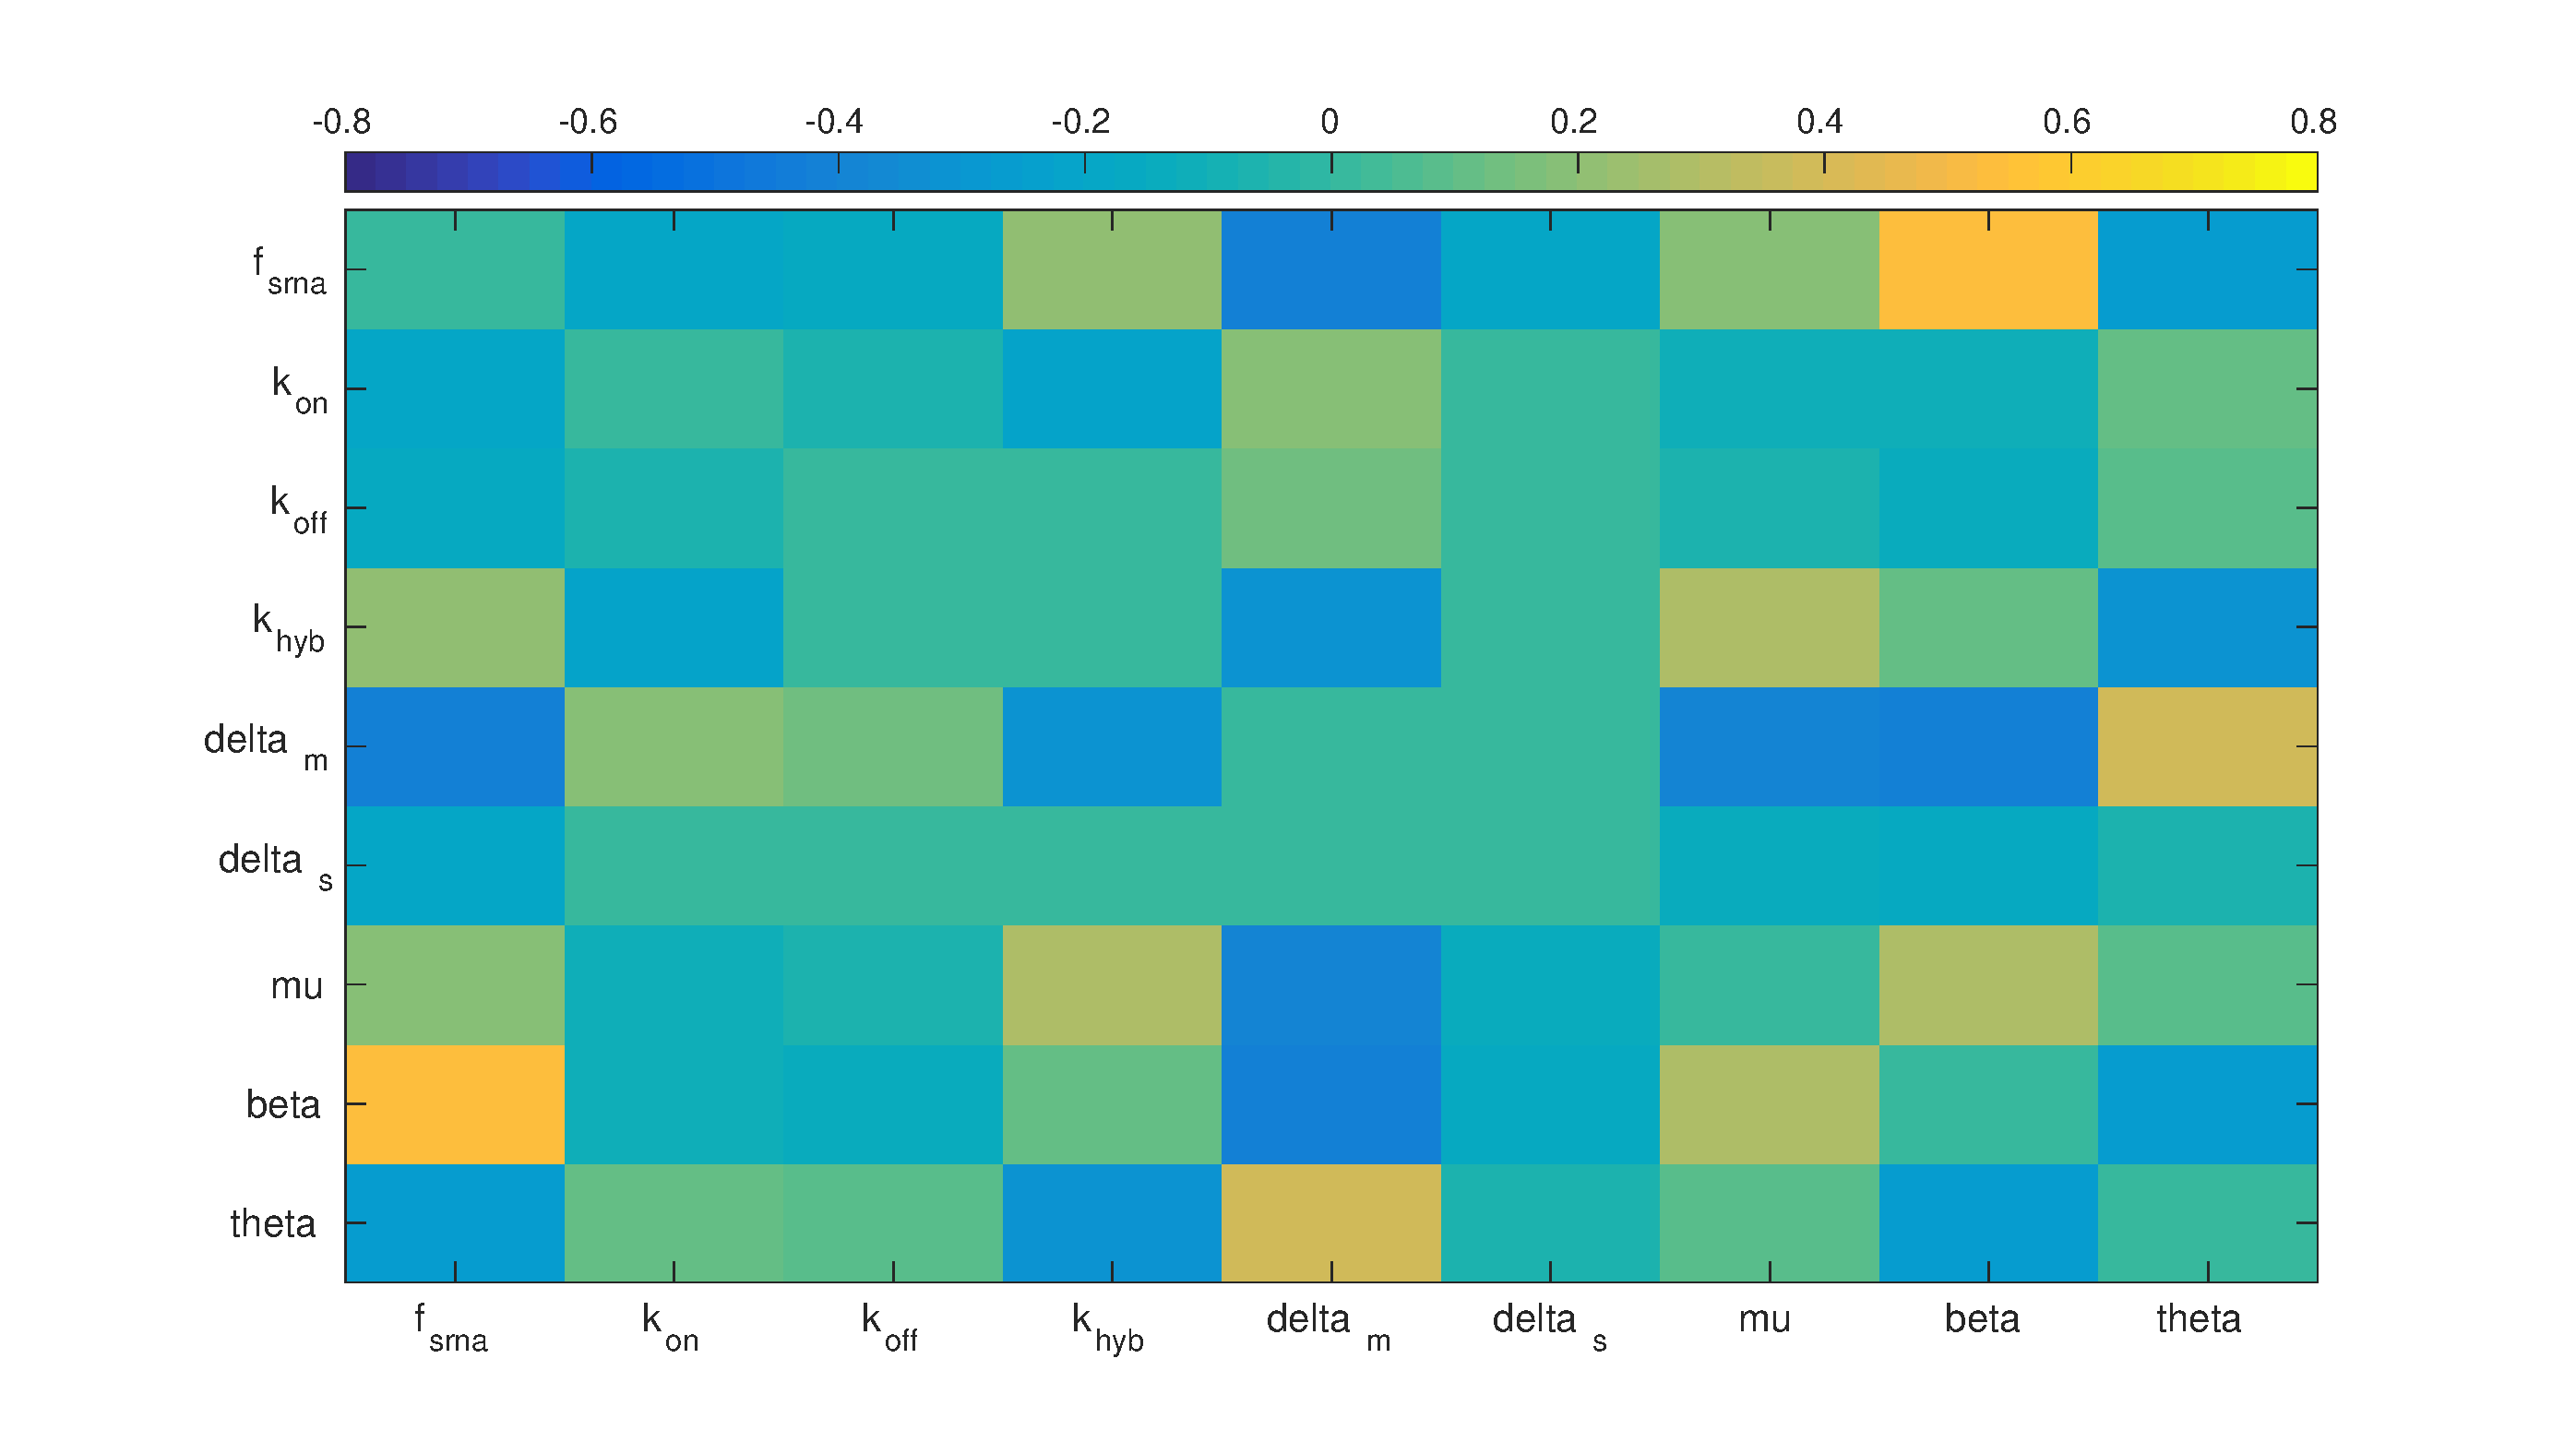
\includegraphics[scale = 0.24, clip = true, trim = 80 0 70 0]{14_7_heatmap.eps}
        \caption{Correlation matrix of estimated parameter sets, from the  \textit{14\_7} dataset.}
        \label{InitialResults_14_7_correlation}
    \end{subfigure}
    
    \begin{subfigure}[c]{0.49\textwidth}
    \centering
    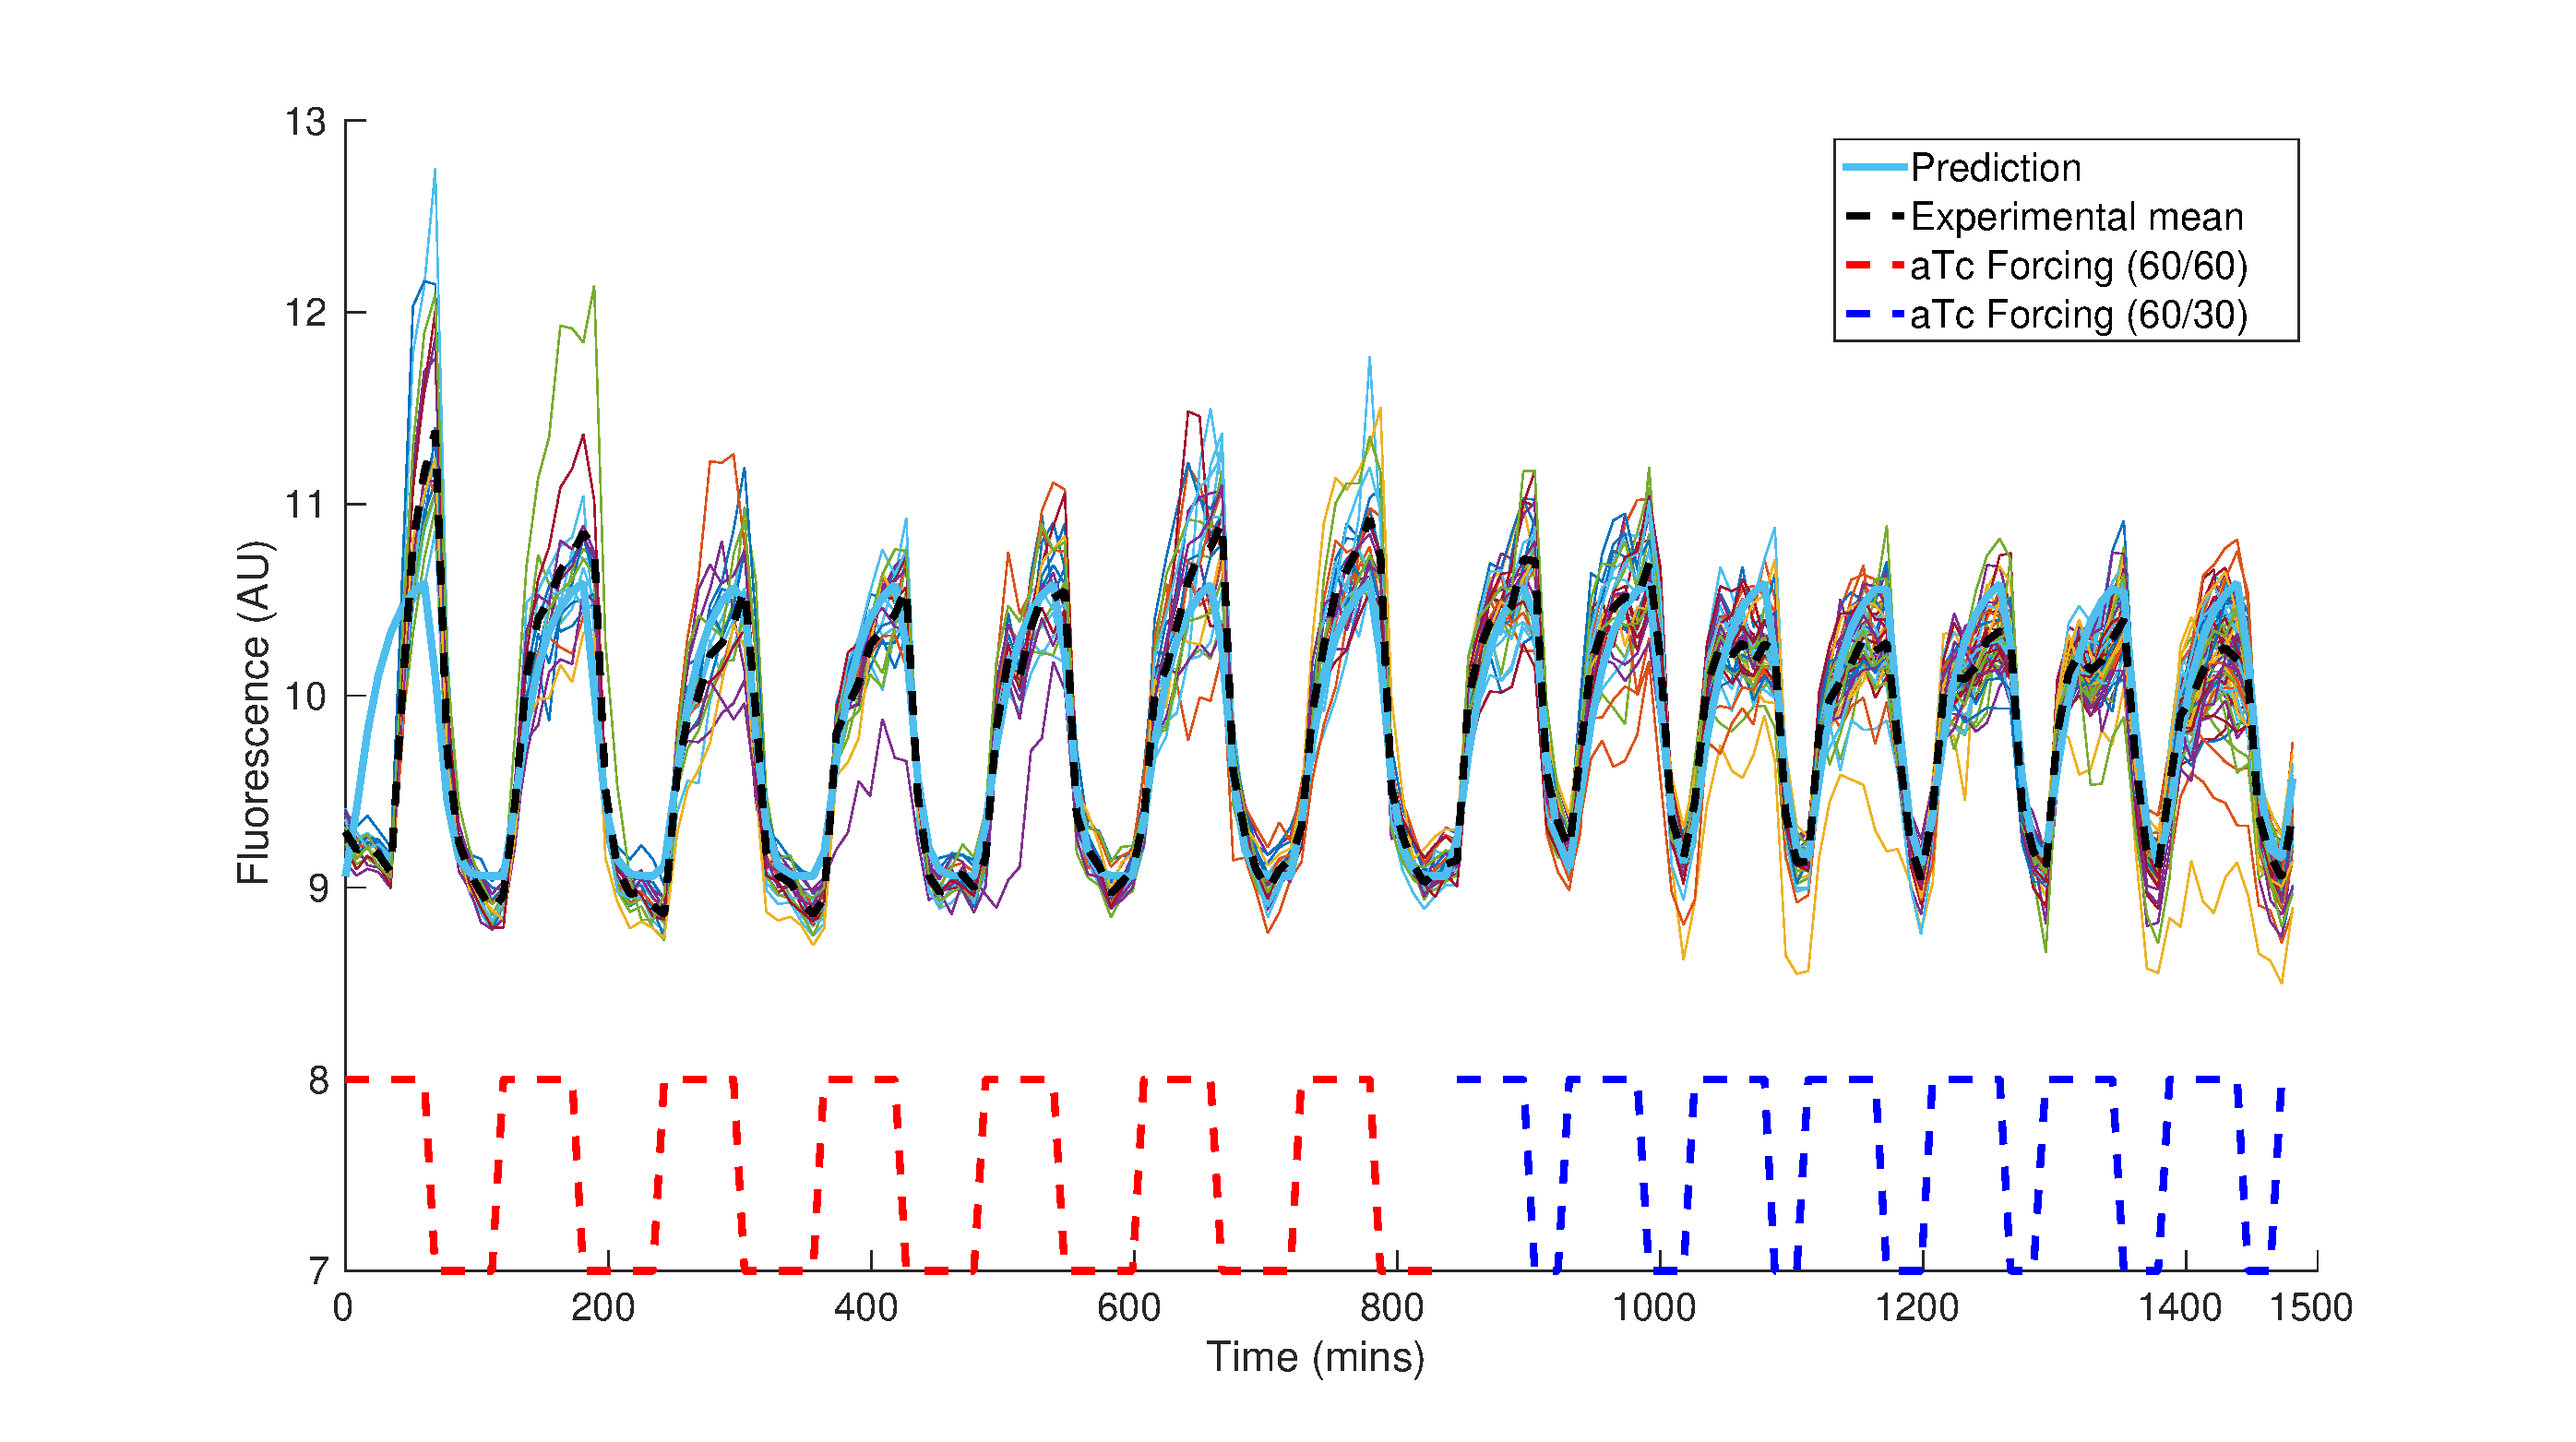
\includegraphics[scale = 0.26,clip = true, trim = 90 0 70 0]{13_9_bestPlot}
        \caption{Model prediction, using the parameter set with the smallest error value of the initial 200 found, for the \textit{13\_9} dataset.}
                \label{InitialResults_13_9_best}
    \end{subfigure}
    \begin{subfigure}[c]{0.49\textwidth}
    \centering
        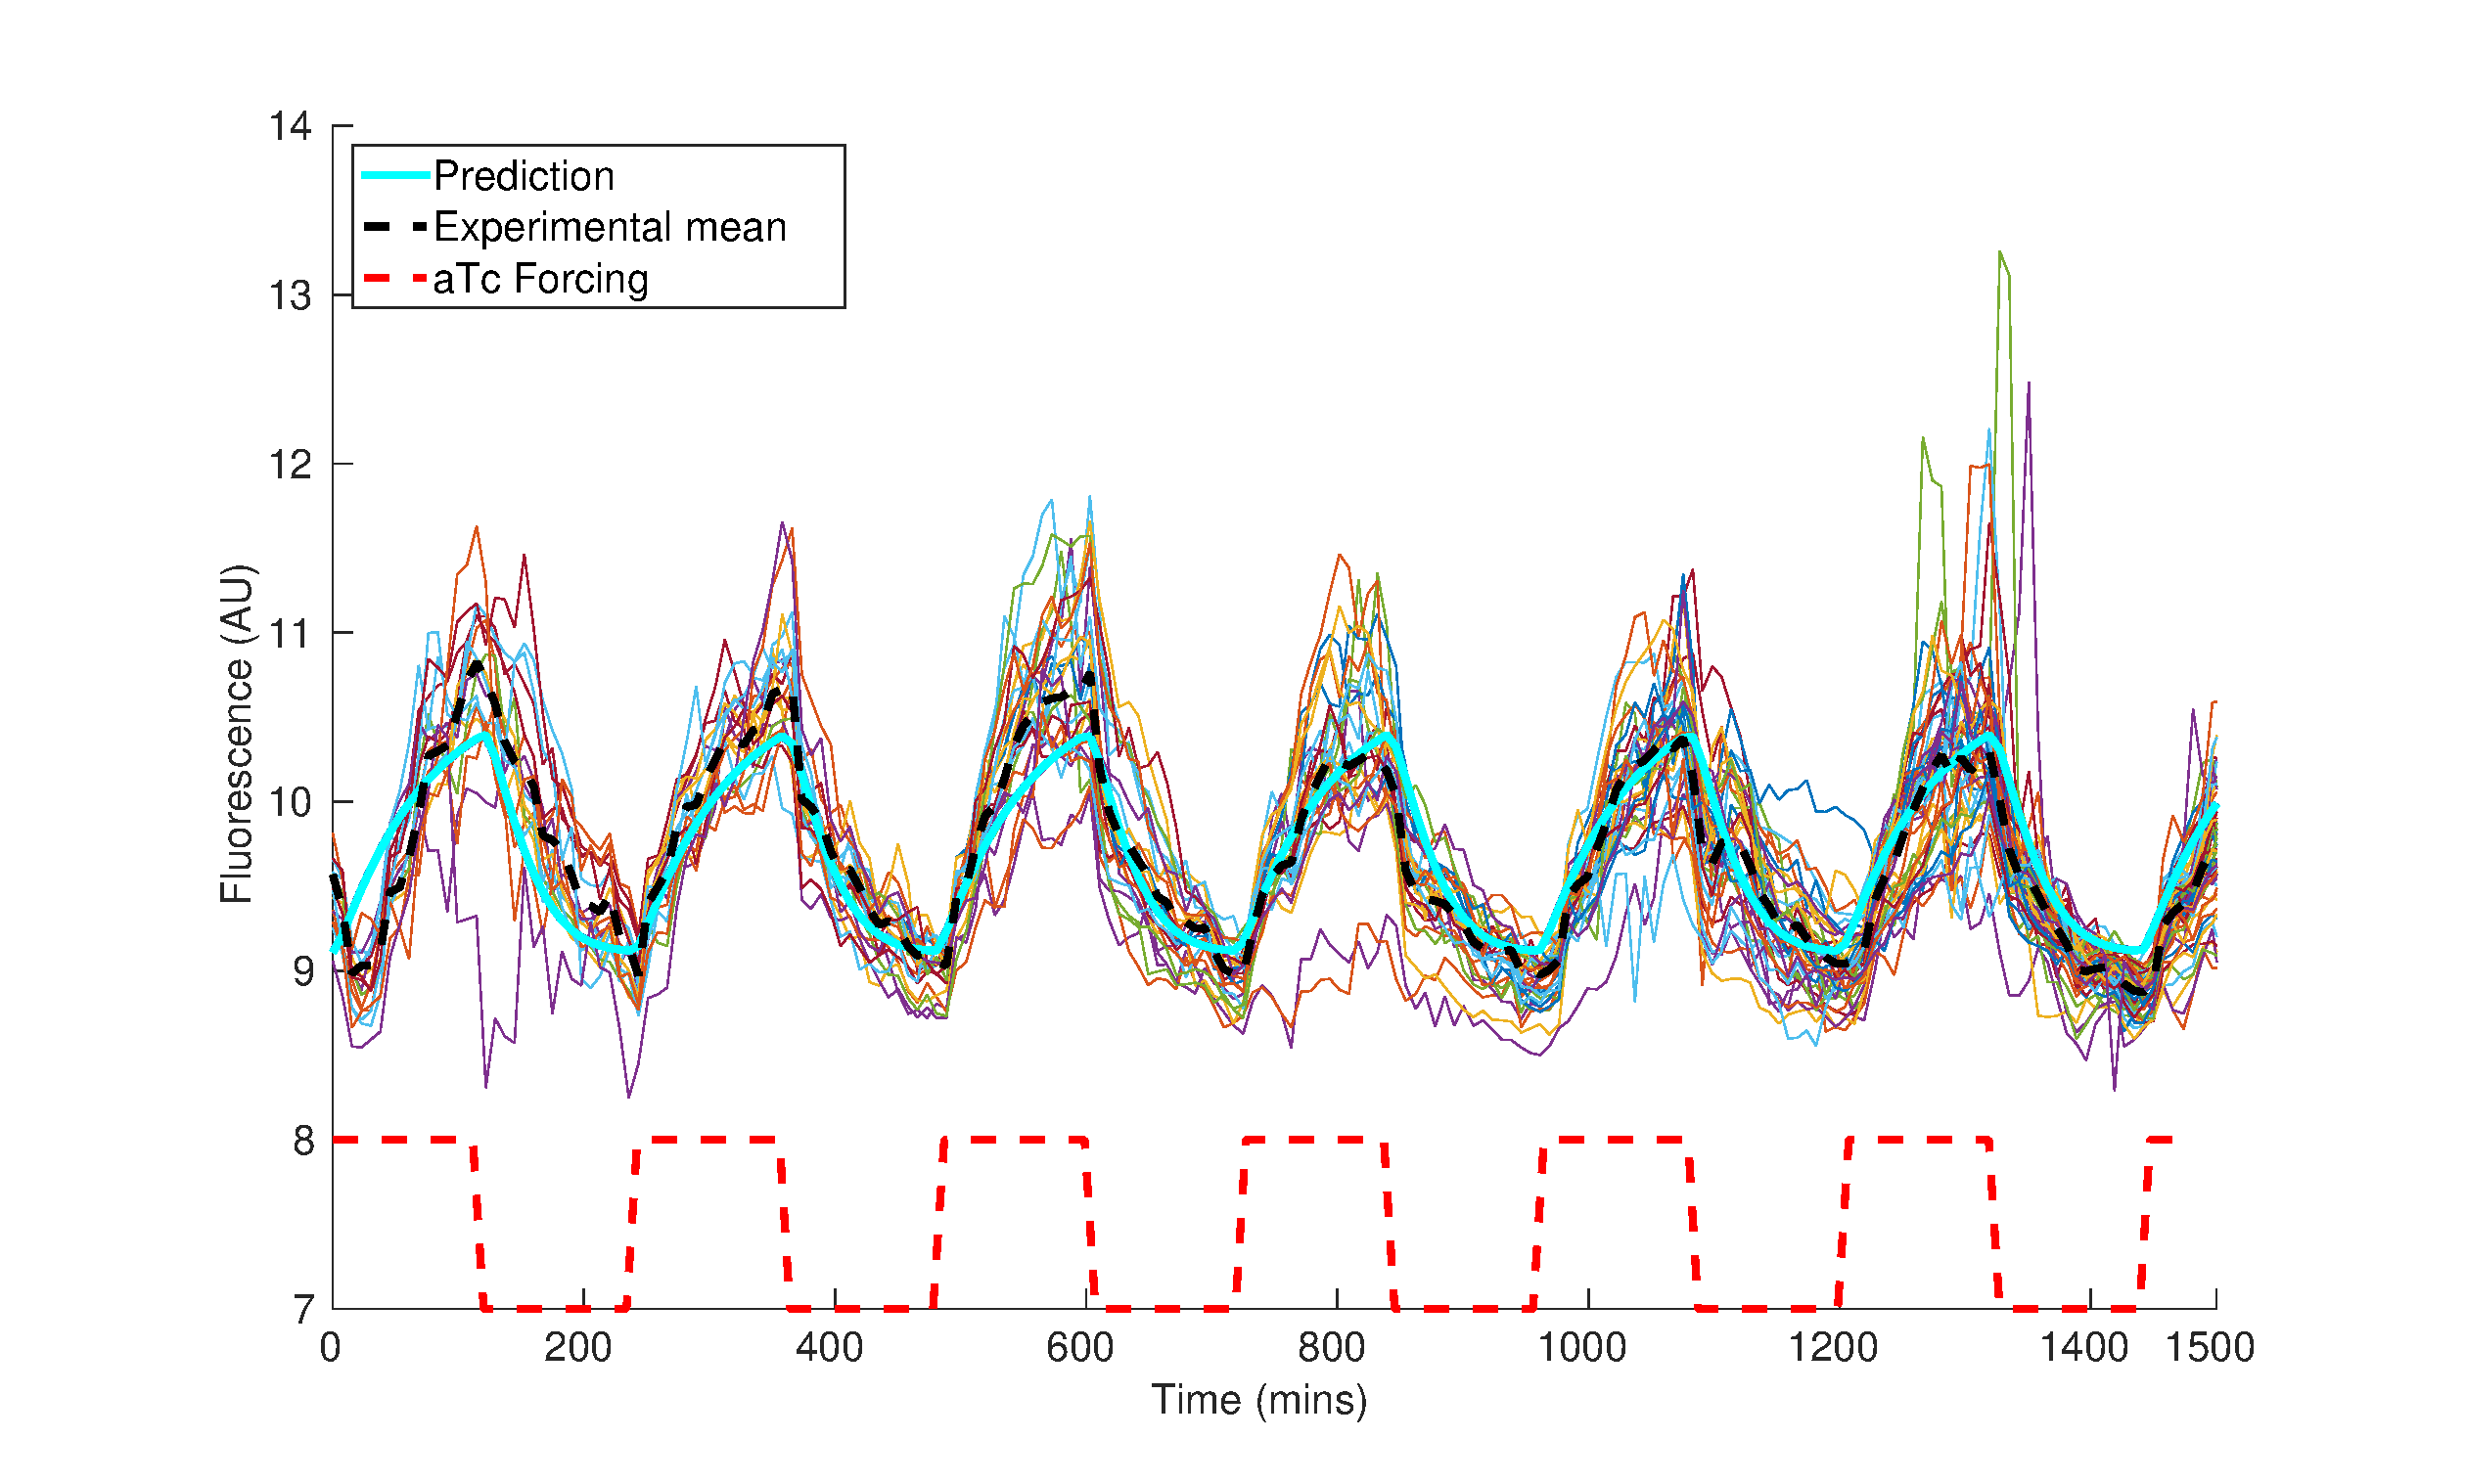
\includegraphics[scale = 0.26,clip = true, trim = 90 0 70 0]{14_7_bestPlot}
        \caption{Model prediction, using the parameter set with the smallest error value of the initial 200 found, for the \textit{14\_7} dataset.}
        \label{InitialResults_14_7_best}
    \end{subfigure}
    \caption{Parameter estimates, inter-parameter correlation values, and model predictions for the \textit{13\_9} and \textit{14\_7} datasets. Note that in the model predictions, aTc forcing is shown - IPTG concentration is constant at a level which saturates the cell's response. The forcing curve's height is schematic - aTc concentration is switched between off, and a level which saturates the cell's response.}
\label{InitialResults}
\end{figure*} 
 

% NEW SUBSECTION

\subsection{Initial Parameter Estimates}
\label{Initial Parameter Estimates}


 We begin by fitting each dataset individually, by choosing 200 parameter sets uniformly distributed over our initial parameter bounds and running the CMA-ES starting from them. Results are shown in Figs. \ref{InitialResults}, \ref{hist_f}. Figs. \ref{InitialResults_13_9_best}, \ref{InitialResults_14_7_best}  demonstrate that the model is capable of quantitatively capturing the data. However, histograms of estimated parameter values found from fitting the above 200 sets indicate many parameter estimates are not tightly constrained, taking values right across the initial bounding range specified - in particular, $k_\mathrm{off}$, $\delta_{m}$ and $\delta_{s}$ are very weakly constrained, with substantial numbers of runs constrained only by the initial bounding box. By contrast, some parameter estimates ($\mu$ in particular) are much tighter. $\Theta$ appears tightly constrained, but many of the estimated values are close to the upper bound set, and must be treated with caution.

Figs. \ref{InitialResults_13_9_correlation}, \ref{InitialResults_14_7_correlation} show correlation matrices between parameter sets, computed by viewing each of the estimated parameter sets as a sample from a multivariate random variable. An element of the correlation matrix $R_{ij}$ is then the correlation co-efficient between the $i^\mathrm{th}$ and $j^\mathrm{th}$ random variable - or, in our case, the $i^\mathrm{th}$ and $j^\mathrm{th}$ parameters. These correlation matrices indicate that there are spaces of parameters within which the fitness function remains approximately constant - for example, in both datasets there exists of positive correlation between values of $\mu$ and $\beta$. Referring to \eqref{eq:p}, this makes heuristic sense - the two parameters may have similar effects on model predictions, and may be able to co-vary in such a way as to leave the model prediction unchanged. Biologically, an increased production rate of GFP is being balance by an increased dilution rate. 
The results suggest a fitness landscape relatively flat to perturbations in certain combinations of parameters, and indicate we may have difficulty obtaining unique estimates of the model parameters.
 
 We can test the predictive ability of our model by cross validating, either by taking the parameter values found in the fitting of one dataset and using them to give model predictions for another, or only fitting part of a single dataset and predicting the rest.  We begin by fitting to only the data for the first forcing period in \textit{13\_9}, and then predicting the full time series. Results are shown in Fig. \ref{CrossValidation_1}, for the parameter set giving the lowest error on the training data. We see the prediction is very similar to that obtained by fitting to the full dataset (Fig. \ref{InitialResults_13_9_best}). Next, we take the parameter values giving the best fit for the  \textit{13\_9} dataset and use them to predict the \textit{14\_7} dataset, and vice versa. Results are shown in Figs. \ref{CrossValidation_2}, \ref{CrossValidation_3}.
Though the predictions are reasonable, they are substantially worse than the predictions for the data they were trained on. One reason for this may be that parameter values will vary between experimental runs \cite{Hu2015}. We can also fit to both datasets combined, by extending \eqref{eq:min} to a sum over multiple datasets. Results are shown in Appendix \ref{Bothdatasetfitting}. We are unable to achieve error values as low as those found when fitting individual datasets. In addition, we do not see a tightening of the estimates on our parameters, as we might expect from including the additional data. Instead, many parameter estimates remain spread across the initial bounding region. We also note that all three of the cases considered (\textit{13\_9}, \textit{14\_7}, both) see a shift in the estimated value of $\mu$.
 
 \begin{figure}[h]	
 	\begin{subfigure}[h]{0.49\textwidth}
    \centering
        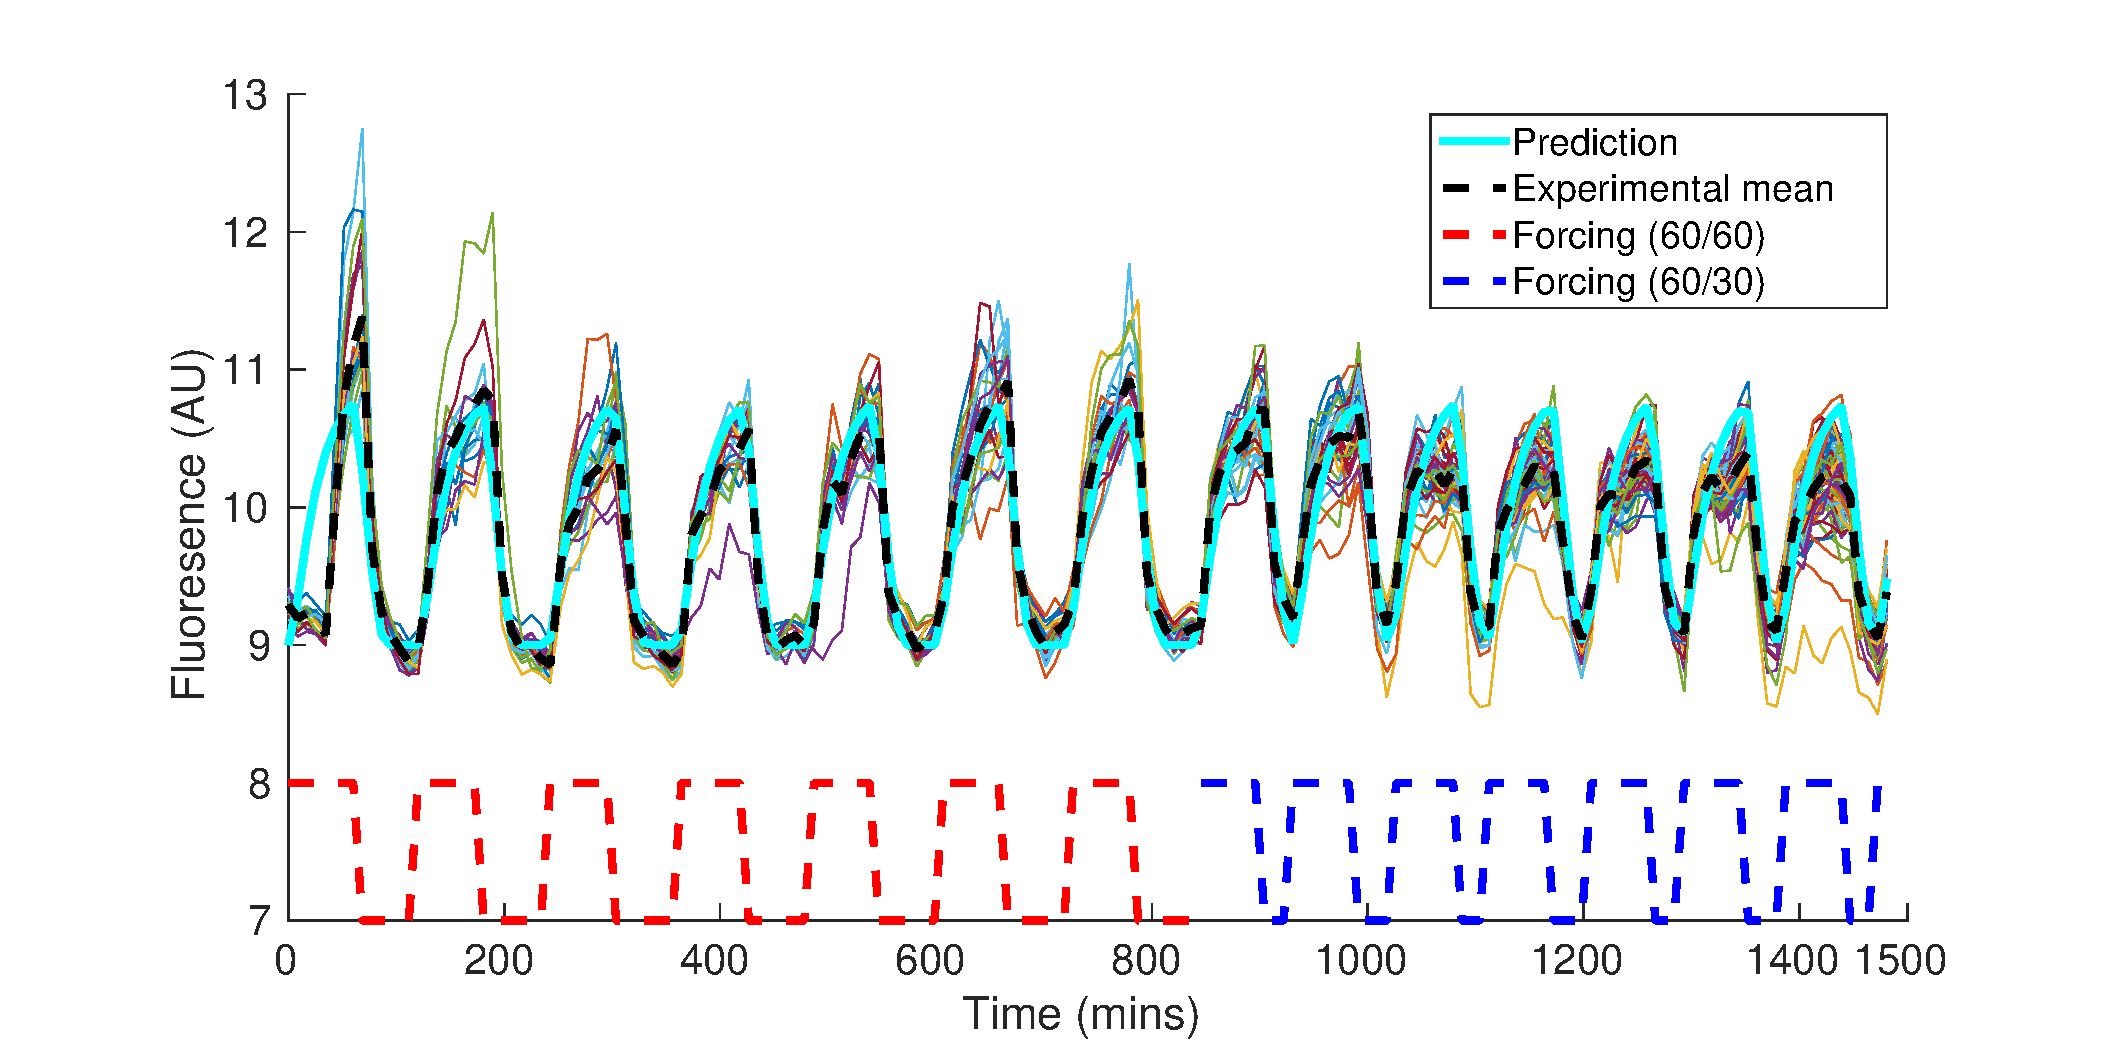
\includegraphics[scale = 0.29,clip = true, trim = 82 0 70 0]{13_9_partial_data_13_9_pred}
        \caption{Model trained on \textit{13\_9}  60/60 data only, full prediction}
        \label{CrossValidation_1} 
    \end{subfigure}
	\begin{subfigure}[h]{0.49\textwidth}
    \centering
        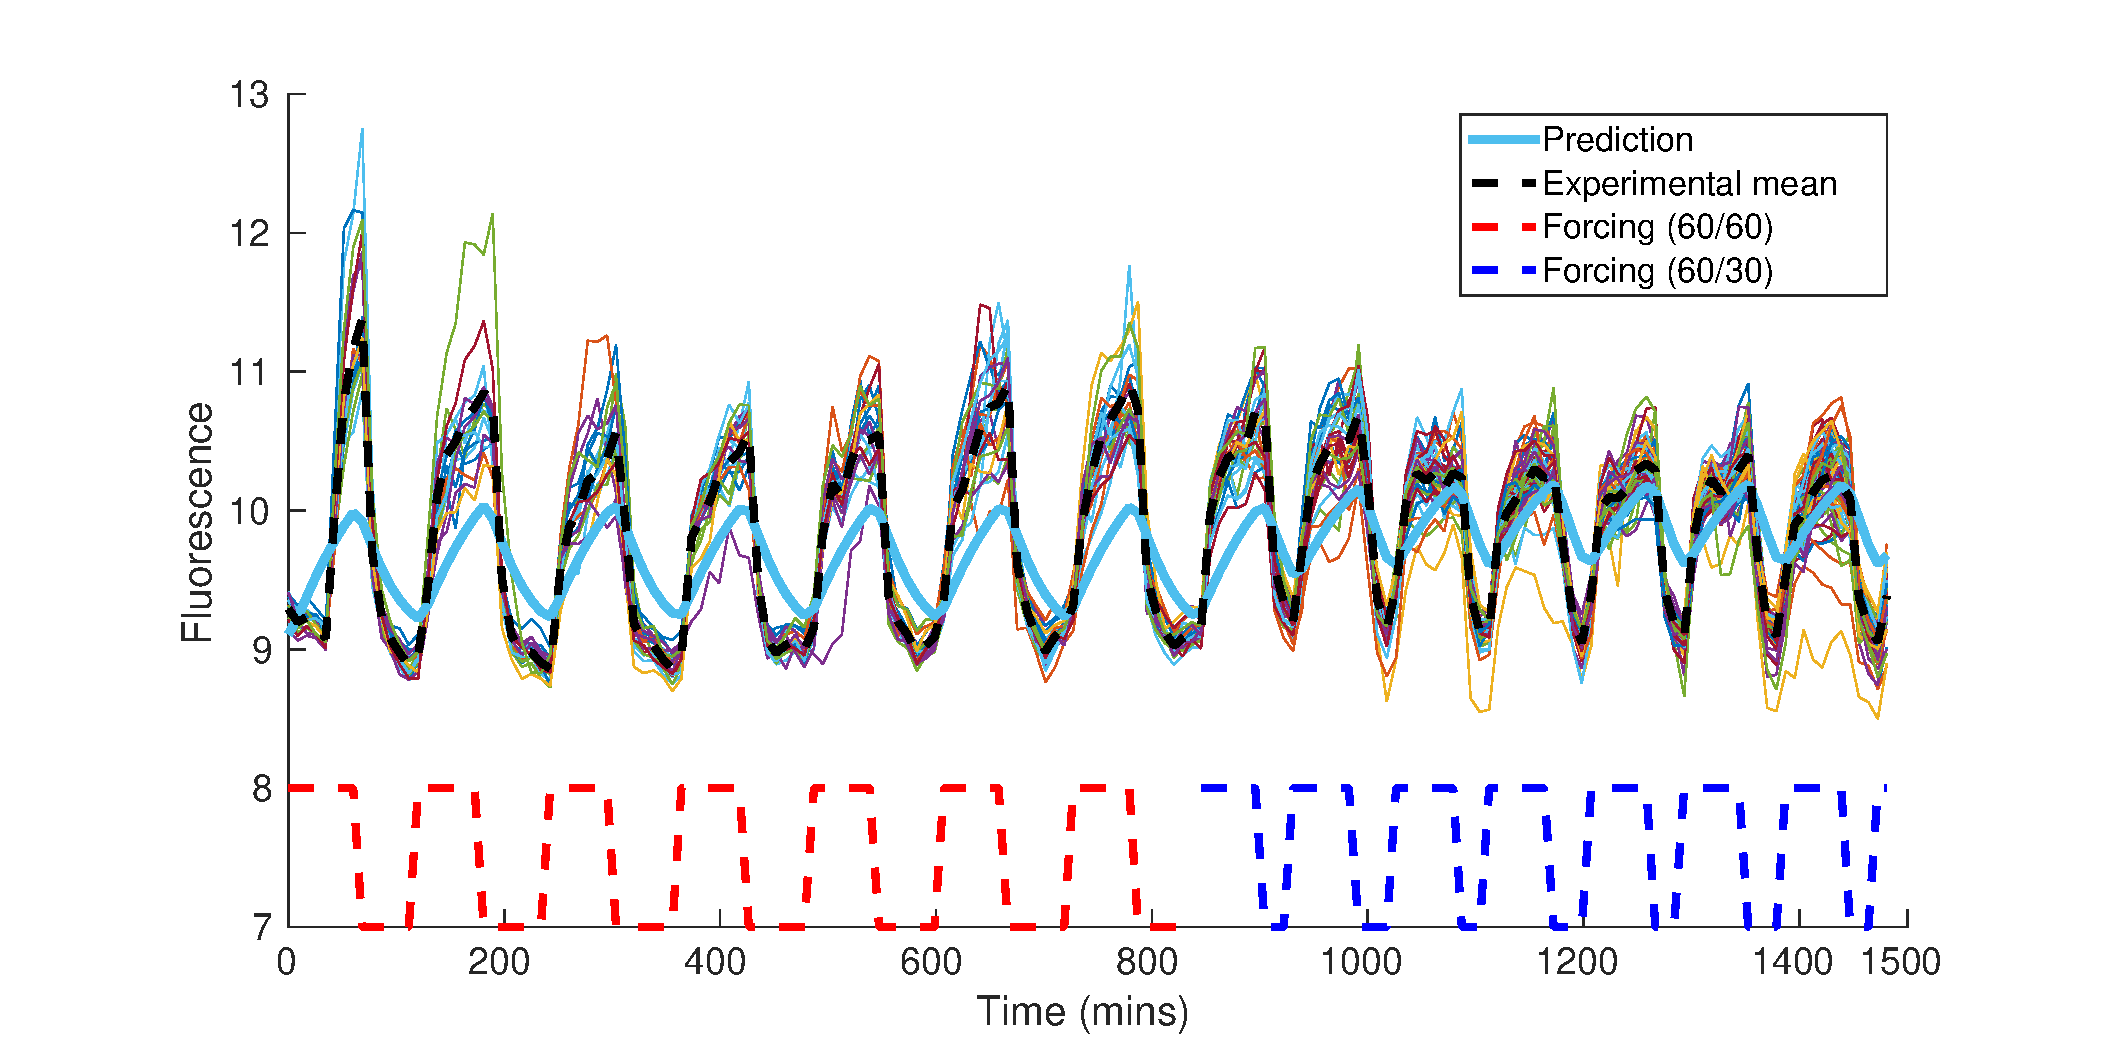
\includegraphics[scale = 0.3,clip = true, trim = 87 0 70 0]{14_7_pred_13_9_data}
        \caption{\textit{14\_7} prediction \textit{13\_9} data}
        \label{CrossValidation_2} 
    \end{subfigure}
    \begin{subfigure}[h]{0.49\textwidth}
    \centering
        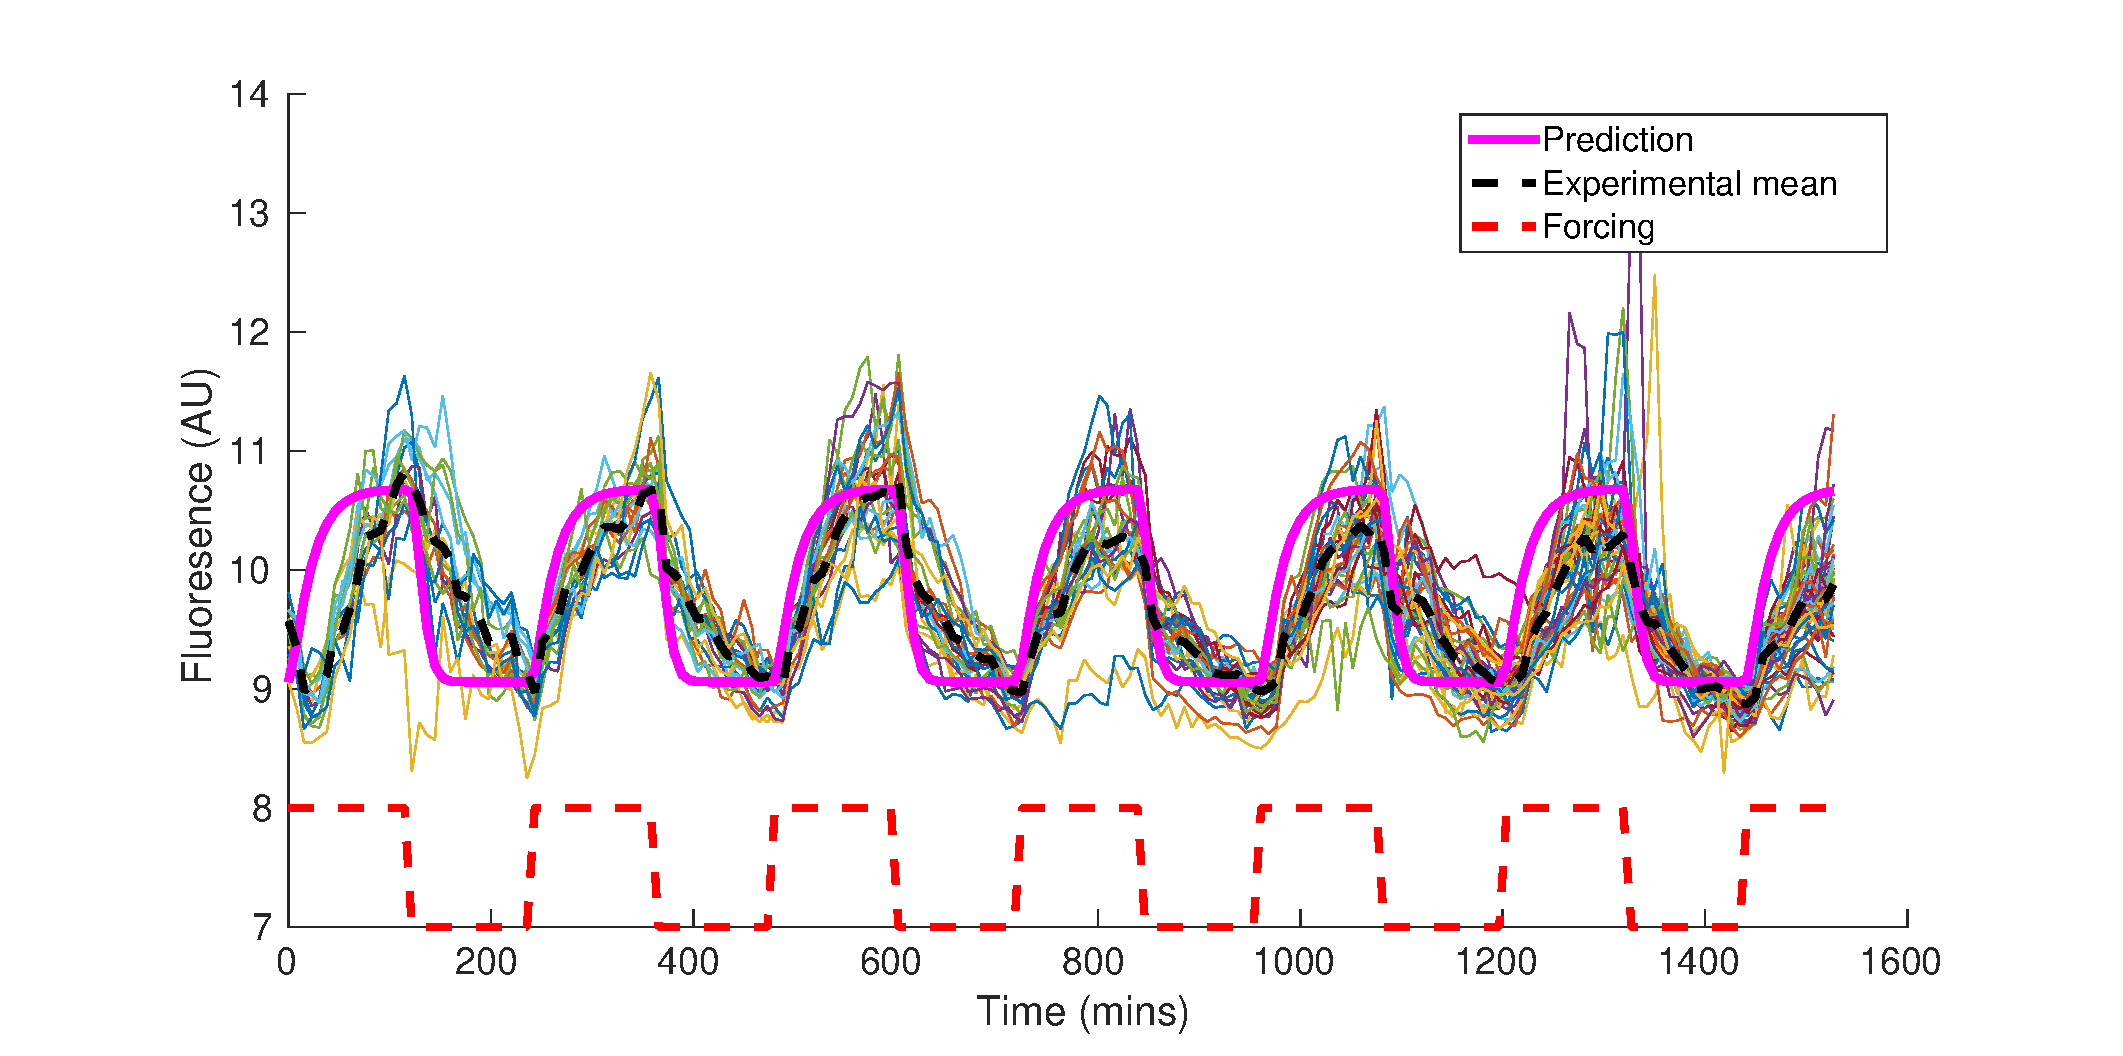
\includegraphics[scale = 0.3,clip = true, trim = 87 0 70 0]{13_9_pred_14_7_data}
        \caption{\textit{13\_9} prediction \textit{14\_7} data}
                \label{CrossValidation_3} 
    \end{subfigure}
    \caption{Cross validating data by taking parameter estimates from one dataset, and using them to predict another. \ref{CrossValidation_1} shows model predictions for the full \textit{13\_9} dataset, when only trained on the first forcing period data. \ref{CrossValidation_2}, \ref{CrossValidation_3} show model predictions for fitting to one dataset, and predicting the other.}
\label{CrossValidation}   
\end{figure}

 Taken together, these results suggest that simply performing a least squares fit on the available data will not give unique parameter estimates. In the following sections we investigate why this might be.
 
 \begin{figure*}[!t]
% ensure that we have normalsize text
\tiny
% Store the current equation number.
\setcounter{MYtempeqncnt}{\value{equation}}
% Set the equation number to one less than the one
% desired for the first equation here.
% The value here will have to changed if equations
% are added or removed prior to the place these
% equations are referenced in the main text.
\setcounter{equation}{11}
\begin{align}
\label{eq:m_fixed}  
m &= \frac{1}{{2 k_{\text{on}} \left(\mu +\delta _m\right)
   \left(k_{\text{hyb}}+\delta _m\right)}}
   \Bigg(\sqrt{2 (\text{am}+\text{as}) k_{\text{on}} \left(\mu +\delta _m\right) \left(\mu +\delta _s\right) \left(k_{\text{hyb}}+\delta _m\right)
   \left(k_{\text{hyb}}+k_{\text{off}}+\delta _m\right)+(\text{am}-\text{as})^2 k_{\text{on}}^2 \left(k_{\text{hyb}}+\delta _m\right){}^2+\left(\mu +\delta _m\right){}^2
   \left(\mu +\delta _s\right){}^2 \left(k_{\text{hyb}}+k_{\text{off}}+\delta _m\right){}^2} \\ \nonumber  
 &- (\text{am}-\text{as}) k_{\text{on}} \left(k_{\text{hyb}}+\delta
   _m\right)+\left(\mu +\delta _m\right) \left(\mu +\delta _s\right) \left(k_{\text{hyb}}+k_{\text{off}}+\delta _m\right)\Bigg)
\end{align}
\begin{align}
\label{eq:c_fixed}
c &= \frac{k_{\text{hyb}}}{2 k_{\text{on}} \left(\mu +\delta
   _m\right) \left(k_{\text{hyb}}+\delta _m\right){}^2}
   \Bigg( \sqrt{2 (\text{am}+\text{as}) k_{\text{on}} \left(\mu +\delta _m\right) \left(\mu +\delta _s\right) \left(k_{\text{hyb}}+\delta _m\right)
   \left(k_{\text{hyb}}+k_{\text{off}}+\delta _m\right)+(\text{am}-\text{as})^2 k_{\text{on}}^2 \left(k_{\text{hyb}}+\delta _m\right){}^2+\left(\mu +\delta _m\right){}^2
   \left(\mu +\delta _s\right){}^2 \left(k_{\text{hyb}}+k_{\text{off}}+\delta _m\right){}^2} \\ \nonumber
   &+(\text{am}+\text{as}) k_{\text{on}} \left(k_{\text{hyb}}+\delta
   _m\right)+\left(\mu +\delta _m\right) \left(\mu +\delta _s\right) \left(k_{\text{hyb}}+k_{\text{off}}+\delta _m\right) \Bigg)
\end{align}
% Restore the current equation number.
\setcounter{equation}{\value{MYtempeqncnt}}
% IEEE uses as a separator
\hrulefill
% The spacer can be tweaked to stop underfull vboxes.
\vspace*{4pt}
\end{figure*}
 
 \subsection{Parameter Estimability}
\label{Parameter Estimability}
 
 There are two main reasons why a parameter may not be estimable \cite{Mclean2012,Yao2003, Beck}: Model predictions may be insensitive to the value of a particular parameter, or the effects of varying one parameter on model predictions may be highly correlated with the effects of varying several others.
 
These problems may stem from structural inadequacies in the model (often termed \textit{structural identifiability}), in which two different parameter sets can give identical model predictions \cite{Jimenez-Hornero2008,Grewal1976 }. If this is the case, no amount of experimental data will allow us to estimate parameters, and we must consider reformulating the model. \footnote{A simple example of a structurally non - identifiable model is $y = \beta_{1}\beta_{2}x$, where we are given data $(x,y)$, and asked to estimate parameters $\beta_{1}$ and $\beta_{2}$ - we can see that, in principle, only the product $\beta_{1}\beta_{2}$ can ever be estimated, a problem no amount of data can fix.}

Problems may also arise for more practical reasons (\textit{practical identifiability} \cite{Mclean2012}). For example, it is possible that in the experimental regime we operate in, parameter effects may be weak, or highly correlated, but in other regimes this is not true. \footnote{\cite{Beck} gives an example in which a parameter only affects model predictions after several hours, though others will affect it at all timescales - in this example, if we only took data for a few minutes, the parameter would be inestimable, but in principle it is not.} In this case, parameter estimates may be improved by taking data in more varied experimental conditions, and attempting to observe as many components of the model output as possible. 
 
 We may begin to investigate these issues in our model by performing a local sensitivity analysis about one of the solutions found in our initial parameter estimation. We numerically estimate the sensitivity matrix, $S$:
 
 \begin{align}
S_{ij} = \hat{\theta}_{j} \frac{\partial z}{ \partial \theta_{j}}\Bigr|_{t_{i}},
\end{align}
where $S_{ij}$ is the derivative of the observed fluorescence, $z$, with parameter $\theta_{j}$, evaluated at timepoint $t_{i}$. Each column of $S$ is a time series of sensitivity co-efficients, which describe how sensitive $z$ is to perturbations in the parameter associated with that column, and at what times it is most sensitive. $\hat{\theta}_{j}$ is the value of the parameter that the derivative is being evaluated at. It is included to set the scale that parameters may vary at, to ensure that apparently small sensitivity values do not result from a poor choice of units.

It can be shown that if the sensitivity curves (columns of $S$) are linearly dependent over the range of observation values, the associated parameters cannot be simultaneously estimated \cite{Beck}. Related to this fact, a number of measures have been proposed to assess parameter estimability from the sensitivity matrix \cite{Mclean2012}, the simplest of which is to plot the sensitivity curves as a function of time, and visually check for obvious linear relations between them.

Fig. \ref{SensitivityMatrix} shows plots of each column of $S$, evaluated at the parameter set giving the lowest error in the \textit{13\_9} dataset. Fig. \ref{SensitivityMatrix_unscaled} shows them unscaled, Fig. \ref{SensitivityMatrix_scaled} shows them scaled by the norm of each column of $S$, so that their shapes may be more easily compared.

\begin{figure}[h]	
	\begin{subfigure}[h]{0.49\textwidth}
    \centering
        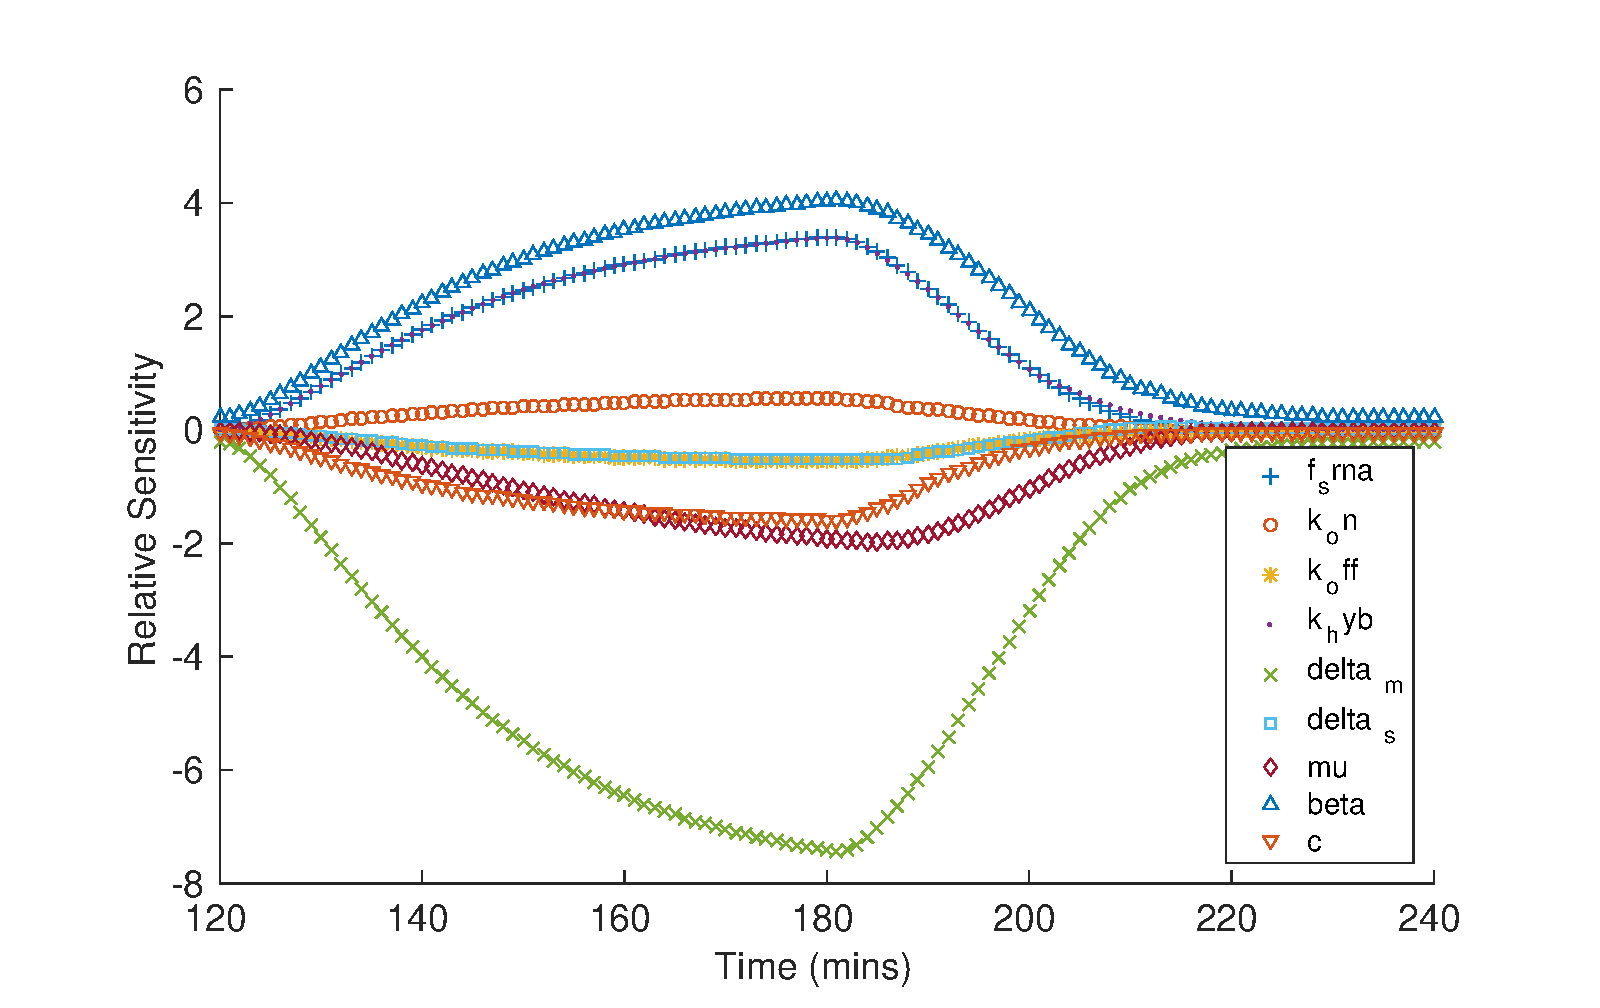
\includegraphics[scale = 0.23,clip = true, trim = 110 0 60 0]{Sensitivity_unscaled}
        \caption{Unscaled}
        \label{SensitivityMatrix_unscaled} 
    \end{subfigure}
    \begin{subfigure}[h]{0.49\textwidth}
    \centering
        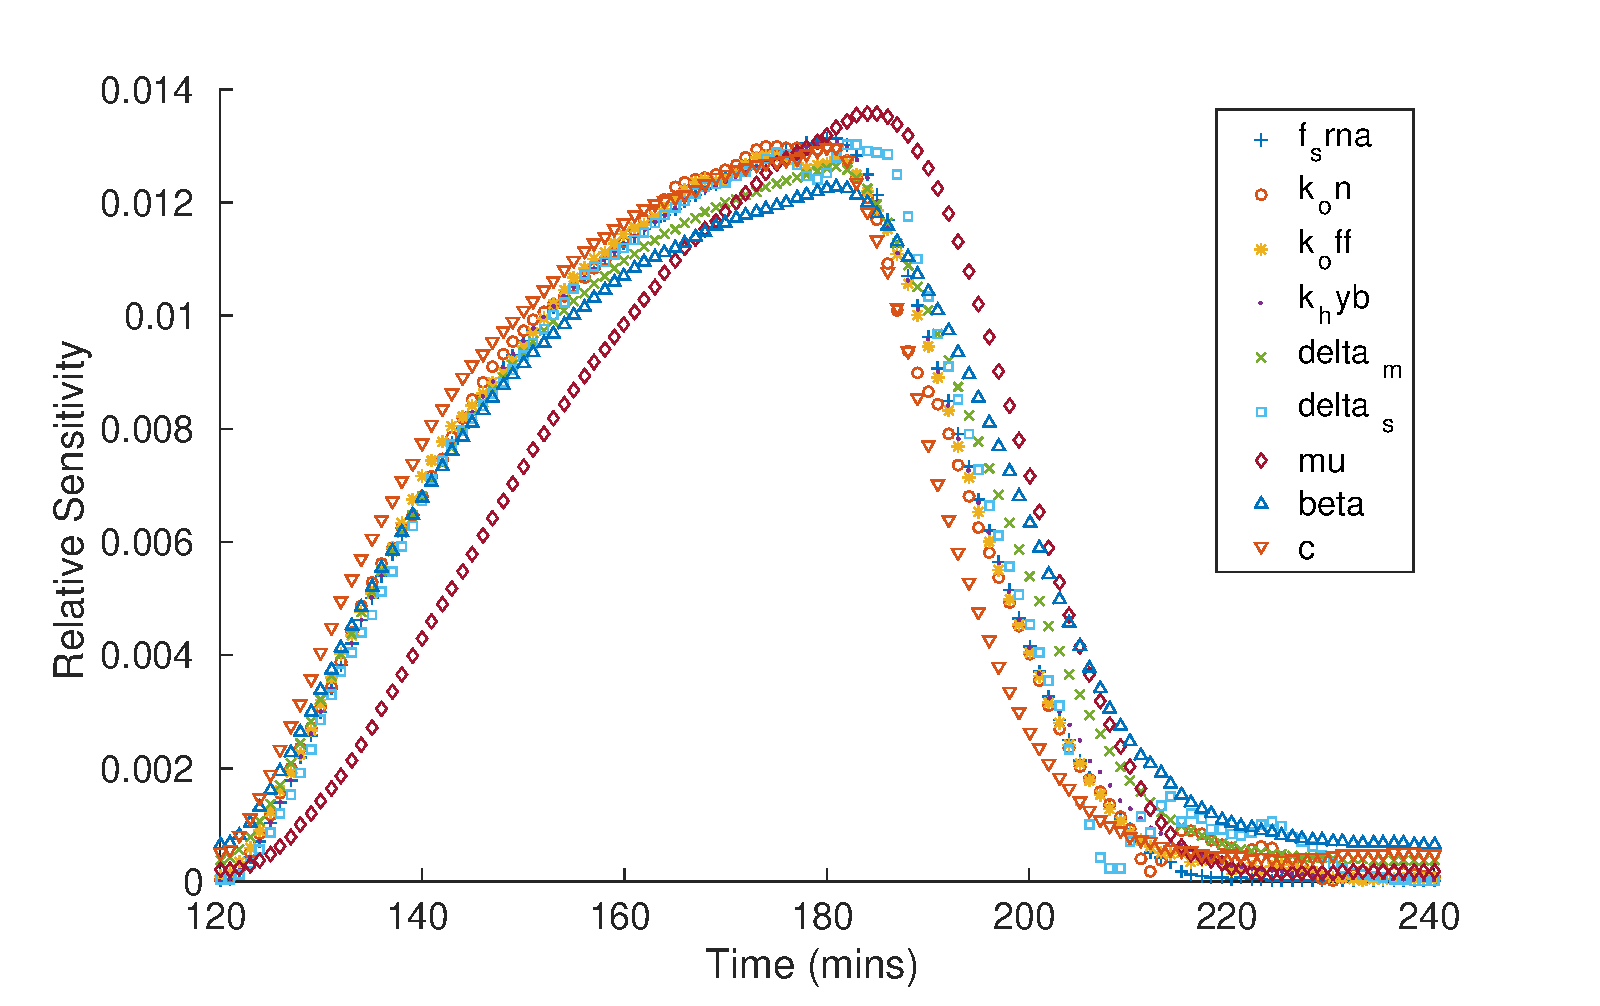
\includegraphics[scale = 0.23,clip = true, trim = 70 0 60 0]{Sensitivity_scaled}
        \caption{Scaled}
                \label{SensitivityMatrix_scaled} 
    \end{subfigure}
    \caption{Sensitivity coefficients $S_{ij}$ evaluated about a set of estimated parameters from the \textit{13\_9} dataset, for a single oscillation. \ref{SensitivityMatrix_unscaled} shows them unscaled, \ref{SensitivityMatrix_scaled} shows them scaled by the norm of each column of $S$.} 
\label{SensitivityMatrix}   
\end{figure}

We see that many of the parameters give sensitivity curves of similar shapes, and have near linear dependence - this implies that the effects of perturbing any one of these parameters all look similar in terms of model output, and are hard to distinguish between. This may help to explain why some of our initial parameter estimates are very loose, and why there are correlations between the estimated parameter sets - this result suggests there is a family of parameters all of which, in terms of the model output we have available, cannot be resolved. As such, we should view estimates of these parameters with extreme caution. Note that the sensitivity curve that looks least similar to the others in Fig. \ref{SensitivityMatrix_scaled} - $\mu$ - corresponds to a relatively tightly estimated value in Fig. \ref{InitialResults}.


 
\subsection{Differing timescales within the system}

Fig. \ref{model_output} shows model output for all state variables, using the parameter values giving the lowest error on the \textit{13\_9} dataset, and normalised to lie on the same scale. We see that $s,m,s:m$ and $c$ respond rapidly to the forcing function, flipping between the two fixed points defined by the step function forcing almost instantly. By contrast, there is delay in the response of $p$ and $g$, on a timescale comparable to the period of the forcing. This result suggests that, at least in some of the parameter sets initially estimated, the system may have two timescales in it - a fast timescale in which \eqref{eq:s} - \eqref{eq:c}, representing the hybridization of the sRNA and mRNA into a stable complex, equilibrate in response to external forcing, and a slower timescale, in \eqref{eq:p}, \eqref{eq:g}, in which measured fluorescence changes in response to the forcing.

\begin{figure}[h]	
    \centering
        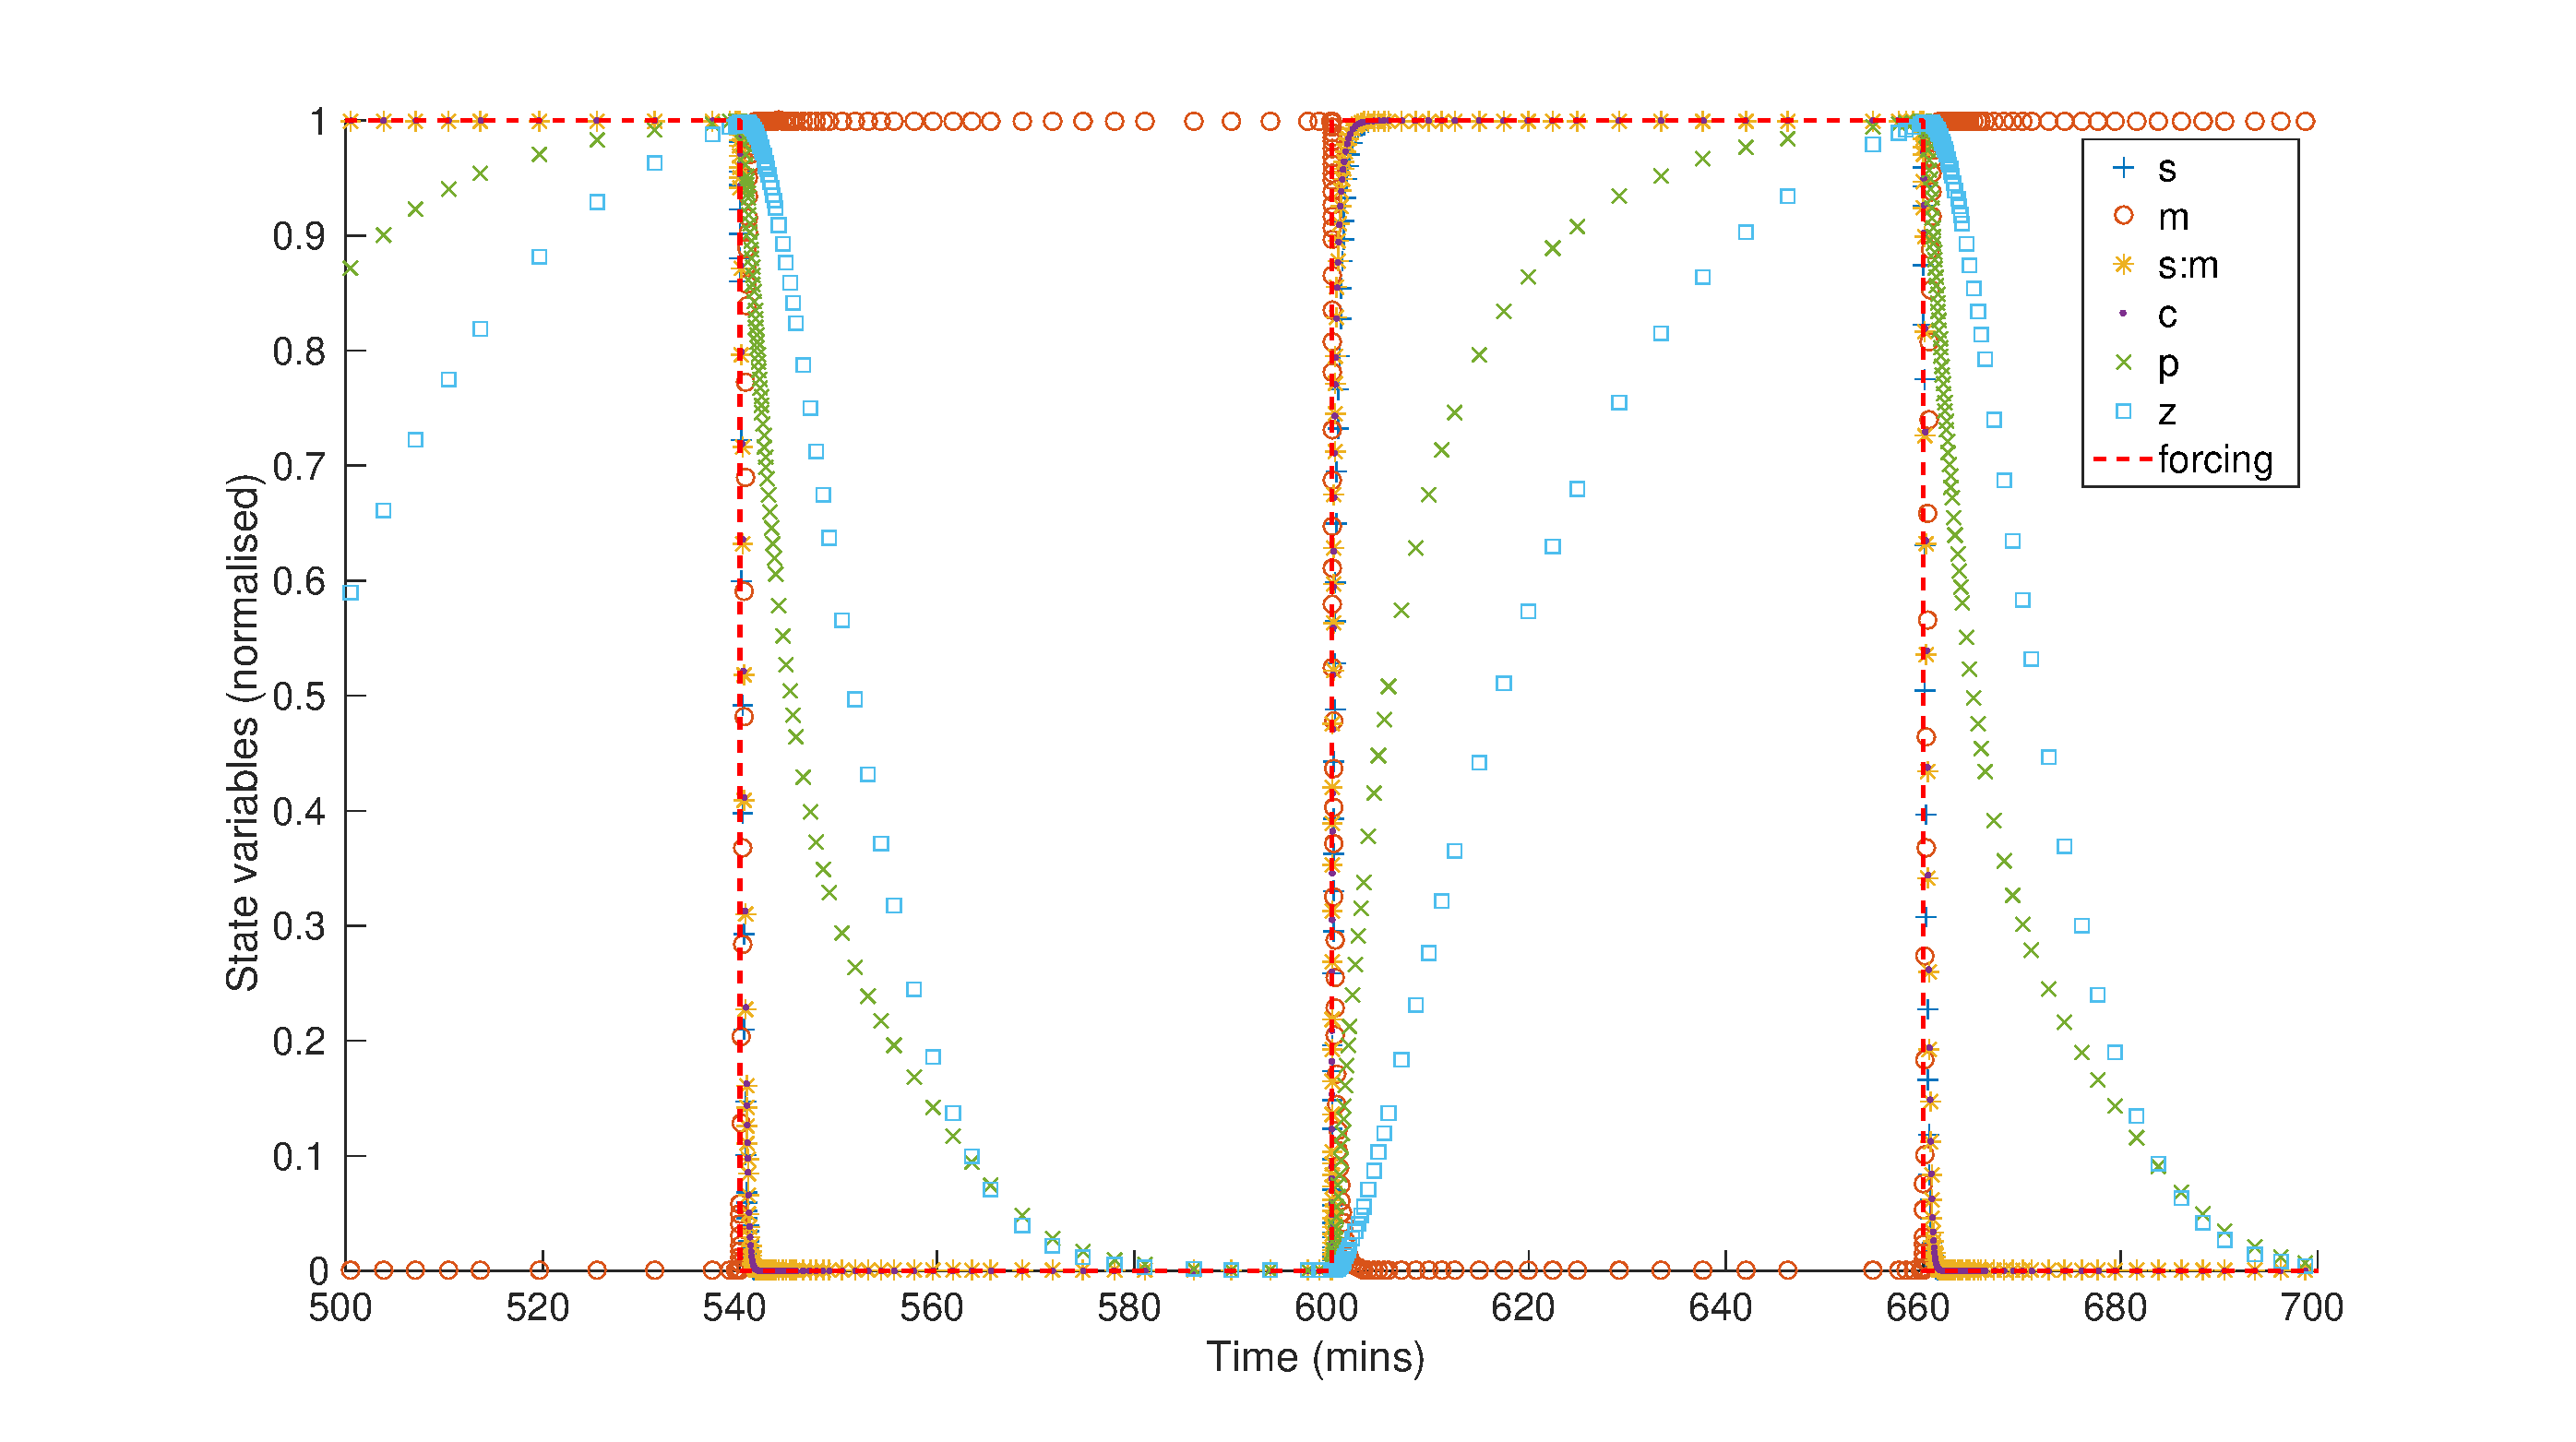
\includegraphics[scale = 0.26,clip = true, trim = 90 0 60 0]{model_output}
        \caption{Model output for all state variables over two oscillations, using the parameter values giving the lowest error on the \textit{13\_9} dataset, and normalised to lie on the same scale. Note $g$ is not explicitly shown, but is simply a rescaling of $z$ and as such would lie over it. }
        \label{model_output} 
\end{figure}

If this is the case, then it may be that our experimental data can only probe the system via the fixed point of \eqref{eq:s} - \eqref{eq:c} , and that the parameters contained within those equations can only work to set the particular fixed point values of $p$ and $g$ that the system tends toward. This would explain the similarity between the sensitivity curves of many parameters - if the parameters in \eqref{eq:s} - \eqref{eq:c} can only act to alter the model's fixed point, they would all alter the sensitivity curve in exactly the same way, since a small perturbation in one of these parameters would only act to perturb the location of the models fixed points. It would also suggest that all parameter sets giving the same value of the models fixed point will give similar model predictions - and there may be many, very different, parameter sets which all give the same fixed point. 

The fixed point values of $s,m, s:m$ and $c$ affect \eqref{eq:p}, \eqref{eq:g} through the $\beta m +f_{s}\beta c$ term in \eqref{eq:p}. Explicit forms for $m$ and $c$ are given in \eqref{eq:m_fixed}, \eqref{eq:c_fixed}. The fact that this term is  the only one in \eqref{eq:p}, \eqref{eq:g} to include $f_{s}$ and $\beta$ may also explain the similarity of the sensitivity curves for these parameters to those found in \eqref{eq:s} - \eqref{eq:c} (Fig. \ref{SensitivityMatrix_scaled}) - all that $p$ and $g$ see is this $\beta m +f_{s}\beta c$ flipping between its two fixed point values, so any parameters that only enter the system via this term will have indistinguishable roles.

Although we have seen that parameter sets with similar least squares error values can contain very different parameter values, this explanation implies that we would expect similar values of $\beta m +f_{s}\beta c$ across all the sets. Fig. \ref{fixedpoint_f} shows a scatterplot of $\beta m +f_{s}\beta c$  values against error function value, and demonstrates that, though individual parameter values can be spread across very large ranges, they are correlated in such a way as to give similar model fixed points. 

In Fig. \ref{fixedpoint_mu}, we also see a strong positive correlation between the fixed point values and the values of $\mu$ ($R = 0.9854$ for the visually tightly clustered data). Taken together with the relatively tightly constrained values of $\mu$ found in Fig. \ref{InitialResults}, these results suggest that in order to minimize error, the algorithm is effectively trying to vary $\beta m +f_{s}\beta c$ and $\mu$, and finding a `trench' of highly correlated values, which is shown in Fig. \ref{fixedpoint_mu}. 

These results further suggest that, while we are trying to minimise model error over our initial high dimensional space, we are effectively working in a lower dimensional space, in which one dimension is the value of the models $\beta m +f_{s}\beta c$ .


\begin{figure}[h]	
    \centering
        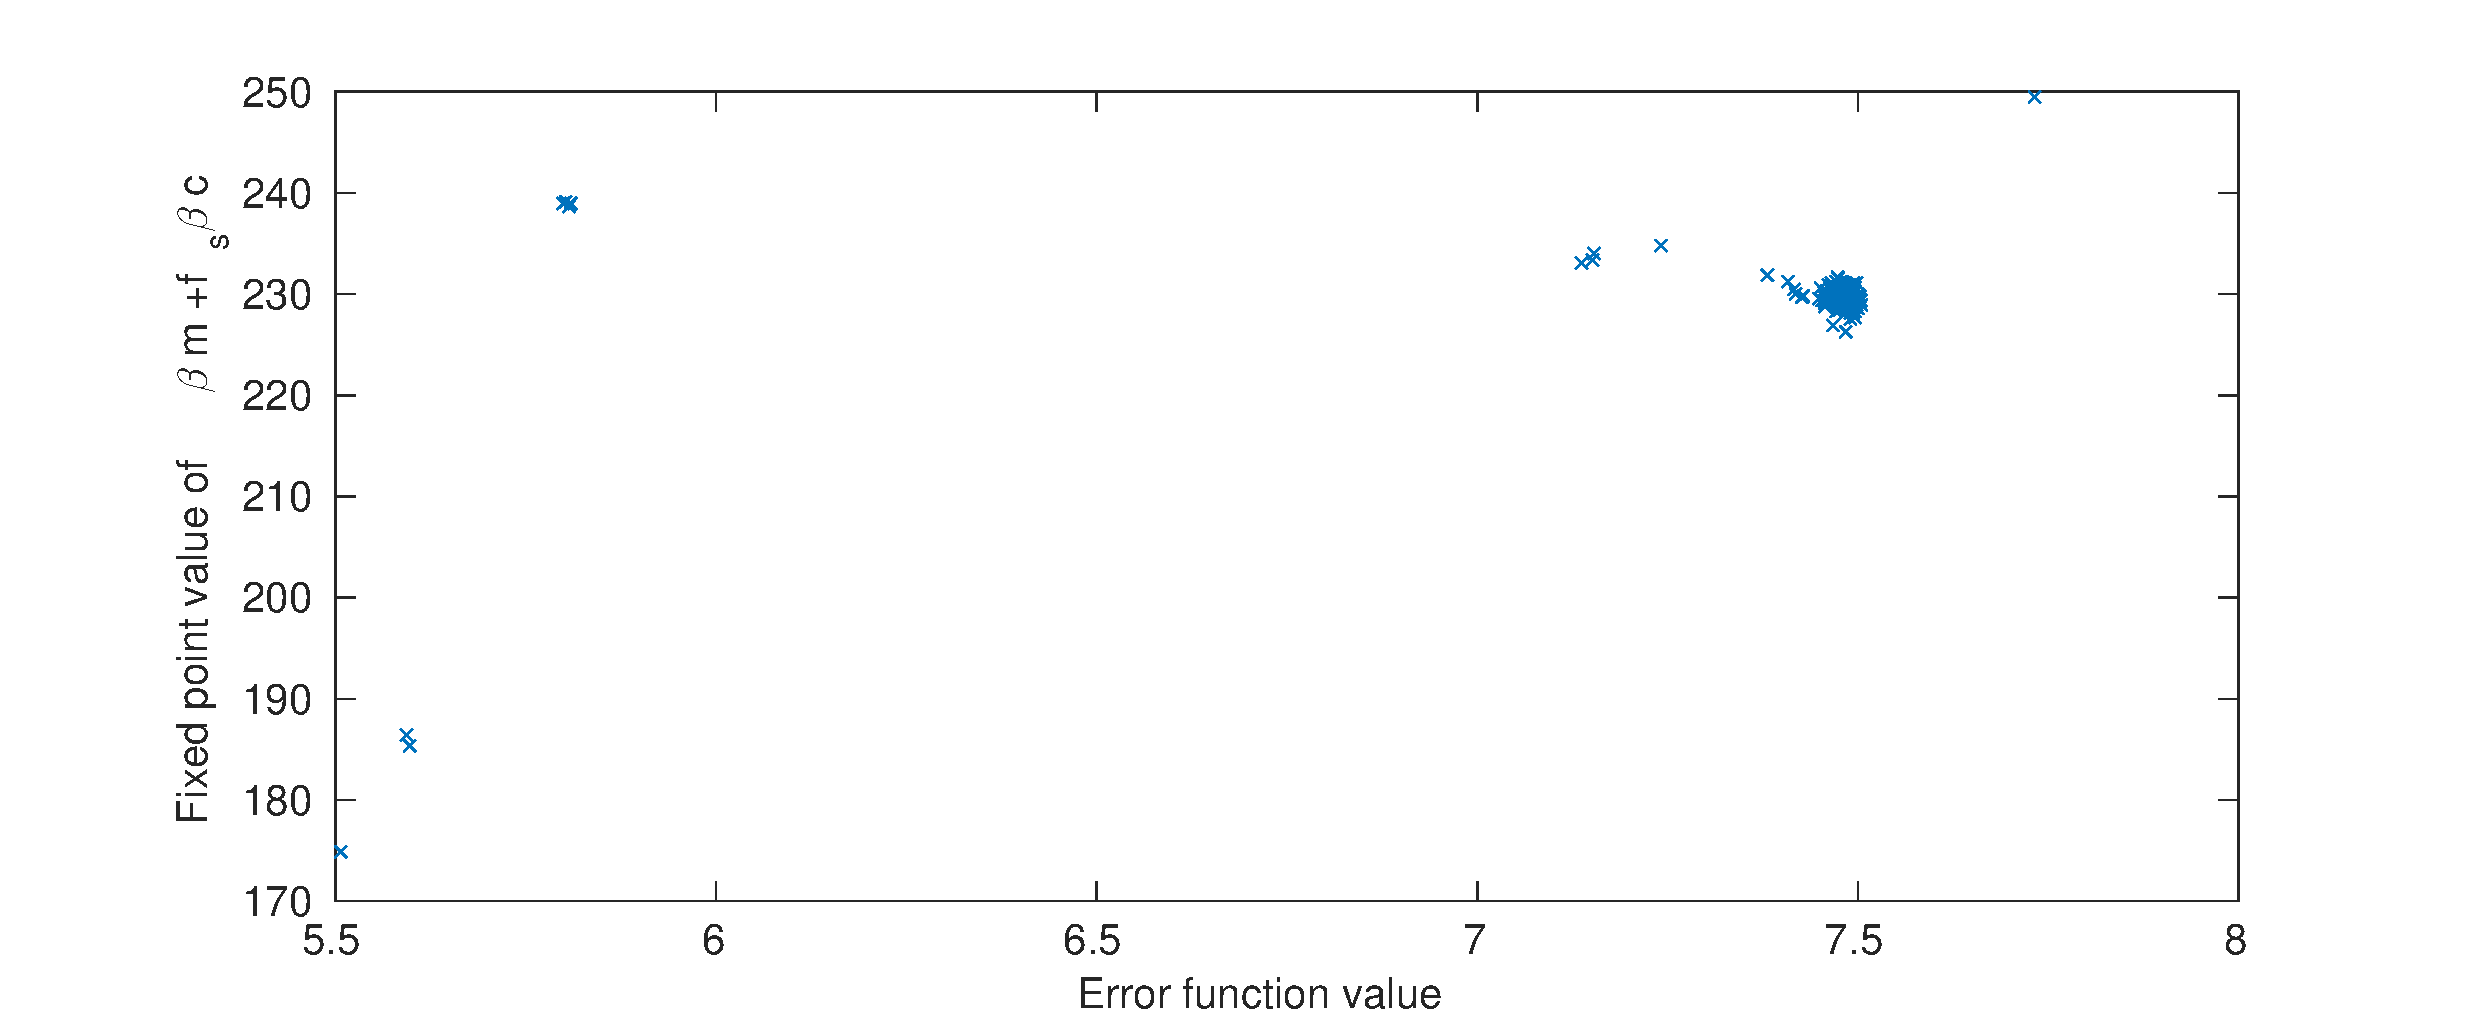
\includegraphics[scale = 0.25]{fixedpoint_f}
        \caption{A scatterplot of the fixed point value of $\beta m +f_{s}\beta c$, for a given parameter set, against the error value of that set. }
        \label{fixedpoint_f} 
\end{figure}

\begin{figure}[h]	
    \centering
        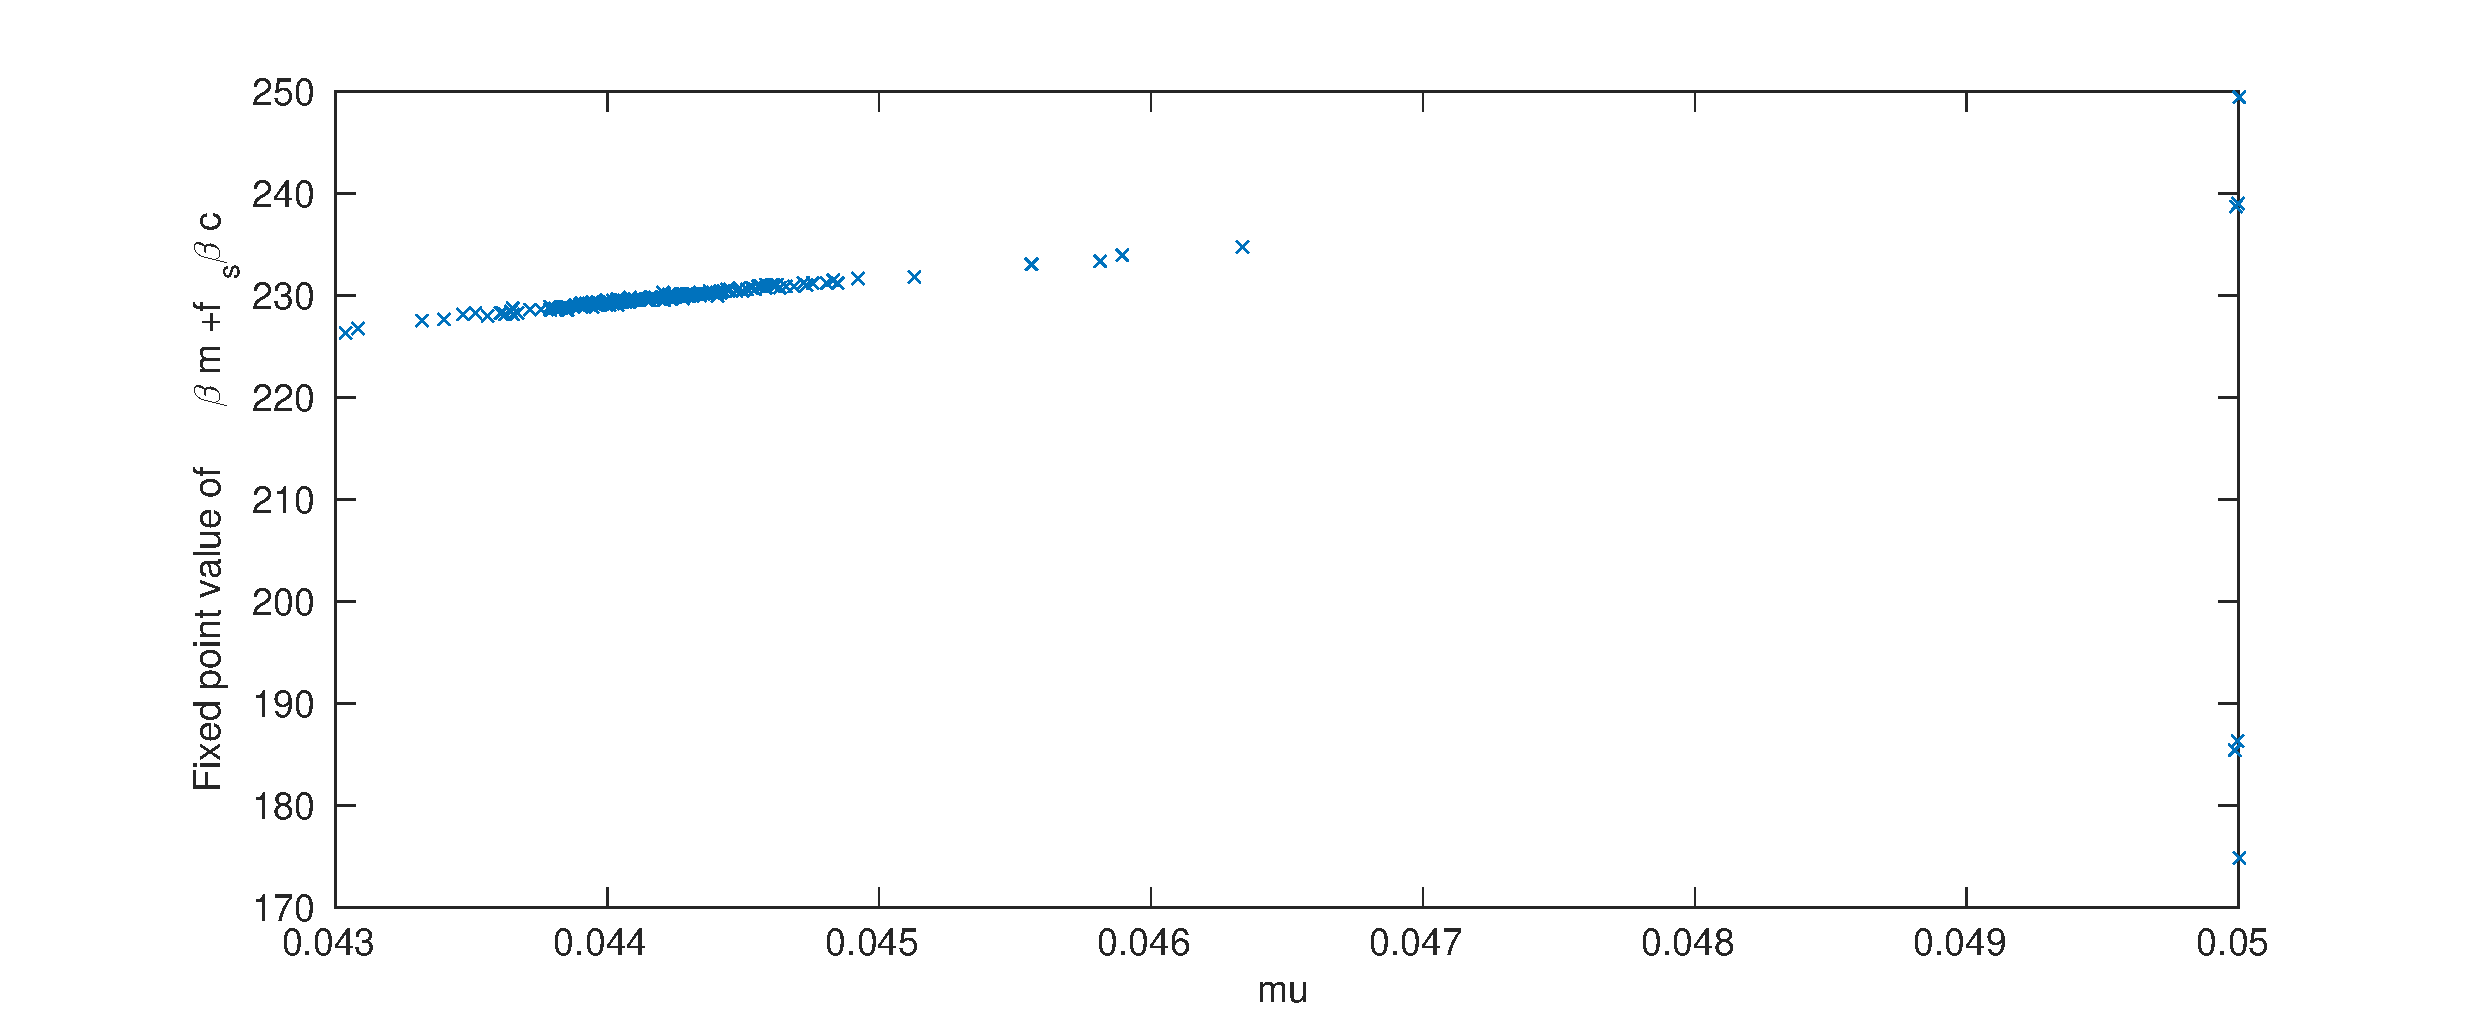
\includegraphics[scale = 0.25]{fixedpoint_mu}
        \caption{A scatterplot of the fixed point value of $\beta m +f_{s}\beta c$, for a given parameter set, against the value of $\mu$ in that set.}
        \label{fixedpoint_mu} 
\end{figure} 


 
 
\section{Conclusions and Further work}
\label{Conclusions and Further work}

In this report, we have presented a system of ODE's to model a recently proposed synthetic RNA regulatory circuit \cite{Rodrigo2012}. We have attempted to estimate the model's parameters using existing time series data, with a least squares minimisation approach, similar to that found in recent system biology literature \cite{Hu2015}. Where this approach has failed to give estimates, we have discussed in detail how the method has broken down.

 
The results in this paper suggest that, even though the model has a solid biological rationale, some parameters included in it may not be estimable. We have suggested practical reasons for this, namely that the effects of the parameters are highly correlated with one another, because the relevant quantity for determining a model prediction is not the full parameter set, but only the fixed point values of $\beta m +f_{s}\beta c$, and $\mu$. Thus the parameters in \eqref{eq:s} - \eqref{eq:c} only work to alter the fixed point value of $\beta m +f_{s}\beta c$, and so all have a qualitatively identical effects on model predictions. Effectively our algorithm is only working in a 2 dimensional space, varying $\beta m +f_{s}\beta c$ and $\mu$ to minimize error. This result suggests that using any additional step function data available may not help in determining the parameters - all of these step functions are applied at timescales over which the `fast' part of the model responds instantly, and so essentially tell us the same thing about the parameters contained in those equations. The different sets may give more information about $\mu$, which appears to work on a timescale comparable to the forcing.  

We note that it is possible that this separation of timescales is an artefact of the fitting, and not necessarily true of the system. We can only evaluate model predictions on the parameter sets the algorithm returns us, and it seems the case that the parameter sets found by the algorithm have this feature. Hypothetically, there may exist parameter sets where all state variables vary on a similar timescale - all we can say is that, in the search region specified, the algorithm has not found any which give a low error. 

This point raises another issue - the arbitrary nature of the initial bounding box. Without good biological constraints on most parameter values, they have been bounded loosely and not necessarily sensibly. Rate constants can vary by many orders of magnitude, and it may be possible that the true optimum lies entirely outside the bounding box specified. Equally,  when our fitness function has turned out to be very flat in some directions, or multimodal, good biologically motivated parameter bounds may be needed to ensure our minimisation algorithm does not wander outside realistic parameter space - the algorithm may present several equally good regions of parameter space, and improved bounds will help us choose between them. We also note that while some parameters may be hard to get any realistic bounds on, values for others - $\mu, \Theta$ for example - may already be available.

 The model may also have general structural issues. \cite{Mclean2012, Grewal1976} give general tests which can be applied to a system of ODE's to determine if all parameters are, in principle, estimable. We note that our system has few enough parameters to make these tests feasible.
 
 Thus, further work may consist of tightening the bounds on parameter values, carrying out a structural analysis, and possibly simplifying the model. A much simpler phenomenological model, consisting of  just \eqref{eq:p} and \eqref{eq:g}, may explain existing data perfectly well without the need for inestimable parameters. Experimentally, one option  may be to use different forcing functions. The effect of this on parameter estimability might be anticipated by running a sensitivity analysis using this new forcing, to see if the form of Fig. \ref{SensitivityMatrix} (which shows model predictions for all states) changes. Another option, though perhaps experimentally infeasible, would be to directly observe other components of the state vector - $s$, $m$, $s:m$ and $c$. This would improve parameter estimates by giving direct observations of the effects of parameters contained in \eqref{eq:s} - \eqref{eq:c}.

Some earlier fitting work has been done on this dataset via a similar method to the one used above. Our results suggest that those estimates should be viewed with caution - the estimates will not be unique, and the values of some parameters (those in \eqref{eq:s} - \eqref{eq:c}) may be very far off any values which are eventually found.

These results also suggest general problems with our methodology - using a least squares minimisation approach. The first problem is local minima. Using the CMA-ES will give better results than a local minimisation algorithm, but you can never be sure you have found a global optimum - for example, \cite{Algorithms2003} compares several algorithms and finds, in the problem set, none locate the true global optimum. A related problem is that of working with single points rather than distributions on parameter space. The CMA-ES will only ever find a single optimum, but in the case where the error landscape is very flat -  for example a flat basin pocketed by many local minima - the exact minimum it finds paints a misleading picture, because it gives no idea of the uncertainty in the answer given. To surmount this problem, we may rerun the algorithm many times, from many starting locations, and interpret the resulting spread of parameter values found as an uncertainty \cite{Hu2015}, as we have done in this report. However this methodology is rather ad hoc.

A more systematic approach might be to use Markov Chain Monte Carlo (MCMC) for the parameter estimation \cite{Jitjareonchai2006,Andrieu2003}. This method would explicitly provide us with marginal distributions of parameters, giving a more complete and systematic picture of the best parameter sets and their uncertainties than we currently have - we would still be able to pick out a Maximum Likelihood point estimator, as we do now, but rather than getting an ad hoc picture of the uncertainty in the parameters by repeatedly running the minimisation algorithm, the marginals would give us this information directly.

\todo[inline]{write section on GP's}.

% references section
\begin{footnotesize}
\bibliographystyle{./IEEE_bibtex_class/IEEEtran}
\bibliography{./IEEE_bibtex_class/IEEEabrv,library}
\end{footnotesize}
\clearpage
\onecolumn

\appendices
\renewcommand\thefigure{\thesection.\arabic{figure}}  


\section{Initial Experimental Data}
\label{Initial Experimental Data}
\setcounter{figure}{0}    

\begin{figure}[h]
\centering
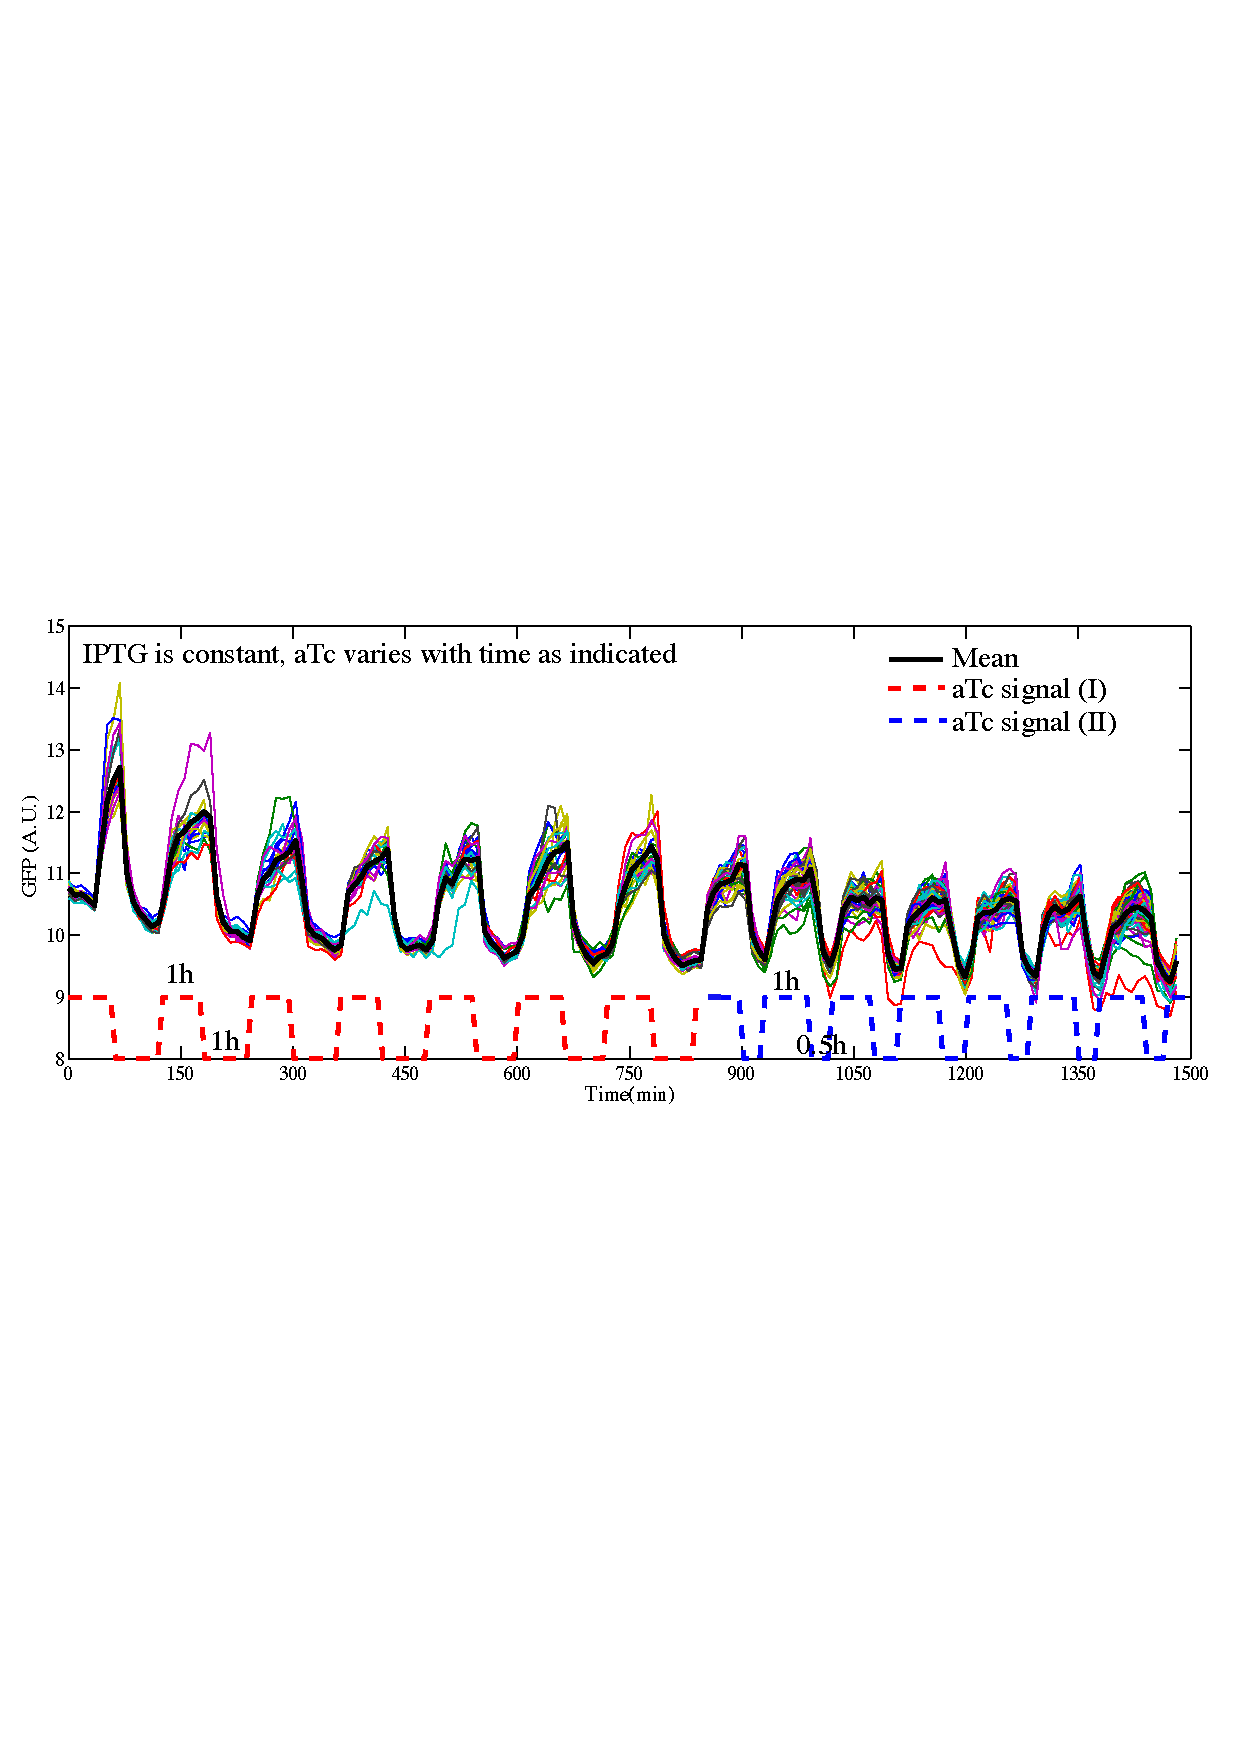
\includegraphics[trim = 0 310 0 300 , scale = 0.7, clip = true]{13_9}
\caption{The \textit{13\_9} dataset, with aTc forcing shown. IPTG concentration is constant at a level which saturates the cell's response. Note the forcing curve's height is schematic - aTc concentation is switched between off, and a level which saturates the cell's response}
\label{}
\end{figure}

%trim=l b r t
\begin{figure}[h]
\centering
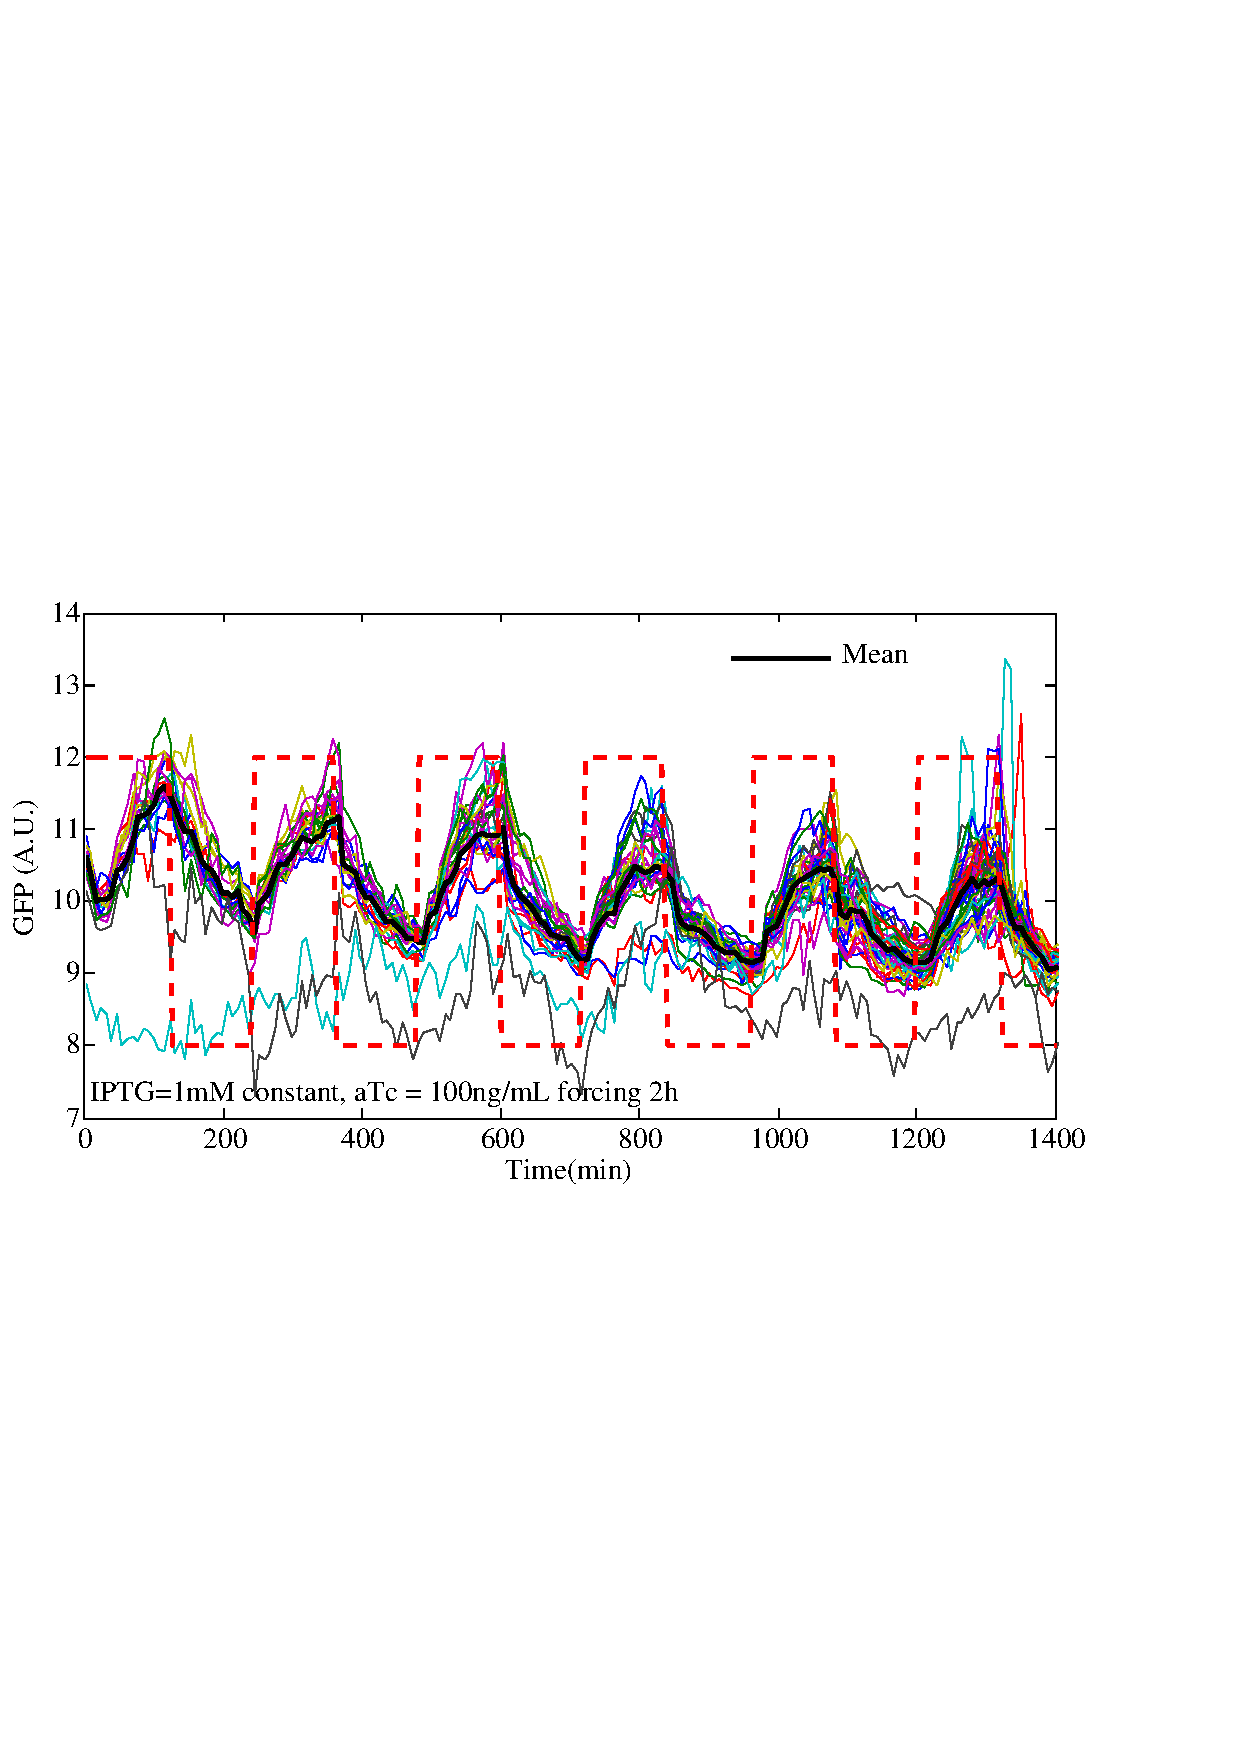
\includegraphics[trim = 0 270 0 250 , scale = 0.7, clip = true]{14_7}
\caption{The \textit{14\_7} dataset, with aTc forcing shown. IPTG concentration is constant at a level which saturates the cell's response. Note the forcing curve's height is schematic - aTc concentation is switched between off, and a level which saturates the cell's response}
\label{}
\end{figure}


%\begin{figure}[h]
%\centering
%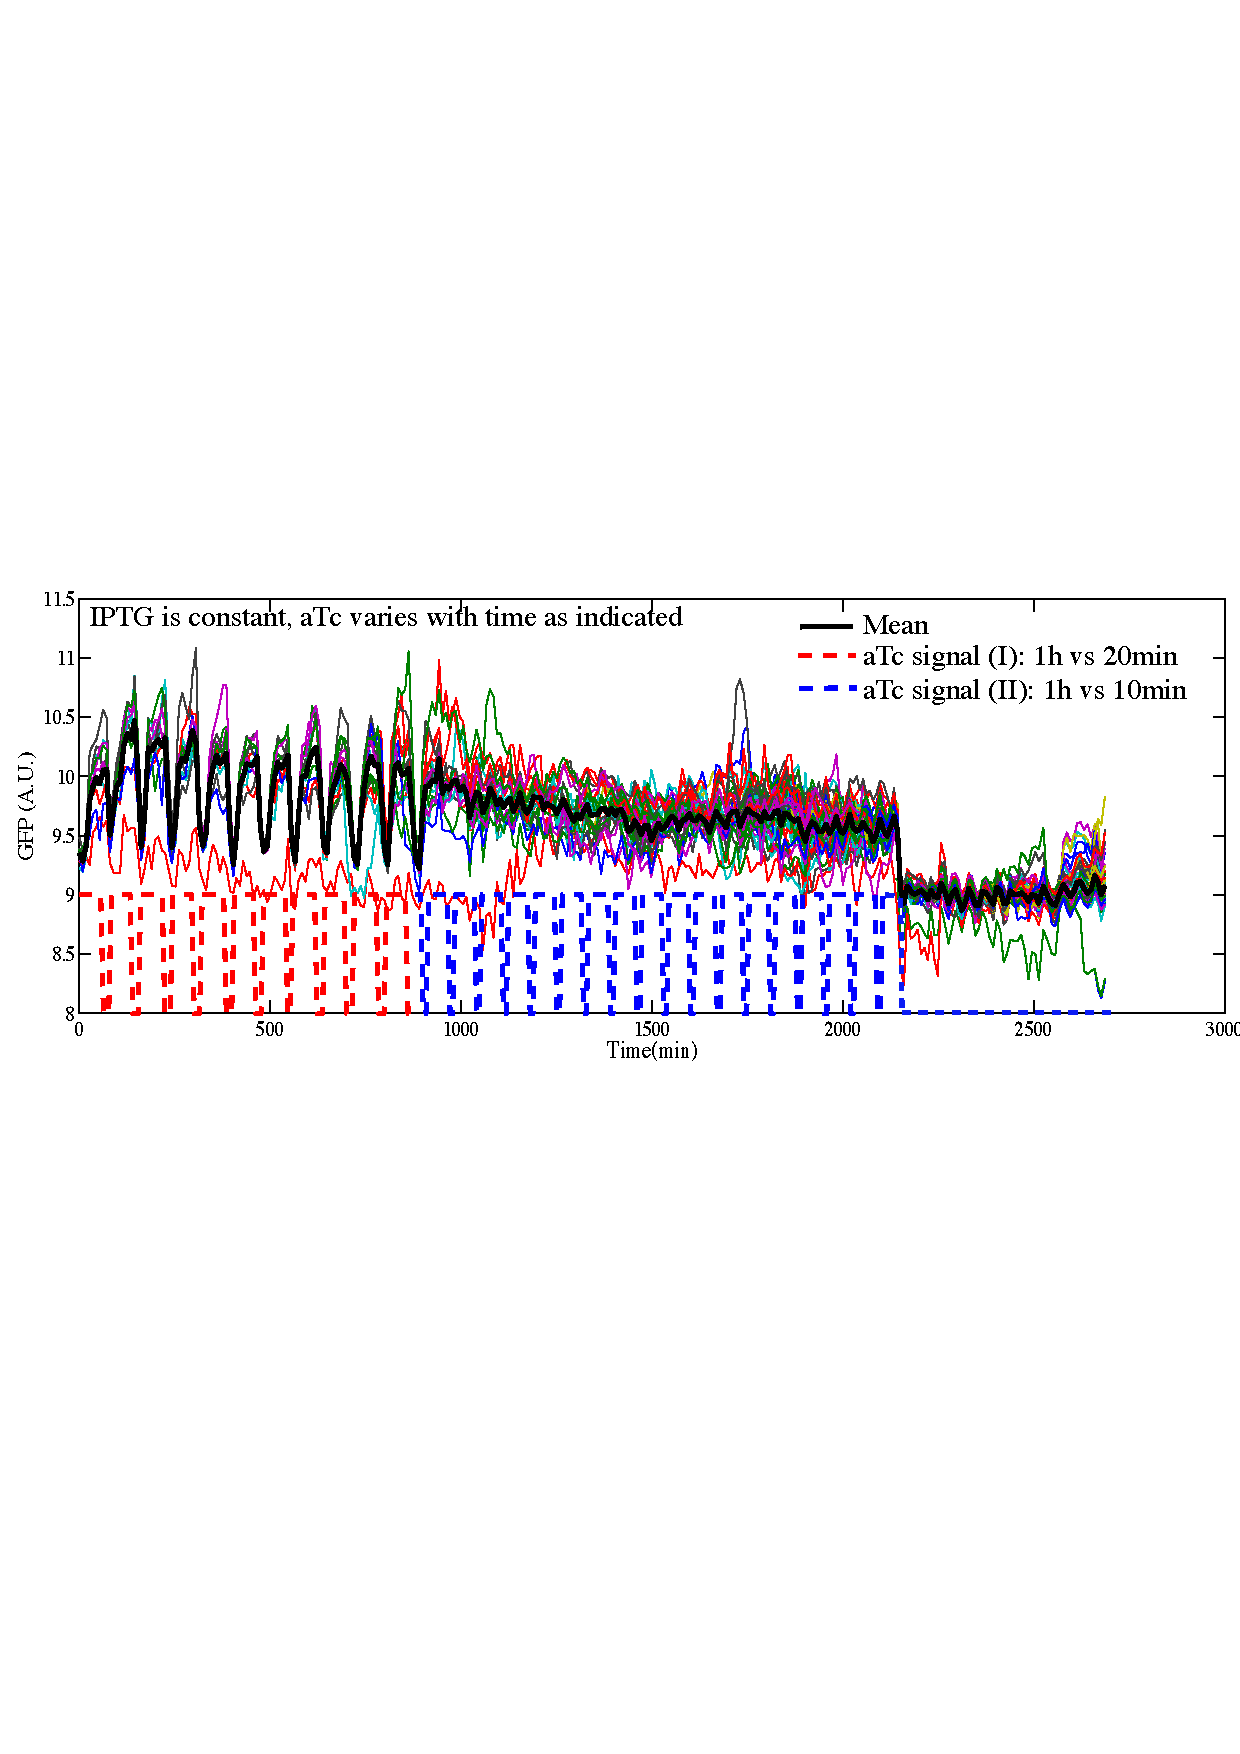
\includegraphics[trim = 0 330 0 270 , scale = 0.5, clip = true]{14_9}
%\caption{The \textit{14\_9} dataset, with aTc forcing shown. IPTG concentration is constant at a level which saturates the cell's response. Note the forcing %curve's height is schematic - aTc concentation is switched between off, and a level which saturates the cell's response}
%\label{}
%\end{figure}

\clearpage

\section{Parameter literature review}
\label{Parameter literature review}
\setcounter{figure}{0}    

\begin{table}[h!]
\renewcommand{\arraystretch}{1.3}
\caption{Literature references, or initial rough bounds, on parameter values, with those to be estimated shown in bold}
\centering
\begin{tabular}{| l | l | p{0.3\linewidth} | p{0.1\linewidth} | p{0.1\linewidth} |}
\hline \textbf{Parameter} &  \textbf{Value} & \textbf{Definition} & \textbf{Reference} & \textbf{Initial Bounds}  \\
\hline \hline N & 300 & Number of copies of promoter existing on plasmid DNA & Experimentally set & \\
\hline $z_{0}$ &   9 AFU & Baseline experimental fluorescence & Experimentally determined &  \\
\hline $\alpha_{L}$ & 11 nM/min & Maximal transcription rate of $P_\mathrm{LlacO-1}$ promoter & \cite{Lutz1997} &\\
\hline $\alpha_{T}$  & 11 nM/min  & Maximal transcription rate of $P_{\mathrm{LtetO-1}}$ promoter  & \cite{Lutz1997}& \\
\hline $f_{L}$ & 620 & Unitless ratio between repressed and unrepressed $P_\mathrm{LlacO-1}$ transcription rate  & \cite{Lutz1997}  &  \\ 
\hline $f_{T}$ & 2535 & Unitless ratio between repressed and unrepressed $P_{\mathrm{LtetO-1}}$ transcription rate   & \cite{Lutz1997} &\\
\hline $\delta_{g}$  & 0.0005 /min  & GFP degradation rate & \cite{Andersen1998} &\\
\hline $\gamma$ &  0.132 /min & GFP maturation rate & \cite{Iizuka2011} & \\
\hline $v_{z}$ & 100 nM/min & degradation constant of clpx & \cite{Hersch2004} &\\
\hline $K_{z}$   &   75 nM/min & Dissociation constant of clpx & \cite{Hersch2004} &\\
\hline $\boldsymbol{\Theta}$  &   nM/AFU & Ratio between GFP concentration and observed fluoresence & & 300 - 1000  \\
\hline $\boldsymbol{\mu}$ &  /min & Dilution rate & & 0.001-0.05\\
\hline $\boldsymbol{\delta_{m}}$ &  /min & mRNA degredation rate & & 1 - $10^5$ \\
\hline $\boldsymbol{\delta_{s}}$ &  /min & sRNA degredation rate & & 1 - $10^3$ \\
\hline $\delta_{sm}$ &  /min & Unstable sRNA:mRNA degradation rate & &  Set to $\delta_m$\\
\hline $\delta_{c}$ &  /min & Stable sRNA:mRNA degradation rate & & Set to $\delta_m$ \\
\hline $\boldsymbol{k_{on}}$ &   /min & sRNA:mRNA binding rate & & 100 - $10^7$\\
\hline $\boldsymbol{k_{off}}$ &  /min & sRNA:mRNA unbinding rate & & 1 -$10^8$\\
\hline $\boldsymbol{k_{hyb}}$ &  /min & sRNA:mRNA hybridization rate & & 1 - $10^4$ \\
\hline $\boldsymbol{\beta}$ &   /min & Baseline translation rate of repressed mRNA & & 0.0001 - 10\\
\hline $\boldsymbol{f_{s}}$ & & Ratio of repressed mRNA to unrepressed complex translation rate. & & 0.1 - $10^4$\\
\hline
\end{tabular}
\end{table}

\clearpage

\section{Histogram of Initial Fit Error values}
\label{Initial fit Error}
\setcounter{figure}{0}    

\begin{figure}[H]
    \begin{subfigure}[c]{\textwidth}
    \centering
        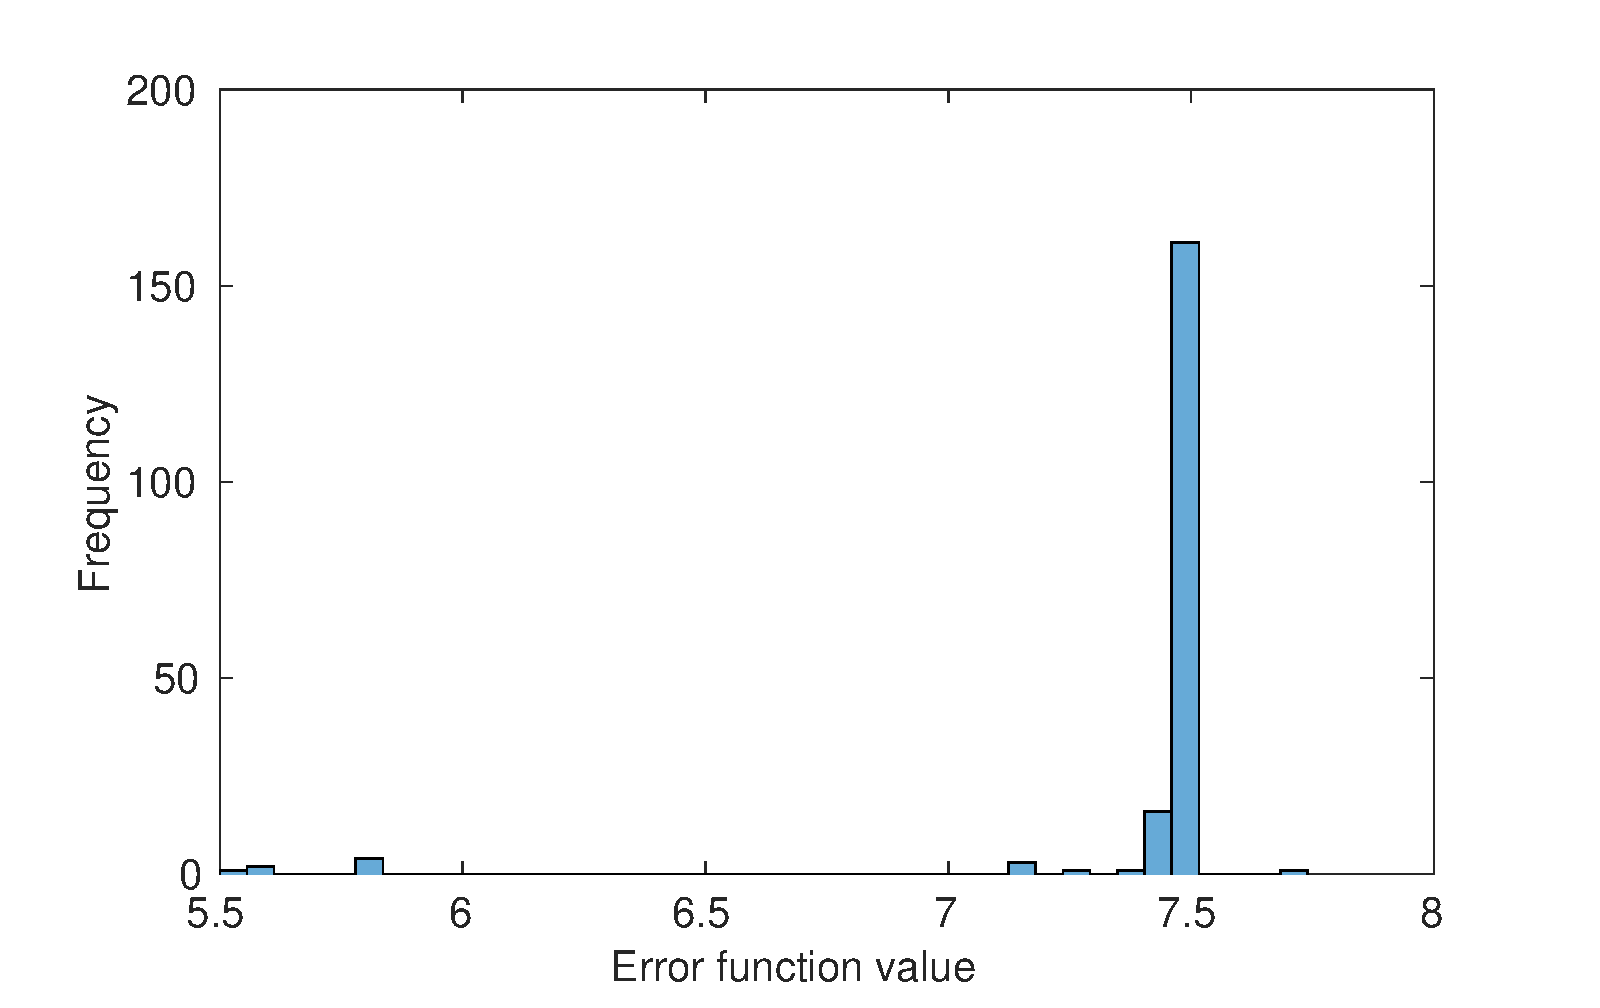
\includegraphics[scale = 0.5]{13_9_f_hist}
        \caption{Error values found from 200 initial parameter estimates, \textit{13\_9 dataset}.}
    \end{subfigure}
    
    \begin{subfigure}[c]{\textwidth}
    \centering
        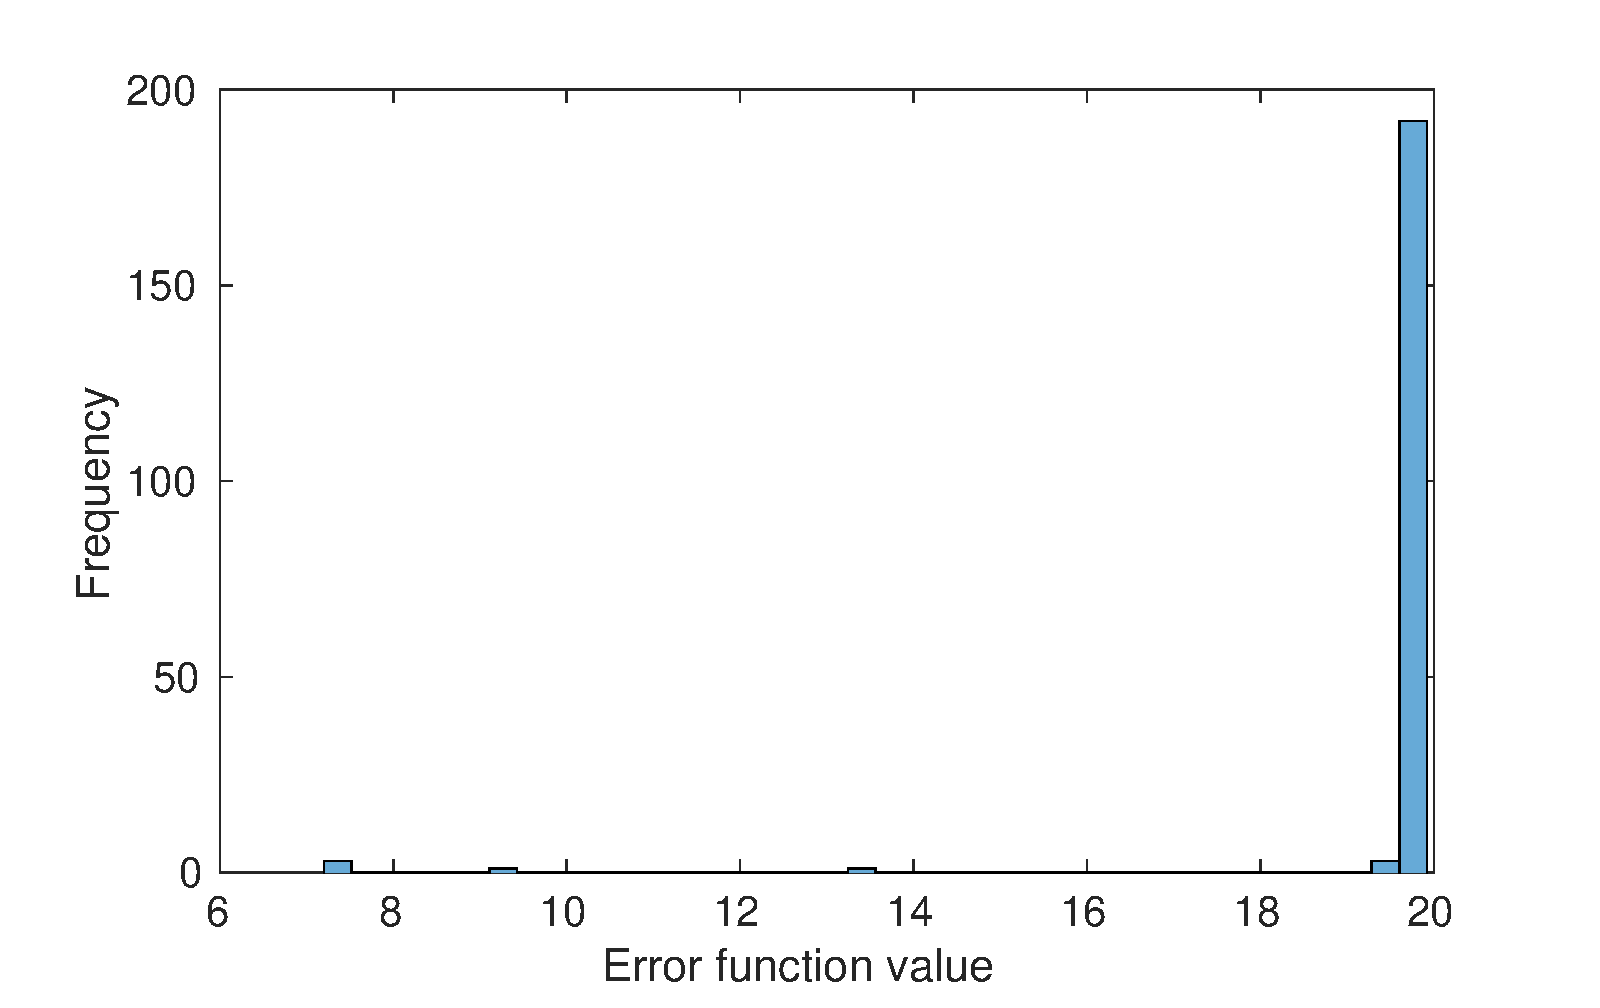
\includegraphics[scale = 0.5]{14_7_f_hist}
        \caption{Error values found from 200 initial parameter estimates, \textit{14\_7 dataset}}
    \end{subfigure}
    \caption{}
\label{hist_f}
\end{figure} 

\section{Initial parameter Estimates, both datasets}
\label{Bothdatasetfitting}
\setcounter{figure}{0} 

\begin{figure}[H]
    \begin{subfigure}[c]{\textwidth}
    \centering
        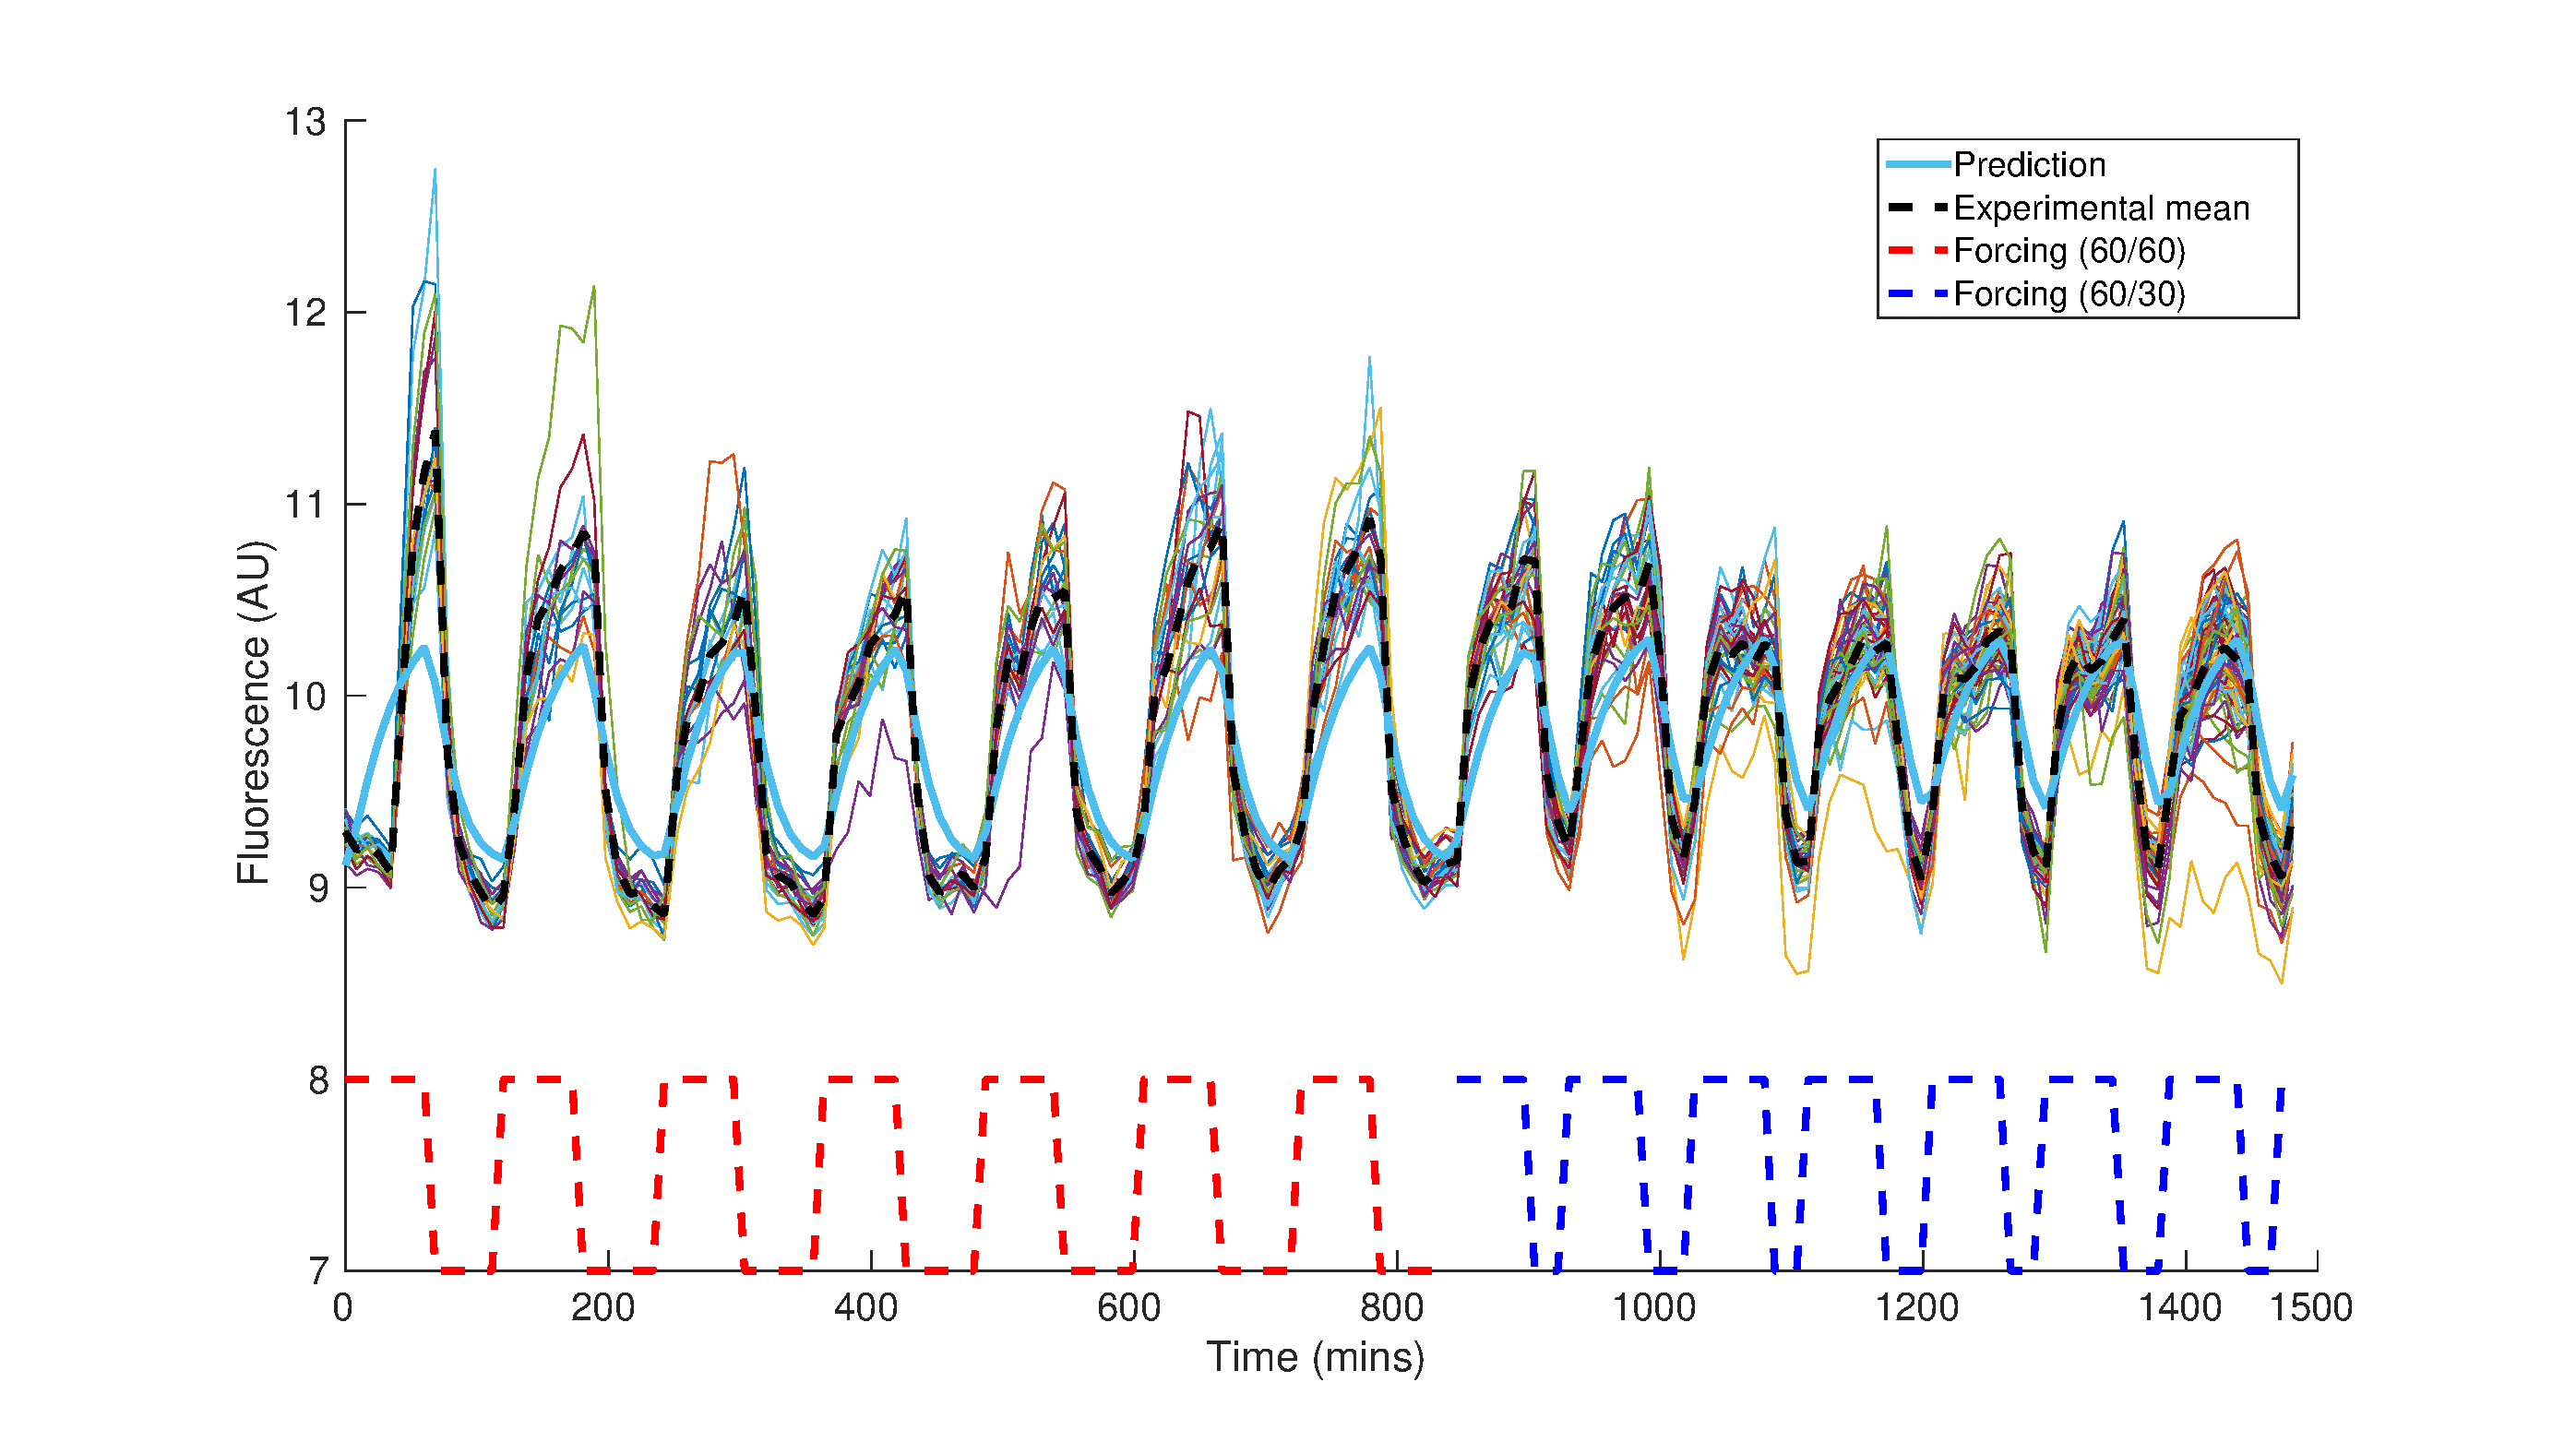
\includegraphics[scale = 0.3]{13_9_14_7_with_13_9_bestplot}
        \caption{Model prediction from parameter set which gives lowest error when trained on the combination of both datasets, plotted against the  \textit{13\_9} dataset. }
    \end{subfigure}
    
    \begin{subfigure}[c]{\textwidth}
    \centering
        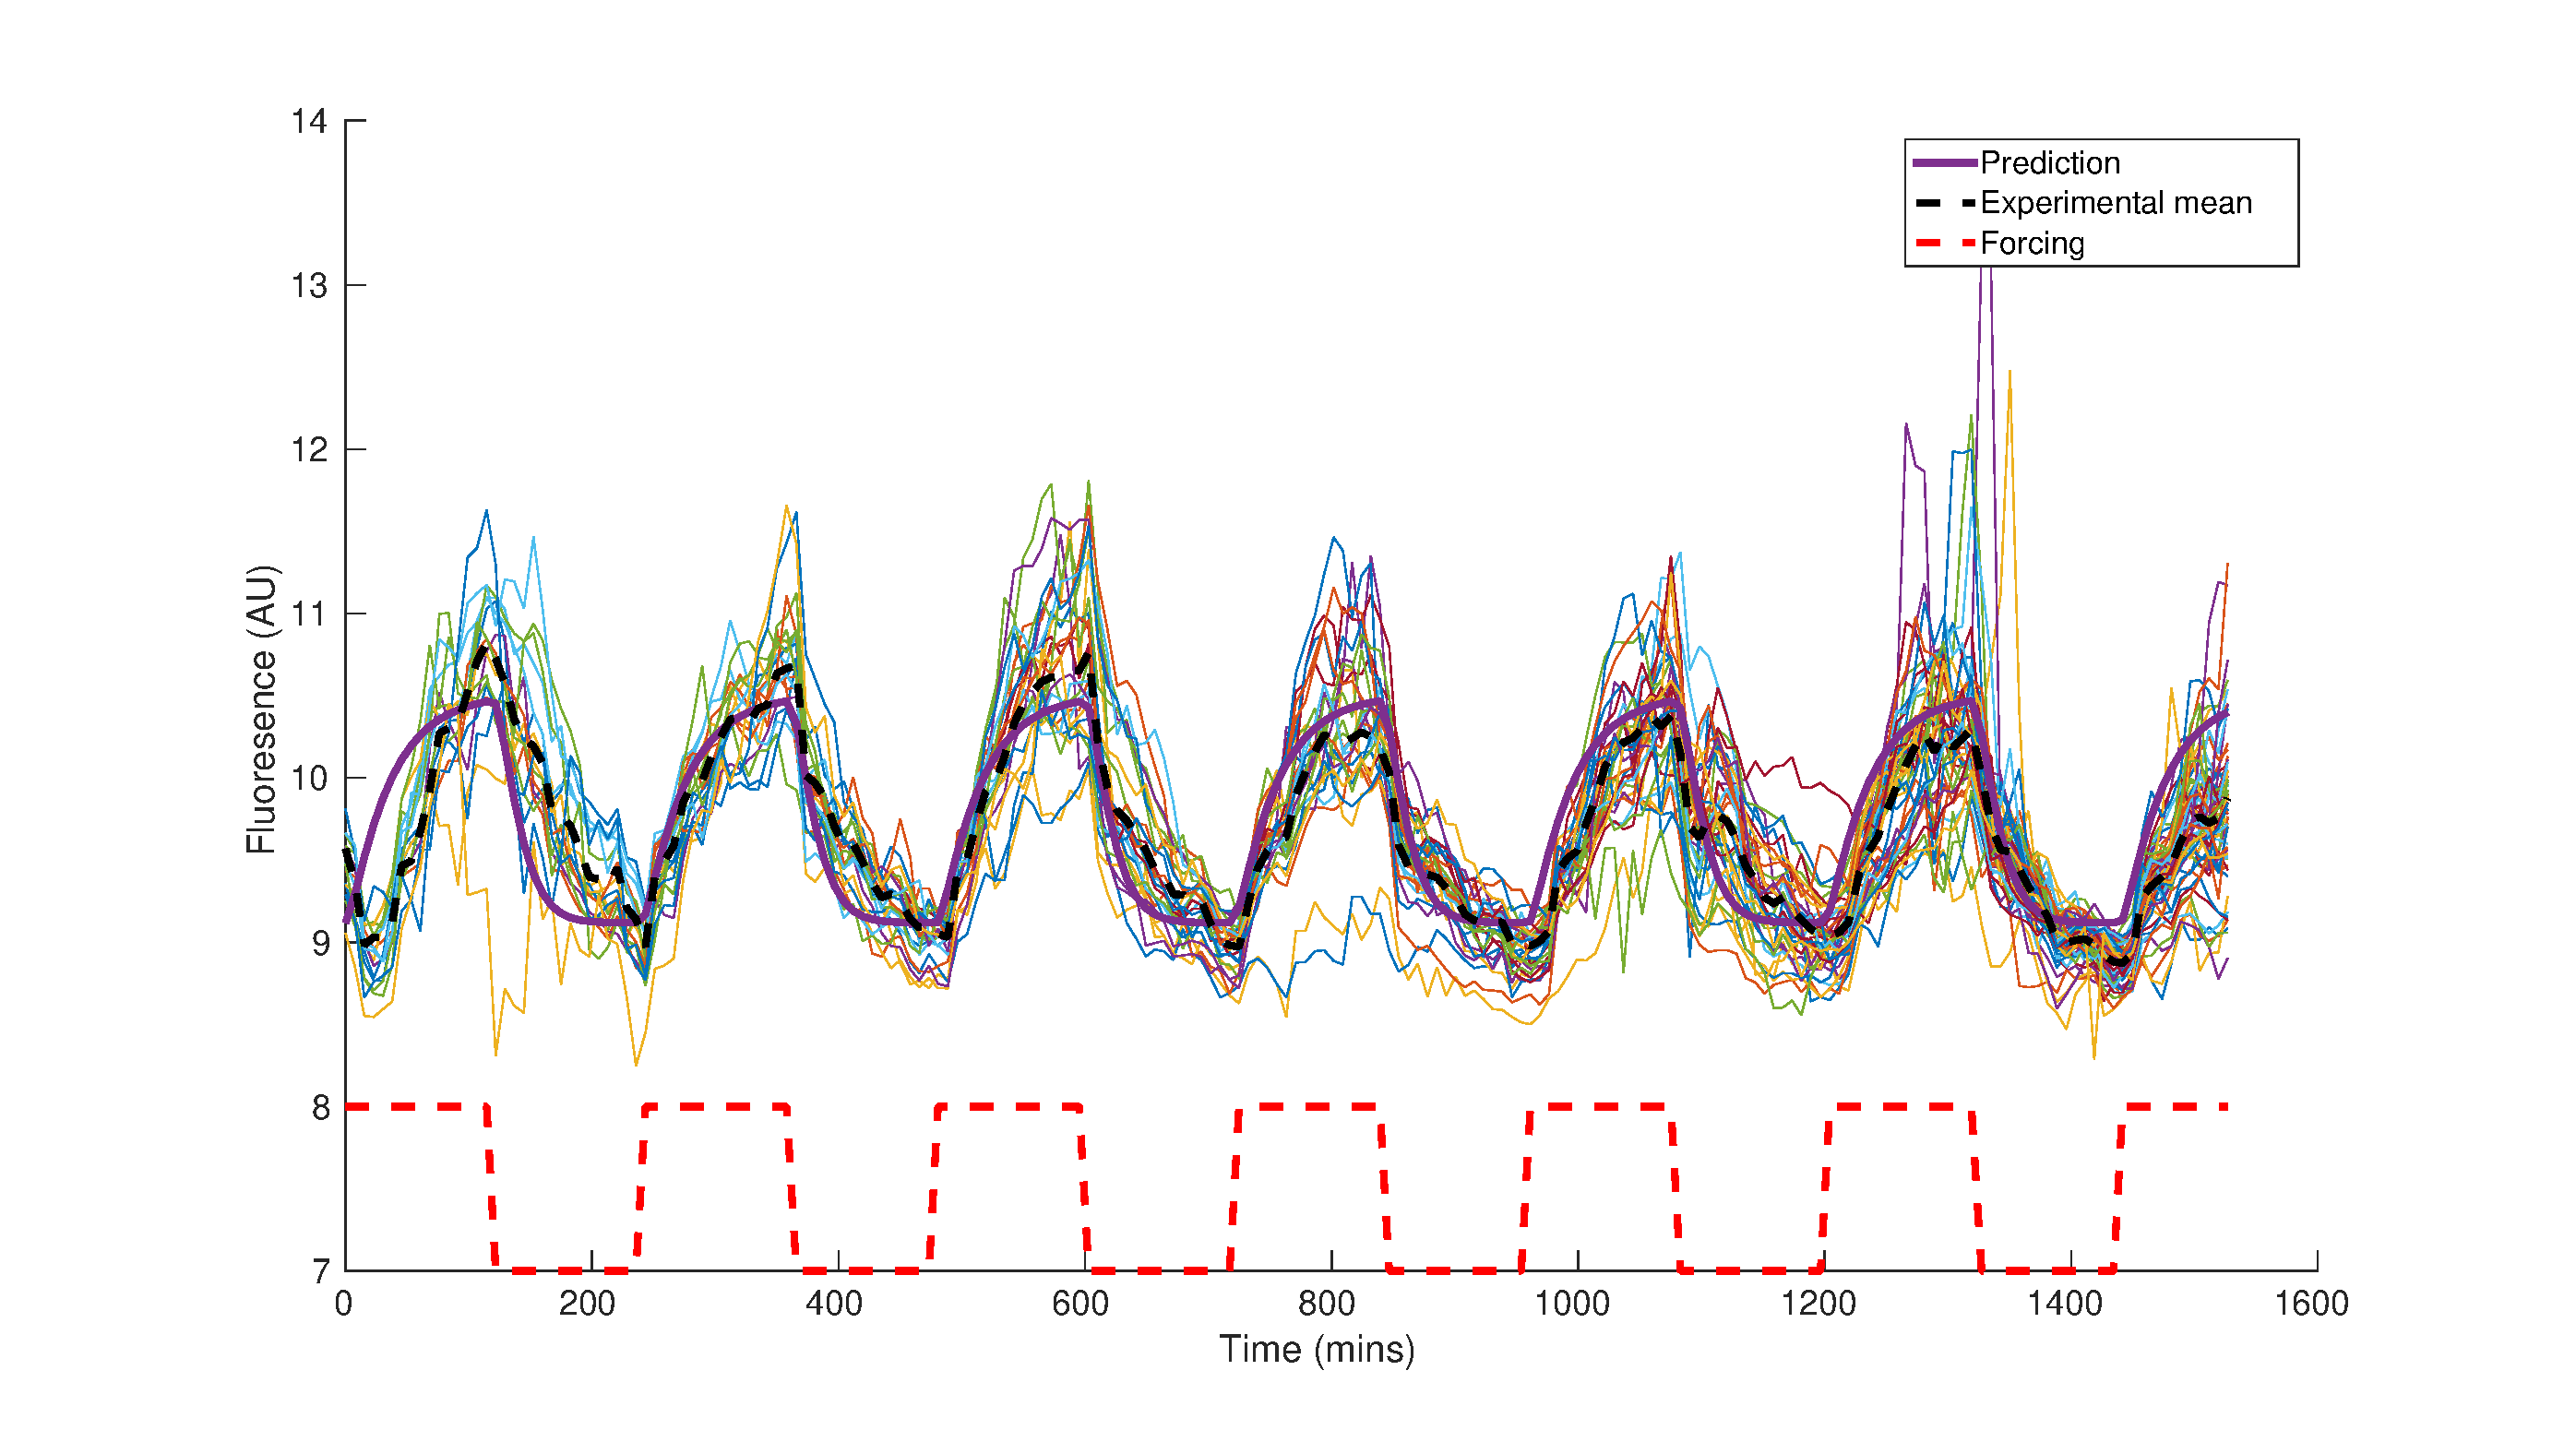
\includegraphics[scale = 0.3]{13_9_14_7_with_14_7_bestplot}
        \caption{Model prediction from parameter set which gives lowest error when trained on the combination of both datasets, plotted against the  \textit{14\_7} dataset.}
    \end{subfigure}
    \caption{}
\label{hist_f}
\end{figure}

\begin{figure}[H]
   \centering
        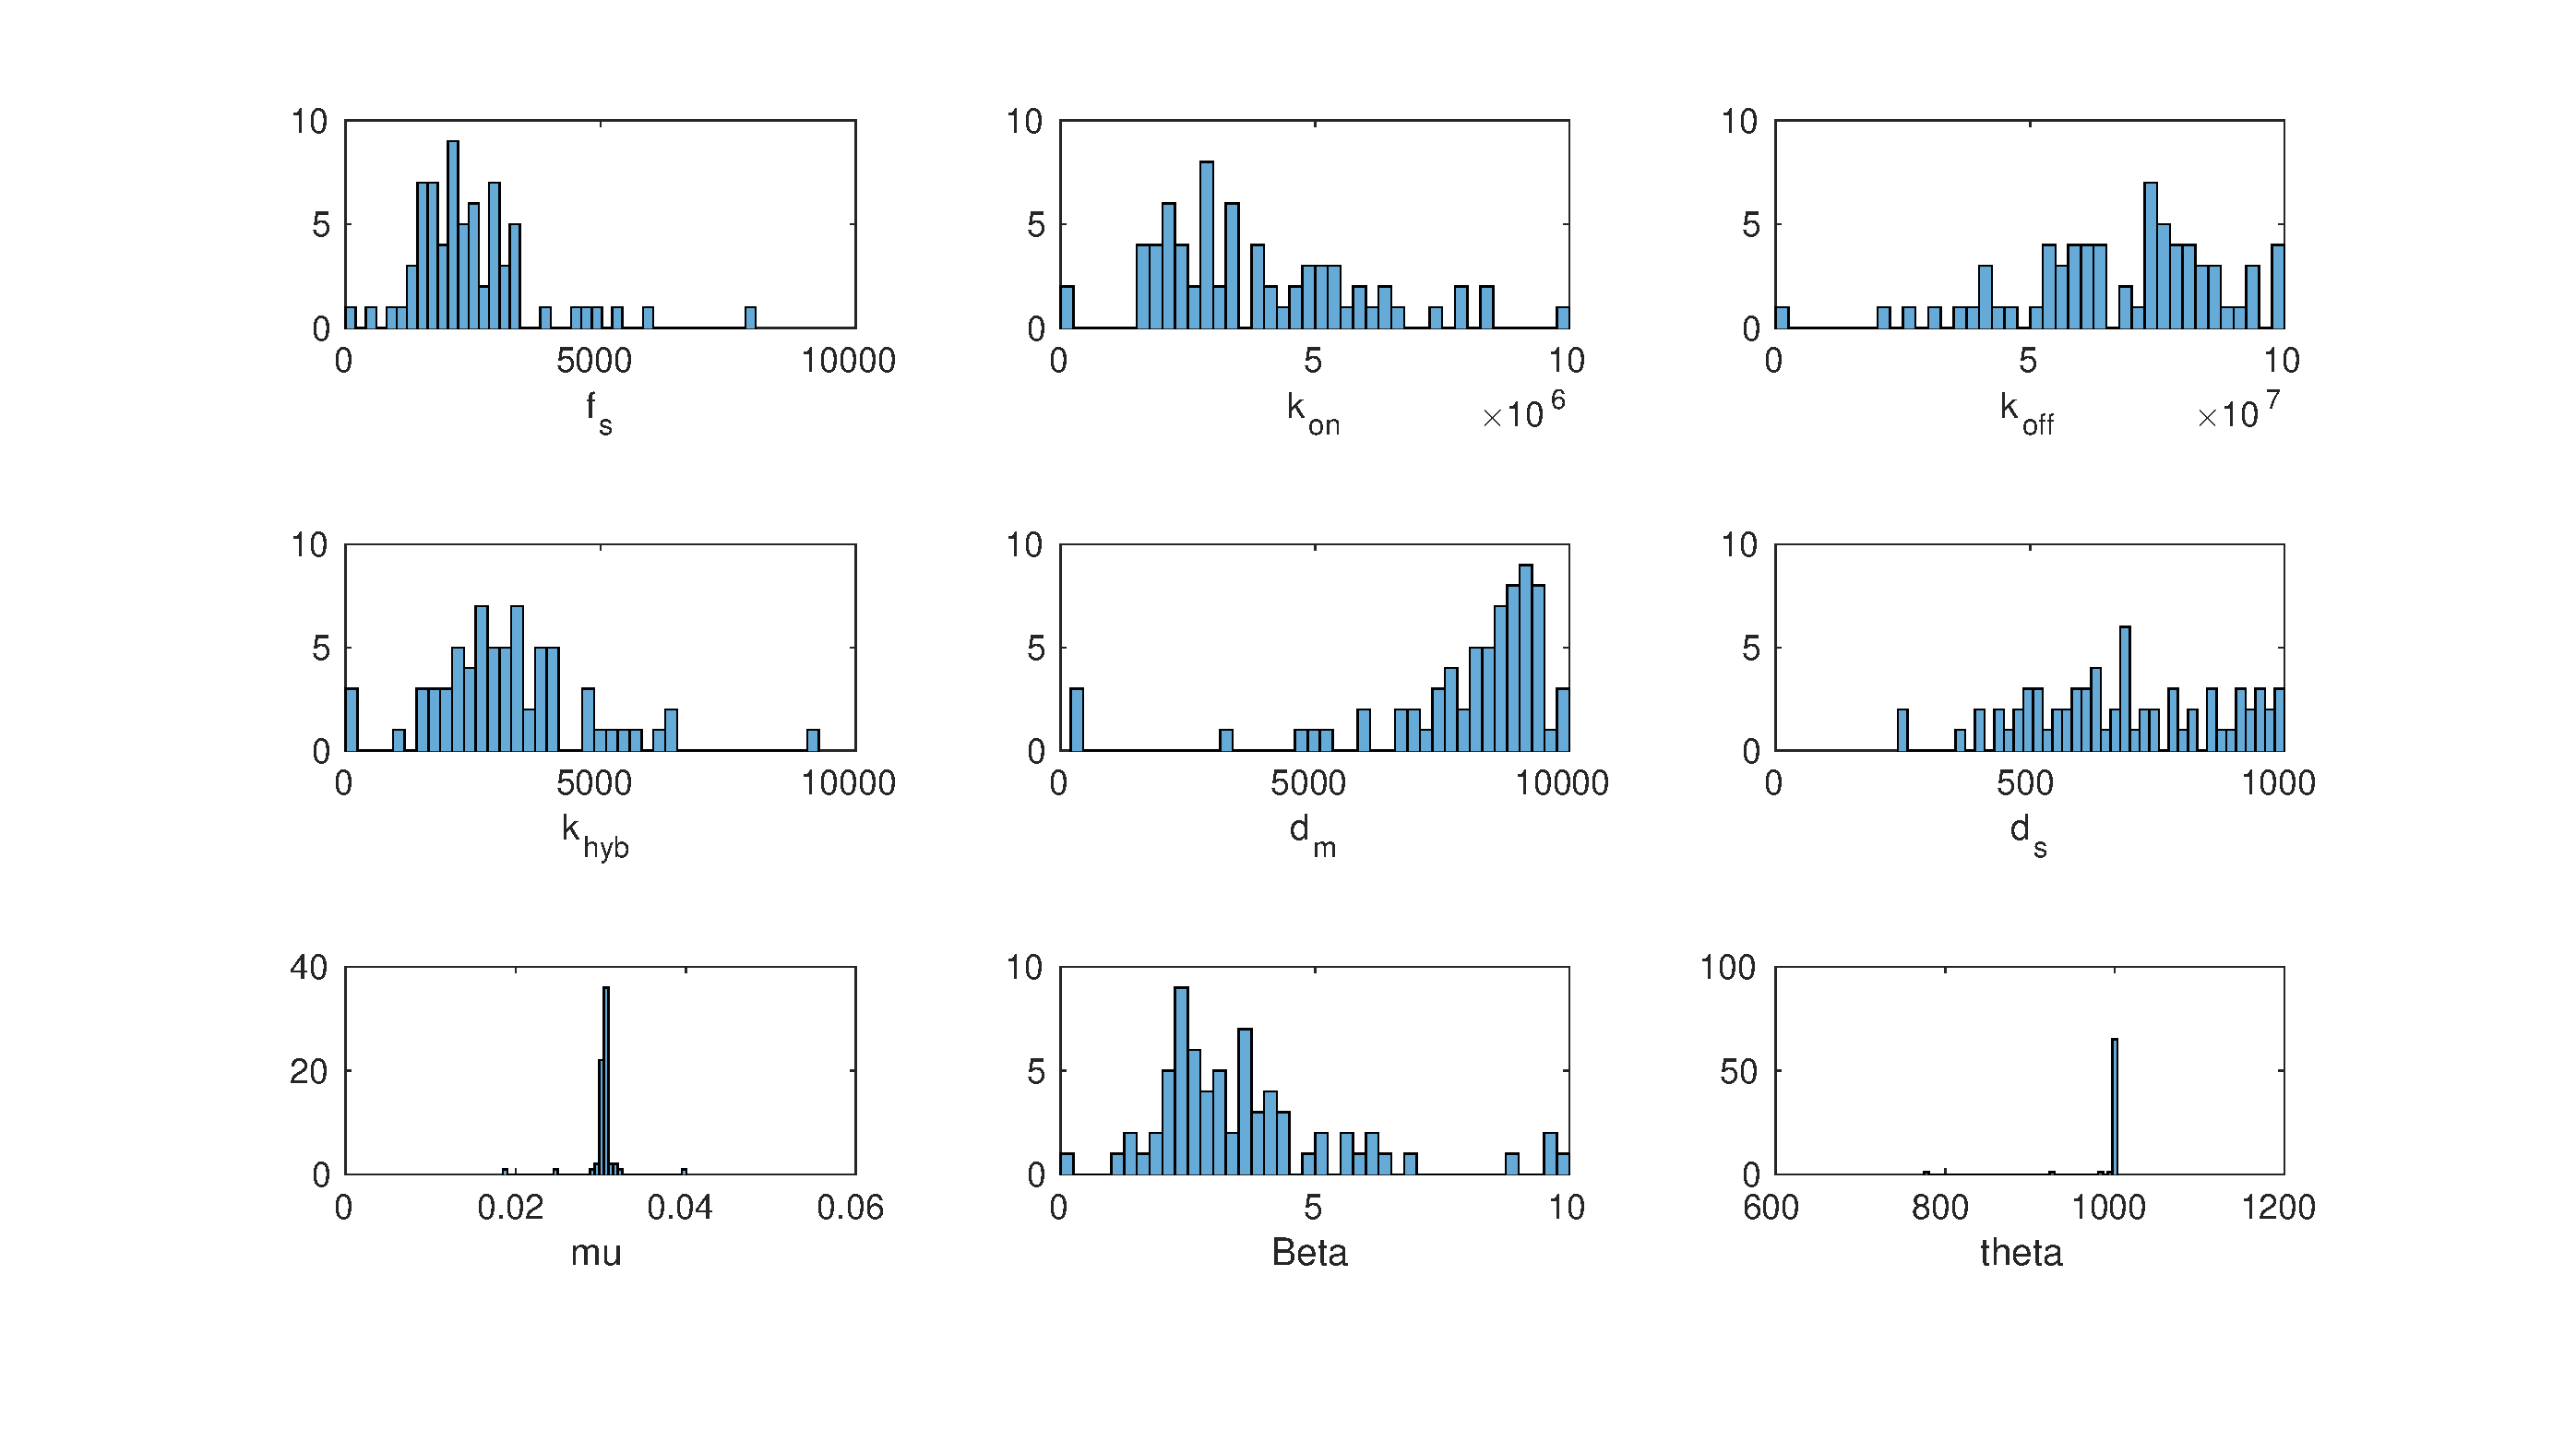
\includegraphics[scale = 0.4]{13_9_14_7_hist}
        \caption{Histogram of estimated parameter values, found from 100 runs of the CMA-ES algorithm. Fitted to both the  \textit{13\_9} and \textit{14\_7} datasets.}
        \label{}
\end{figure}

\begin{figure}[H]
   \centering
        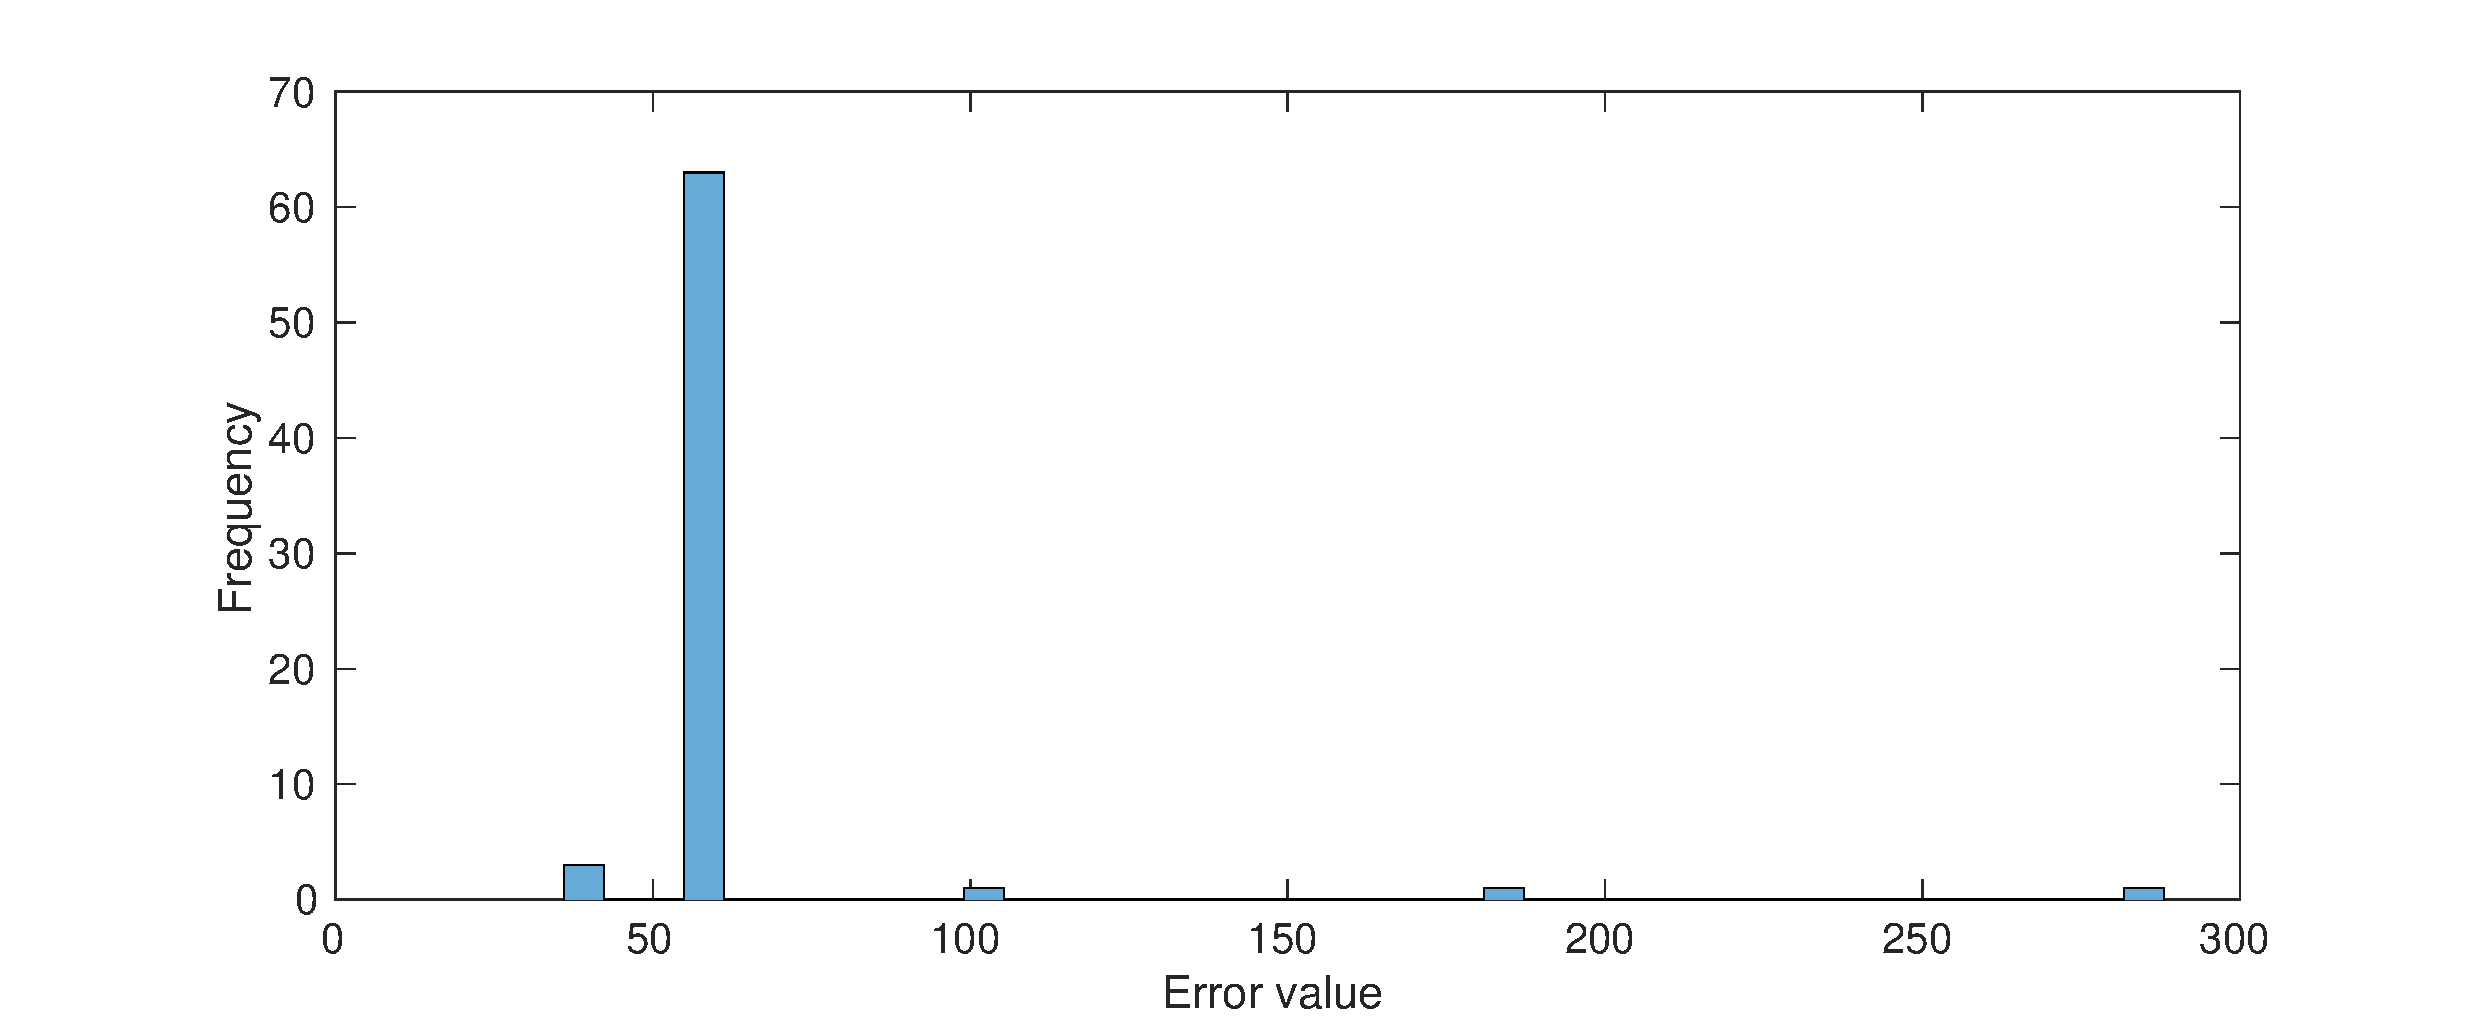
\includegraphics[scale = 0.3]{13_9_14_7_f_hist}
        \caption{Error values found from 100 initial parameter estimates. Fitted to both the  \textit{13\_9} and \textit{14\_7} datasets.}
        \label{}
\end{figure}

\end{document}



\section{Model Fixed Point}
\label{ModelFixedPoint}
\setcounter{figure}{0}   


\begin{figure*}[!t]
% ensure that we have normalsize text
\tiny
% Store the current equation number.
\setcounter{MYtempeqncnt}{\value{equation}}
% Set the equation number to one less than the one
% desired for the first equation here.
% The value here will have to changed if equations
% are added or removed prior to the place these
% equations are referenced in the main text.
\setcounter{equation}{5}
\begin{equation}
\label{eqn_dbl_x}
y\to \frac{\sqrt{2 (\text{am}+\text{as}) k_{\text{on}} \left(\mu +\delta _m\right) \left(\mu +\delta _s\right) \left(k_{\text{hyb}}+\delta _m\right)
   \left(k_{\text{hyb}}+k_{\text{off}}+\delta _m\right)+(\text{am}-\text{as})^2 k_{\text{on}}^2 \left(k_{\text{hyb}}+\delta _m\right){}^2+\left(\mu +\delta _m\right){}^2
   \left(\mu +\delta _s\right){}^2 \left(k_{\text{hyb}}+k_{\text{off}}+\delta _m\right){}^2}+(\text{am}+\text{as}) k_{\text{on}} \left(k_{\text{hyb}}+\delta
   _m\right)+\left(\mu +\delta _m\right) \left(\mu +\delta _s\right) \left(k_{\text{hyb}}+k_{\text{off}}+\delta _m\right)}{2 k_{\text{on}} \left(k_{\text{hyb}}+\delta
   _m\right){}^2}
\end{equation}
\begin{equation}
\label{eqn_dbl_y}
m\to -\frac{\sqrt{2 (\text{am}+\text{as}) k_{\text{on}} \left(\mu +\delta _m\right) \left(\mu +\delta _s\right) \left(k_{\text{hyb}}+\delta _m\right)
   \left(k_{\text{hyb}}+k_{\text{off}}+\delta _m\right)+(\text{am}-\text{as})^2 k_{\text{on}}^2 \left(k_{\text{hyb}}+\delta _m\right){}^2+\left(\mu +\delta _m\right){}^2
   \left(\mu +\delta _s\right){}^2 \left(k_{\text{hyb}}+k_{\text{off}}+\delta _m\right){}^2}-(\text{am}-\text{as}) k_{\text{on}} \left(k_{\text{hyb}}+\delta
   _m\right)+\left(\mu +\delta _m\right) \left(\mu +\delta _s\right) \left(k_{\text{hyb}}+k_{\text{off}}+\delta _m\right)}{2 k_{\text{on}} \left(\mu +\delta _m\right)
   \left(k_{\text{hyb}}+\delta _m\right)}
\end{equation}
\begin{equation}
\label{eqn_dbl_y}
s\to -\frac{\sqrt{2 (\text{am}+\text{as}) k_{\text{on}} \left(\mu +\delta _m\right) \left(\mu +\delta _s\right) \left(k_{\text{hyb}}+\delta _m\right)
   \left(k_{\text{hyb}}+k_{\text{off}}+\delta _m\right)+(\text{am}-\text{as})^2 k_{\text{on}}^2 \left(k_{\text{hyb}}+\delta _m\right){}^2+\left(\mu +\delta _m\right){}^2
   \left(\mu +\delta _s\right){}^2 \left(k_{\text{hyb}}+k_{\text{off}}+\delta _m\right){}^2}+(\text{am}-\text{as}) k_{\text{on}} \left(k_{\text{hyb}}+\delta
   _m\right)+\left(\mu +\delta _m\right) \left(\mu +\delta _s\right) \left(k_{\text{hyb}}+k_{\text{off}}+\delta _m\right)}{2 k_{\text{on}} \left(\mu +\delta _s\right)
   \left(k_{\text{hyb}}+\delta _m\right)}
\end{equation}
\begin{equation}
\frac{k_{\text{hyb}} \left(\sqrt{2 (\text{am}+\text{as}) k_{\text{on}} \left(\mu +\delta _m\right) \left(\mu +\delta _s\right) \left(k_{\text{hyb}}+\delta _m\right)
   \left(k_{\text{hyb}}+k_{\text{off}}+\delta _m\right)+(\text{am}-\text{as})^2 k_{\text{on}}^2 \left(k_{\text{hyb}}+\delta _m\right){}^2+\left(\mu +\delta _m\right){}^2
   \left(\mu +\delta _s\right){}^2 \left(k_{\text{hyb}}+k_{\text{off}}+\delta _m\right){}^2}+(\text{am}+\text{as}) k_{\text{on}} \left(k_{\text{hyb}}+\delta
   _m\right)+\left(\mu +\delta _m\right) \left(\mu +\delta _s\right) \left(k_{\text{hyb}}+k_{\text{off}}+\delta _m\right)\right)}{2 k_{\text{on}} \left(\mu +\delta
   _m\right) \left(k_{\text{hyb}}+\delta _m\right){}^2}
\end{equation}
% Restore the current equation number.
\setcounter{equation}{\value{MYtempeqncnt}}
% IEEE uses as a separator
\hrulefill
% The spacer can be tweaked to stop underfull vboxes.
\vspace*{4pt}
\end{figure*}